% template from https://fachschaft.tf.uni-freiburg.de/informationen/dokumentvorlagen
%
%
%
% documentclass options:
\documentclass[11pt,
  a4paper,
  parskip=half, % This is some extra vertical space between paragraphs, the suggestion is 2cm which is really ugly, so we use what koma script gives us
  % you can also set it to full for even more space. But there is a bad tex style decision: parskip also changes the spacing between listitems such as
  % enumerate and itemize. For this purpose we include the enumitem package and set itemsep=.5em, of course you can change this
  BCOR=10mm, % BCOR is binding correction
  ngerman,
  % if you'd rather have a one sided thesis, add `oneside' to the documentclass
  % onside,
  % ngerman is needed for hyphenation if the thesis contains parts written in German, switch order with english if you write mainly in English.
  % Remember to change order in the babel package (below) as well.
  % Last language is the preferred one.
  english]{scrbook}
\usepackage[ngerman,english]{babel} % If you write mainly in English change order to ngerman, english. Also change that in the documentclass options above.
% Include of titling must happen before \title etc.
% that's why it's not in setup.tex
\usepackage{titling}
\title{Semantic approaches to citation recommendation}
\author{Tarek Saier}

% Change to your first examiner
% The ~ enables non sentence spacing after a period
\newcommand{\firstexaminer}{Prof.~Dr.~Georg Lausen}
% Change to your second examiner, some undergraduate studies don't have a second examiner
% in this case just comment out the following line
\newcommand{\secondexaminer}{Prof.~Dr.~Christian Schindelhauer}
% Change to your adivers
\newcommand{\advisers}{Dr.~Michael F{\"{a}}rber}

% include all packages and define commands in setup.tex

%------------------------------------------------------------------------------
%       package includes
%------------------------------------------------------------------------------
    % font encoding is set up for pdflatex, for other environments see
    % http://tex.stackexchange.com/questions/44694/fontenc-vs-inputenc
    \usepackage[T1]{fontenc}  % 8-bit fonts, improves handling of hyphenations
    \usepackage[utf8]{inputenc}  % remove if engine is switched to xelatex
    % provides `old' commands for table of contents. Eases the ability to switch
    % between book and scrbook
    \usepackage{scrhack}

    % better looking fonts
    \usepackage[tt=false, type1=true]{libertine}
    \usepackage{libertinust1math}


    % ------------------- layout, default -------------------
    % adjust the style of float's captions, separated from text to improve readabilty
    \usepackage[labelfont=bf, labelsep=colon, format=hang, textfont=singlespacing]{caption}
    % With format = hang your caption will look like this:
    % Figure 1: Lorem ipsum dolor sit amet,
    %           consectetuer adipiscing elit.
    %           Ut purus elit, vestibulum
    % If you instead want
    % Figure 1: Lorem ipsum dolor sit amet,
    % consectetuer adipiscing elit. Ut purus
    % elit, vestibulum
    % change to format=plain
    \usepackage{chngcntr}  % continuous numbering of figures/tables over chapters
    \counterwithout{equation}{chapter}
    \counterwithout{figure}{chapter}
    \counterwithout{table}{chapter}

    % Uncomment the following line if you switch from scrbook to book
    % and comment the setkomafont line
    %\usepackage{titlesec}  % remove "Chapter" from the chapter title
    %\titleformat{\chapter}[hang]{\bfseries\huge}{\thechapter}{2pc}{\huge}
    \setkomafont{chapter}{\normalfont\bfseries\huge}

    \usepackage{setspace}  % Line spacing
    \onehalfspacing
    % \doublespacing  % uncomment for double spacing, e.g. for annotations in correction

    % ------------------- functional, default-------------------
    \usepackage[dvipsnames]{xcolor}  % more colors
    \usepackage{array}  % custom format per column in table - needed on the title page
    \usepackage{graphicx}  % include graphics
    \usepackage{subfig}  % divide figure, e.g. 1(a), 1(b)...
    \usepackage{amsmath}  % |
    \usepackage{amsthm}   % | math, bmatrix etc
    \usepackage{amsfonts} % |
    \usepackage{calc}  % calculate within LaTeX
    \usepackage[unicode=true,bookmarks=true,bookmarksnumbered=true,
                bookmarksopen=true,bookmarksopenlevel=1,breaklinks=false,
                pdfborder={0 0 0},backref=false,colorlinks=false]{hyperref}
    \usepackage{etoolbox} % if-else commands


    %==========================================
    % You might not need the following packages, I only included them as they
    % are needed for the example floats
    % ------------------- functional, custom -------------------
    \usepackage{algorithm,algpseudocode}
    \usepackage{bm}  % bold greek variables (boldmath)
    % \usepackage{tikz}
    % \usetikzlibrary{positioning}  % use: above left of, etc

    % Improves general appearance of the text
    \usepackage[protrusion=true,expansion=true, kerning]{microtype}
    % \usepackage[protrusion=true]{microtype} % in case a switch to xelatex is
    %                                           necessary
    \usepackage{enumitem}

    % usually you don't need this, just for demonstration of a longer caption
    % \usepackage{lipsum}

    % toprule/midrule style tables
    \usepackage{booktabs}
    % make footnotes in tables work
    \usepackage{footnote}
    \makesavenoteenv{tabular}
    \makesavenoteenv{table}
    % enable listings
    \usepackage{listings}
    \lstset{literate=
      {Ş}{{\c{S}}}1 {ğ}{{\v{g}}}1,
      frame=top,frame=bottom,
      breaklines=true,
      basicstyle=\linespread{1}\footnotesize\ttfamily,
      escapeinside={(*}{*)}
    }

%------------------------------------------------------------------------------
%       (re)new commands / settings
%------------------------------------------------------------------------------
    % ----------------- referencing ----------------
    \newcommand{\secref}[1]{Section~\ref{#1}}
    \newcommand{\chapref}[1]{Chapter~\ref{#1}}
    \renewcommand{\eqref}[1]{Equation~(\ref{#1})}
    \newcommand{\figref}[1]{Figure~\ref{#1}}
    \newcommand{\tabref}[1]{Table~\ref{#1}}

    % ------------------- colors -------------------
    \definecolor{darkgreen}{rgb}{0.0, 0.5, 0.0}
    % Colors of the Albert Ludwigs University as in
    % https://www.zuv.uni-freiburg.de/service/cd/cd-manual/farbwelt
    \definecolor{UniBlue}{RGB}{0, 74, 153}
    \definecolor{UniRed}{RGB}{193, 0, 42}
    \definecolor{UniGrey}{RGB}{154, 155, 156}


    % ------------------- layout -------------------
    % prevents floating objects from being placed ahead of their section
    \let\mySection\section\renewcommand{\section}{\suppressfloats[t]\mySection}
    \let\mySubSection\subsection\renewcommand{\subsection}{\suppressfloats[t]\mySubSection}


    % ------------------- marker commands -------------------
    % ToDo command
    \newcommand{\todo}[1]{\textbf{\textcolor{red}{(TODO: #1)}}}
    \newcommand{\extend}[1]{\textbf{\textcolor{darkgreen}{(EXTEND: #1)}}}
    % Lighter color to note down quick drafts
    \newcommand{\draft}[1]{\textbf{\textcolor{NavyBlue}{(DRAFT: #1)}}}


    % ------------------- math formatting commands -------------------
    % define vectors to be bold instead of using an arrow
    \renewcommand{\vec}[1]{\mathbf{#1}}
    \newcommand{\mat}[1]{\mathbf{#1}}
    % tag equation with name
    \newcommand{\eqname}[1]{\tag*{#1}}


    % ------------------- pdf settings -------------------
    % ADAPT THIS
    \hypersetup{pdftitle={\thetitle},
                pdfauthor={\theauthor},
                pdfsubject={Master's thesis at the Albert Ludwig University of Freiburg},
                pdfkeywords={citation recommendation, recommender system, data set, master thesis},
                pdfpagelayout=OneColumn, pdfnewwindow=true, pdfstartview=XYZ, plainpages=false}


    %==========================================
    % You might not need the following commands, I only included them as they
    % are needed for the example floats

    % ------------------- Tikz styles -------------------
    % \tikzset{>=latex}  % arrow style

    % ------------------- algorithm ---------------------
    % Command to align comments in algorithm
    \newcommand{\alignedComment}[1]{\Comment{\parbox[t]{.35\linewidth}{#1}}}
    % define a foreach command in algorithms
    \algnewcommand\algorithmicforeach{\textbf{foreach}}
    \algdef{S}[FOR]{ForEach}[1]{\algorithmicforeach\ #1\ \algorithmicdo}

    % line spacing should be 1.5
    \renewcommand{\baselinestretch}{1.5}

    % set distance between items in a list, for more details see the
    % enumitem package: https://www.ctan.org/pkg/enumitem
    \setlist{topsep=0pt,itemsep=0ex,partopsep=1ex,parsep=0ex}


\begin{document}
    \pagestyle{empty} % no header and no page number
    % disable hyper links to remove warning "destination with same identifier"
    % this means within this section nothing can be referenced with a hyperlink
    \hypersetup{pageanchor=false}

    % enable/disable, depending on your chosen language
    
\begin{titlepage}
\begin{center}

\newcommand{\HorizontalLine}{\rule{\linewidth}{0.3mm}}

{\Large Master's Thesis}\\[1.3cm]


% _____________________________________________________________________________
\HorizontalLine \\[0.4cm]
% Write your title in a fancy way like this if you want to customize it, otherwise simply let tex do it for you
% \begin{spacing}{3}
%     {\huge \bfseries The Long, Long } \\
%     {\huge \bfseries Long Long} \\
%     {\huge \bfseries Title}\\
% \end{spacing}
{ \huge \bfseries \thetitle }
\HorizontalLine \\[1.5cm]
% _____________________________________________________________________________


{\Huge \theauthor} \\[2cm]


\begin{tabular}[hc]{>{\huge}l >{\huge}l}
  Examiners: & \firstexaminer \\[0.3cm]
             & \secondexaminer \\[1.2cm]
\end{tabular}
\vfill  % move the following text to the bottom

\Large {
    Albert-Ludwigs-University Freiburg\\
    Faculty of Engineering\\
    Department of Computer Science\\
    Chair of Databases and Information Systems\\[1cm]

    April 30\textsuperscript{th}, 2019\\
}
\end{center}
\end{titlepage}

\thispagestyle{empty}
% title page back
\ \vfill \ \\  % at least one space required before vfill
\
\textbf{Writing Period}            \smallskip{} \\
15.\,10.\,2018 -- 30.\,04.\,2019   \bigskip{} \\
\
\textbf{First Examiner}                  \smallskip{} \\
\firstexaminer                     \bigskip{} \\
\
% If there is a second examiner include it
\ifdef{\secondexaminer}
	{
	% Include
	\textbf{Second Examiner \& Supervisor}       \smallskip{} \\
	\secondexaminer                \bigskip{} \\
	\
	}
	{
	% No second examiner, ignore
	}
% \textbf{Supervisor}                  \smallskip{} \\
% \advisers

    \begin{titlepage}
\begin{center}

\newcommand{\HorizontalLine}{\rule{\linewidth}{0.3mm}}

{\Large Master-Thesis}\\[1.3cm]


% _____________________________________________________________________________
\HorizontalLine \\[0.4cm]
% Write yourtitle in a fancy way like this if you want to customize it, otherwise simply let tex do it for you
% \begin{spacing}{3}
%     {\huge \bfseries Der Lange, Lange } \\
%     {\huge \bfseries Lange Lange} \\
%     {\huge \bfseries Titel}\\
% \end{spacing}
{ \huge \bfseries \thetitle }
\HorizontalLine \\[1.5cm]
% _____________________________________________________________________________


{\Huge \theauthor} \\[2cm]


\begin{tabular}[hc]{>{\huge}l >{\huge}l}
  Gutachter: & \firstexaminer \\[0.3cm]
             & \secondexaminer \\[1.2cm]
\end{tabular}
\vfill  % move the following text to the bottom

\Large {
    Albert-Ludwigs-Universität Freiburg\\
    Technische Fakultät\\
    Institut für Informatik\\
    Lehrstuhl für Datenbanken und Informationssysteme\\[1cm]

    30. April 2019
    \\
}
\end{center}
\end{titlepage}

\thispagestyle{empty}
% title page back
\ \vfill \ \\  % at least one space required before vfill
\
\textbf{Bearbeitungszeit}            \smallskip{} \\
15.\,10.\,2018 -- 30.\,04.\,2019   \bigskip{} \\
\
\textbf{Erstgutachter}                  \smallskip{} \\
\firstexaminer                      \bigskip{} \\
\
% If there is a second examiner include it
\ifdef{\secondexaminer}
	{
	% Include
	\textbf{Zweitgutachter \& Betreuer}        \smallskip{} \\
	\secondexaminer                \bigskip{} \\
	\
	}
	{
	% No second examiner, ignore
	}
% \textbf{Betreuer}                  \smallskip{} \\
% \advisers


    \pagestyle{plain} % remove chapter name from top, page number at the bottom
    % use \pagestyle{headings} for having the chapter on top of the pages
    % if you want a more fancy header use \usepackage[automark,headsepline]{scrlayer-scrpage}
    % and read about it in the KOMA script documentation, https://www.ctan.org/pkg/koma-script
    \frontmatter  % roman page numbers
    % official declaration from the examination office
% copied from https://www.tf.uni-freiburg.de/de/studium-lehre/a-bis-z-studium/dokumente/Declarationforthefinalthesis.pdf

\chapter*{Declaration}

I hereby declare, that I am the sole author and composer of my thesis and that no other sources or learning aids, other than those listed, have been used. Furthermore, I declare that I have acknowledged the work of others by providing detailed references of said work.  \newline
I also hereby declare, that my thesis has not been prepared for another examination
or assignment, either in its entirety or excerpts thereof.
\\[3\normalbaselineskip]
\begin{tabular}{p{\textwidth/2} l}
  \rule{\textwidth/3}{0.4pt}   &   \rule{\textwidth/3}{0.4pt} \\
  Place, Date                  &   Signature
\end{tabular}

    \chapter*{Abstract}
New research is being published at a rate, at which it is %
%practically
infeasible for many scholars, to read and assess everything possibly %
%/that could possibly be
relevant to their work. %
In pursuit of a remedy, efforts towards automated processing of publications, like semantic modelling of papers to facilitate their digital handling, and the development of information filtering systems, are an active area of research. %
% maybe add a sentence here, leading from research in this
% area *in general* to citation recommendation
In this thesis, we investigate the semantic modelling of citation contexts for the purpose of citation recommendation. For this, we generate a large data set with accurate citation information from publications' \LaTeX{} sources on arXiv.org. Using this data set, we develop recommendation models based on entities and claim structures. To assess the effectiveness and conceptual soundness of our models, we perform a large offline evaluation on our own as well as several established data sets and furthermore conduct a user study. Our findings show that the models can outperform a non-semantic baseline model and do, indeed, capture the kind of information they're conceptualized for.
%In evaluating our models on several data sets and through a user study, we show that they can outperform a non-semantic baseline and are especially well suited for the recommendation of the types of citations they're conceptualized for.

%Citation recommendation systems, a possible remedy, 
%Researchers spent a considerable amount of time identifying publications that are worthwhile reading and appropriate to reference. The development of systems to aid in these tasks is an active area of research.
%Citations are the means by which scholars relate their research to existing work, 

\chapter*{Zusammenfassung}
fu bar

    \tableofcontents
    \listoffigures
    \listoftables
    \listofalgorithms
    \hypersetup{pageanchor=true}  % re-enable hyperlinking

    \mainmatter  % Arabic page numbers
    \chapter{Introduction}\label{chap:introduction}
\section{Motivation}
Citations are a central building block of scholarly discourse. They are the means by which scholars relate their research to existing work---be it in backing up claims, criticising, naming examples or engaging in any other form. Citing in a meaningful way requires an author to be aware of publications relevant to their work.
Here, the ever increasing amount of new reseach publications per year poses a serious challenge. Even with academic search engines like Goolge Scholar and CiteSeer$^X$ at our disposal, identifying publications that are worthwhile to examine and appropriate to reference remains a time consuming task.

It is therefore not suprising that methods to aid researchers in these tasks have been and still are being actively researched. While diverse in nature, the common core of these efforts is the goal to utilize the automated processing of publications. This can be achieved by either extracting information from publications as they are~\cite{Nasar2018,Beel2016}, or by introducing explicit semantic representations of their content or interrelations to facilitate automated processing~\cite{BuckinghamShum2000,Schneider2013,Jaradeh2019}. % TODO: mby distinguish between metadata and annotation/representation of content here (for the latter mby name JATS)
Once processed, a typical method is to harvest human made citations, analyze them~\cite{Abujbara2013,Teufel2006a} and use them for example to recommend papers~\cite{Beel2016} or aid in document exploration~\cite{Berger2016}. Although systems like this have existed for over 20 years~\cite{Bollacker1998,Beel2016}, there is not a lot of work looking into the use of explicit semantic representations for the recommendation of papers.
% ,Kitamoto2015 (after BuckinghamShum and Schneider)
% TODO: mby add sth about what the prospective benefits of semantic representations would be (e.g. if rather advanced model: search for citations for certain claims instead of just keyword based)
This is why this thesis will investiage their application. More specifically, we will concentrate on the task of recommending papers for citation---as opposed to, for example, discovery. What this encompasses will be described in more detail in the following section.

%Teufel2006b

% Systems for recommending papers have existed since 1998~\cite{Bollacker1998,Beel2016}. The closely related field of citation analysis has an even longer history that spans multiple disciplices including applied linguistics, history and sociology of sience and information science~\cite{Swales1986,White2004}.

% also there’s different approaches to it (collab.fil. / content based fil.(input=paper / input=sentence / input=sentence+one citation\cite{Kobayashi2018} / input=abstract\cite{Ayala-Gomez2018}) / graph based)

\section{Problem setting}\label{sec:problemsetting}
In the boradest sense, recommending papers for citation means given an input text, suggest publications that can be referred to from within that text. In scale this can vary from specific recommendations for a section of a sentence (\emph{local} or \emph{context-based}), to general recommendations for a whole input document (\emph{global}). The task can also include deciding whether or not the input contains parts that would justify inserting a citation in the first place~\cite{He2011}. In this thesis, we will focus on local citation recommendation with the assumption that the input always allows for/requires a citation to be put in.

Another distinction to be made is between personalized and general citation recommendation. Some approaches make use of user specific information such as an author's prior citations. Collaborative filtering approaches by nature include a user model and therfore fall into this category. While personalization can improve recommendation, it limits the approach to users that are willing to share personal information. % also if prior own publications would be needed (to see what authors, venues, fields of study one cites) there would be an interesting version of the could start problem. worth mentioning?
We therefore limit ourselves to purely content based filtering approaches.
% TODO: add argument for only using contexts to describe cited docs and not also title, abstract, metadata (mby cite \cite{Elkiss2008}) (possible argument: first only investigate semantic representations of citation contexts, then (future work) look into combining this information with other data)

A last clarification has to be made concerning the term \emph{explicit semantic representations}. This is to be understood as a differentiation from the mere use of unstructured text. A most prominent example for explicit semantic representations would be the structure of the Semantic Web~\cite{Berners-Lee2001}. In the context of citation recommendation as briefly outlined above this means representing citations in a semantically meaningful way as opposed to just relying on syntactical information like n-grams or bag-of-words representations.

The problem setting can be summarized as follows. To investigate is, the applicability of and requirements for the use of explicit semantic representations for content based, local citation recommendation. The following section will outline how this investigation is performed.

\section{Method}\label{sec:method}
In order to assess if and how explicit semantic representations can benefit citation recommendation we investigate the use of named entities as well as claim structures. For the evaluation of our models in a realistic setting we generate a large data set that allows for the extraction of precise citation marker positions. To ensure comparability with other approaches we also perform evaluations on existing data sets as far as possible.

Extend to mention offline and online eval

Extend moar

\section{Contributions}\label{sec:contributions}
The data set

Entity and claim based models

Insights into open problems with building claim models around citations (b/c of non-integral citation styles)

\section{Document structure}\label{sec:documentstructure}
foo bar

Copypasta of useful stuff below.
\begin{itemize}
    \item Put a tilde (nbsp) in front of citations~\cite{Moravcsik1975}.
    \item \todo{Do this!}
    \item \extend{Write more when new results are out!}
    \item \draft{Hacky text!}
    \item \chapref{chap:introduction} % also \chapref{} \secref{sec:XY} \eqref{} \figref{} \tabref{}
    \item the colors of the Uni
    \begin{itemize}
        \item {\color{UniBlue}UniBlue}
        \item {\color{UniRed}UniRed}
        \item {\color{UniGrey}UniGrey}
    \end{itemize}
    \item a command for naming matrices $\mat{G}$, and naming vectors $\vec{a}$. This overwrites the default behavior of having an arrow over vectors, sticking to the naming conventions  normal font for scalars, bold-lowercase for vectors, and bold-uppercase for matrices.
    \item named equations:
        \begin{align}
            d(a,b) &= d(b,a)\\ \eqname{symmetry}
        \end{align}
    \item Use ``these'' for citing, not "these"
    \item If an equation is at the end of a sentence, add a full stop. If it's not the end, add a comma: {$a= b + c$~~~~(1),}
    \item \url{https://en.wikipedia.org}
    \item Do not overuse footnotes\footnote{\url{https://en.wikipedia.org}} if possible.
\end{itemize}

    \chapter{Related Work}\label{chap:relatedwork}
lots. pick wisely.

Leveraging Semantic Annotations to Link Wikipedia and News Archives\cite{Mishra2016}

Using NEL + dependency trees for music recommendation\cite{Sordo2015}

use citeulike tags as "academic concepts" for paper recommendation\cite{Jiang2012}

Capturing knowledge of user preferences: ontologies in recommender systems\cite{Middleton2001,Middleton2004}

continue in Beel2016 on p. 318 (right side)

    \chapter{Background}\label{chap:background}
In this chapter we will define important terms and lay out the theoretical background for the remainder of the thesis.

\section{Definition of terms}
\paragraph{Citation} The term \emph{``citation''} can refer to both the act of citing as well as the occurrence of being cited. This can be illustrated with the phrase \emph{``an author's citations''}. In \cite{Beel2016} Beel et al. write \emph{``McNee et al. assumed that an author's citations indicate a positive vote for a paper [93].''} (the author cites), while Myers~\cite{Myers1970} writes \emph{``Thus, the number of an author's citations, in this study, means the number of articles in which one or more of his publications were cited.''} (the author is being cited). Like the latter example we will make an effort to use the term unambiguously.
% also: \cite{Beel2016} \emph{``a few articles gained many citations (the maximum was 528 citations for [43]) and many articles had few citations, see Fig. 3.''} -> passive
\paragraph{Citation marker} A citation marker is a string of text that identifies an entry within a document's reference section. Examples are ``[27]'', ``[Bol98]'' and ``(He, 2010)''. These are placed within the document whenever the author refers to one of the documents in the reference section.
\paragraph{Citation context} The context of a citation is the text surrounding its citation marker. Typical sizes are 1--3 sentences. The sentence containing the marker is also sometimes referred to as ``citing sentence''. 

\begin{table}
\centering
    \caption[Examples of citations and their categorization into integral/non-integral as well as syntactic/non-syntactic.]{Examples of citations and their categorization into integral/non-integral (values left of split) as well as syntactic/non-syntactic (values right of split).}
    \label{tab:integralsyntactic}
\begin{center}
    \begin{tabular}{llllll|ll}%m{8cm}
    \toprule
    Context excerpt (citation marker {\color{UniBlue}highlighted}) & \rotatebox{90}{Swales~\cite{Swales1990}} & \rotatebox{90}{Hyland~\cite{Hyland1999}} & \rotatebox{90}{Thompson~\cite{Thompson2001}} & \rotatebox{90}{Okamura~\cite{Okamura2008}} & \rotatebox{90}{Lamers et al.~\cite{Lamers2018}} & \rotatebox{90}{Whidby et al.~\cite{Whidby2011}} & \rotatebox{90}{Abujbara et al.~\cite{Abujbara2012}} \\
    \midrule
    ``Swales {\color{UniBlue}(1990)} has argued that ...''                 & i & i & i & i & i & n & ? \\
    ``{\color{UniBlue}Swales (1990)} has argued that ...''                 & i & i & i & i & n & s & s \\
    ``Swales {\color{UniBlue}[42]} has argued that ...''                   & i & i & i & i & i & n & n \\
    ``Swales has argued that ... {\color{UniBlue}[42]}''                   & i & i & i & i & i & n & n \\
    ``It has been argued {\color{UniBlue}(Swales, 1990)} that ...''         & n & n & n & n & n & n & n \\
    ``It has been argued {\color{UniBlue}[42]} that ...''                  & n & n & n & n & n & n & n \\
    ``According to {\color{UniBlue}(Swales, 1990)} it is ...'' & ? & ? & ? & ? & n & s & s \\
    ``According to {\color{UniBlue}[42]} it is ...''          & n & n & n & n & n & s & s \\
    ``... has been shown (see {\color{UniBlue}(Swales, 1990)}).''           & n & n & n & n & n & s & n \\
    \bottomrule
    \end{tabular}
\end{center}
\end{table}

\paragraph{Integral and syntactic citations} There are two somewhat similar, and at first glance easily confused notions considering a citation's role within its context. They are referred to as ``integral''---in the adjectival sense close in meaning to ``essential'' or ``inherent'', not what we denote in calculus with $\int$---and ``syntactic''. Integral citations were first defined by Swales~\cite{Swales1990} in 1990 and are a frequently used~\cite{Hyland1999,Thompson2001,Okamura2008,Lamers2018} measure in discourse analysis. An integral citation is, in Swales' own words, \emph{``one in which the name of the researcher occurs in the actual citing sentence as some sentence-element''}. Thompson~\cite{Thompson2001} rephrases the definition as \emph{``citations that [...] play an explicit grammatical role within a sentence''}. While what Thompson refers to as ``citations'' might be confused with the notion of citation markers, the examples given in \cite{Thompson2001} clearly indicate that a ``citation'' is to mean an author's name in their definition. The second notion, ``syntactic'' (as used in \cite{Whidby2011} and \cite{Abujbara2012}), is concerned with whether or not a \emph{citation marker} has a grammatical role within its context. In other words, if removing the citation marker would make the citing sentence ungrammatical, then it is syntactic. Table~\ref{tab:integralsyntactic} gives an overview of examples for both concepts. Note that Lamers et al.~\cite{Lamers2018} provide a classification algorithm for integral and non-integral citations that slightly differs from Swales' original definition depending on the interpretation of a citation marker's scope, but also gives a clear classification in an edge case where Swales's definition is unclear. Furthermore note that the two ways for distinguishing syntactic and non-syntactic citations found in literature are not identical. This is in part because the method given in \cite{Abujbara2012} is kept rather simple. For the intents and purposes of this work we can follow the definitions of Lamers et al. and Whidby et al. for ``integral'' and ``syntactic'' respectively.
\paragraph{Reference} References are the entries in a document's reference section. Each reference should unambiguously identify another document that it points to. In the context of parsing reference sections we will, at times, refer to references as ``reference strings''. An example of a reference is \emph{``W. Huang, P. Mitra, and C. L. Giles, `RefSeer: A citation recommendation system,' in IEEE/ACM Joint Conference on Digital Libraries, pp. 371–374, Sep. 2014.''}.
\paragraph{Reference resolution} The act of parsing a reference string and matching it to a document identifier is what we refer to as ``reference resolution''. Examples can be found in Section~\ref{sec:refresol}.
% \paragraph{Citation recommendation} global/local  % already explained in first chapter
\paragraph{Named Entity} In natural language processing the term ``Named Entity'' (NE) describes unambiguous abstract or physical entities which have a proper name. Examples are people (Tim Berners-Lee), places (the city Taipei), organizations (the Free Software Foundation) and concepts (Okapi BM25). For a more detailed discussion of the term see~\cite{Nadeau2007}.
\paragraph{Noun phrase} A noun phrase is a group of words (or a single word) functioning grammatically as one unit, that has a noun at its head. Examples are ``\emph{example}'', ``noun \emph{phrase}'' and ``context-based co-citation \emph{recommendation}'' (head of the phrase \emph{highlighted}).
\paragraph{Claim} For the scope of this thesis we define a ``claim'' as an ideally verifiable and at least debatable statement in writing. The motivation for this definition is to capture those parts of publications, that are backed by citations. Examples are ``The boolean satisfiability problem (SAT) is NP-complete.'', ``CiteSeer was introduced in 1998.'' and ``Parsing \LaTeX{} sources is a non trivial task.''---the latter statement showcasing a not necessarily verifiable but at least debatable statement.
\paragraph{Citation recommendation} We define ``citation recommendation'' as the task of recommending publications for purpose of referencing them. The input for a recommendation is at least a citation context (optionally more, like information on the author) and the output a list of publications that can or should be referred to from within the context. To give an example, a good recommendation for the input ``CiteSeer was introduced in 1998.'' would be ``K. D. Bollacker, S. Lawrence, and C. L. Giles, \emph{`CiteSeer: An Autonomous Web Agent for Automatic Retrieval and Identification of Interesting Publications'}, AGENTS `98''.

\section{Theoretical background}
\subsection{Recommending scientific publications}
Recommending scientific publications can be approached as a variety of tasks, such as link prediction, machine translation (see Section~\ref{sec:localrelated}) and, of course, recommendation. In the following, we will take the latter perspective. Generally speaking, recommender systems are tools of discovery. In situations where a user can not reasonably be assumed to consider all available options, a recommender system's task is to identify those items that maximize a user's satisfaction, service provider's revenue or similar goal. This is typically done by calculating a score for each available item, ranking them by score and finally presenting the top ones to the user. Common domains of recommendation are shopping products and media (movies, news articles, etc.). A coarse distinction of techniques for recommendation---ignoring hybrid and less conventional cases---can be made between \emph{content-based} and \emph{collaborative filtering}. The latter exploits the similarity of user profiles for recommendation, while the former operates on the similarity of the items.~\cite{Ricci2015}

Scientific publications as a recommender domain has some atypical characteristics. One of these is the ratio of users to items. Comparing, for example, to movie recommendation, the average number of new movies listed on the Internet Movie Database (IMDb) for the last 10 years (2009--2018) is about the same as the average number of new publications in the field of high energy physics on arXiv.org for the same time span---about 9,500 new items per year in both cases. Needless to say, there is more people watching movies than doing research in high energy physics. This can mean fewer users to compare to, when using collaborative filtering methods to recommend scientific publications. Another peculiarity in this domain is the interconnectedness of items. While movies may have aspects like actors, directors, locations, etc. in common, scholarly writings not only share authors, venues, journals, etc. but are furthermore interconnected through citations. A consequence of this is the feasibility to utilize citation networks and citation contexts for recommendation.

Recommendation of scientific publications can be done for several purposes, like introducing researchers to papers they might want to read, identifying works that are relevant to a draft of a new paper or suggesting publications that can be cited in a given context. While in all of these cases the nature of the items remains the same, input and constraints for the recommendation process differ. For the discovery of papers a researcher might find worthwhile reading, the focus lies on the researcher's interest and there are no externally imposed hard constraints. In contrast, when recommending publications for the use of citation, the context of the citation plays a considerably larger role than an author's interest. There might be some leeway for personal citation style, but by and large the adequacy of a citation is dictated by its target context and the contents of candidate items. In this way, the task of citation recommendation can also be seen as a more general information retrieval problem where the citation context is the query for which adequate citations have to be identified.

Having established the relative position of the field of citation recommendation with respect to related fields, we will lay out the core concepts relevant to our approach, \emph{content based local citation recommendation by use of citation contexts}, below.

\begin{figure}
  \centering
    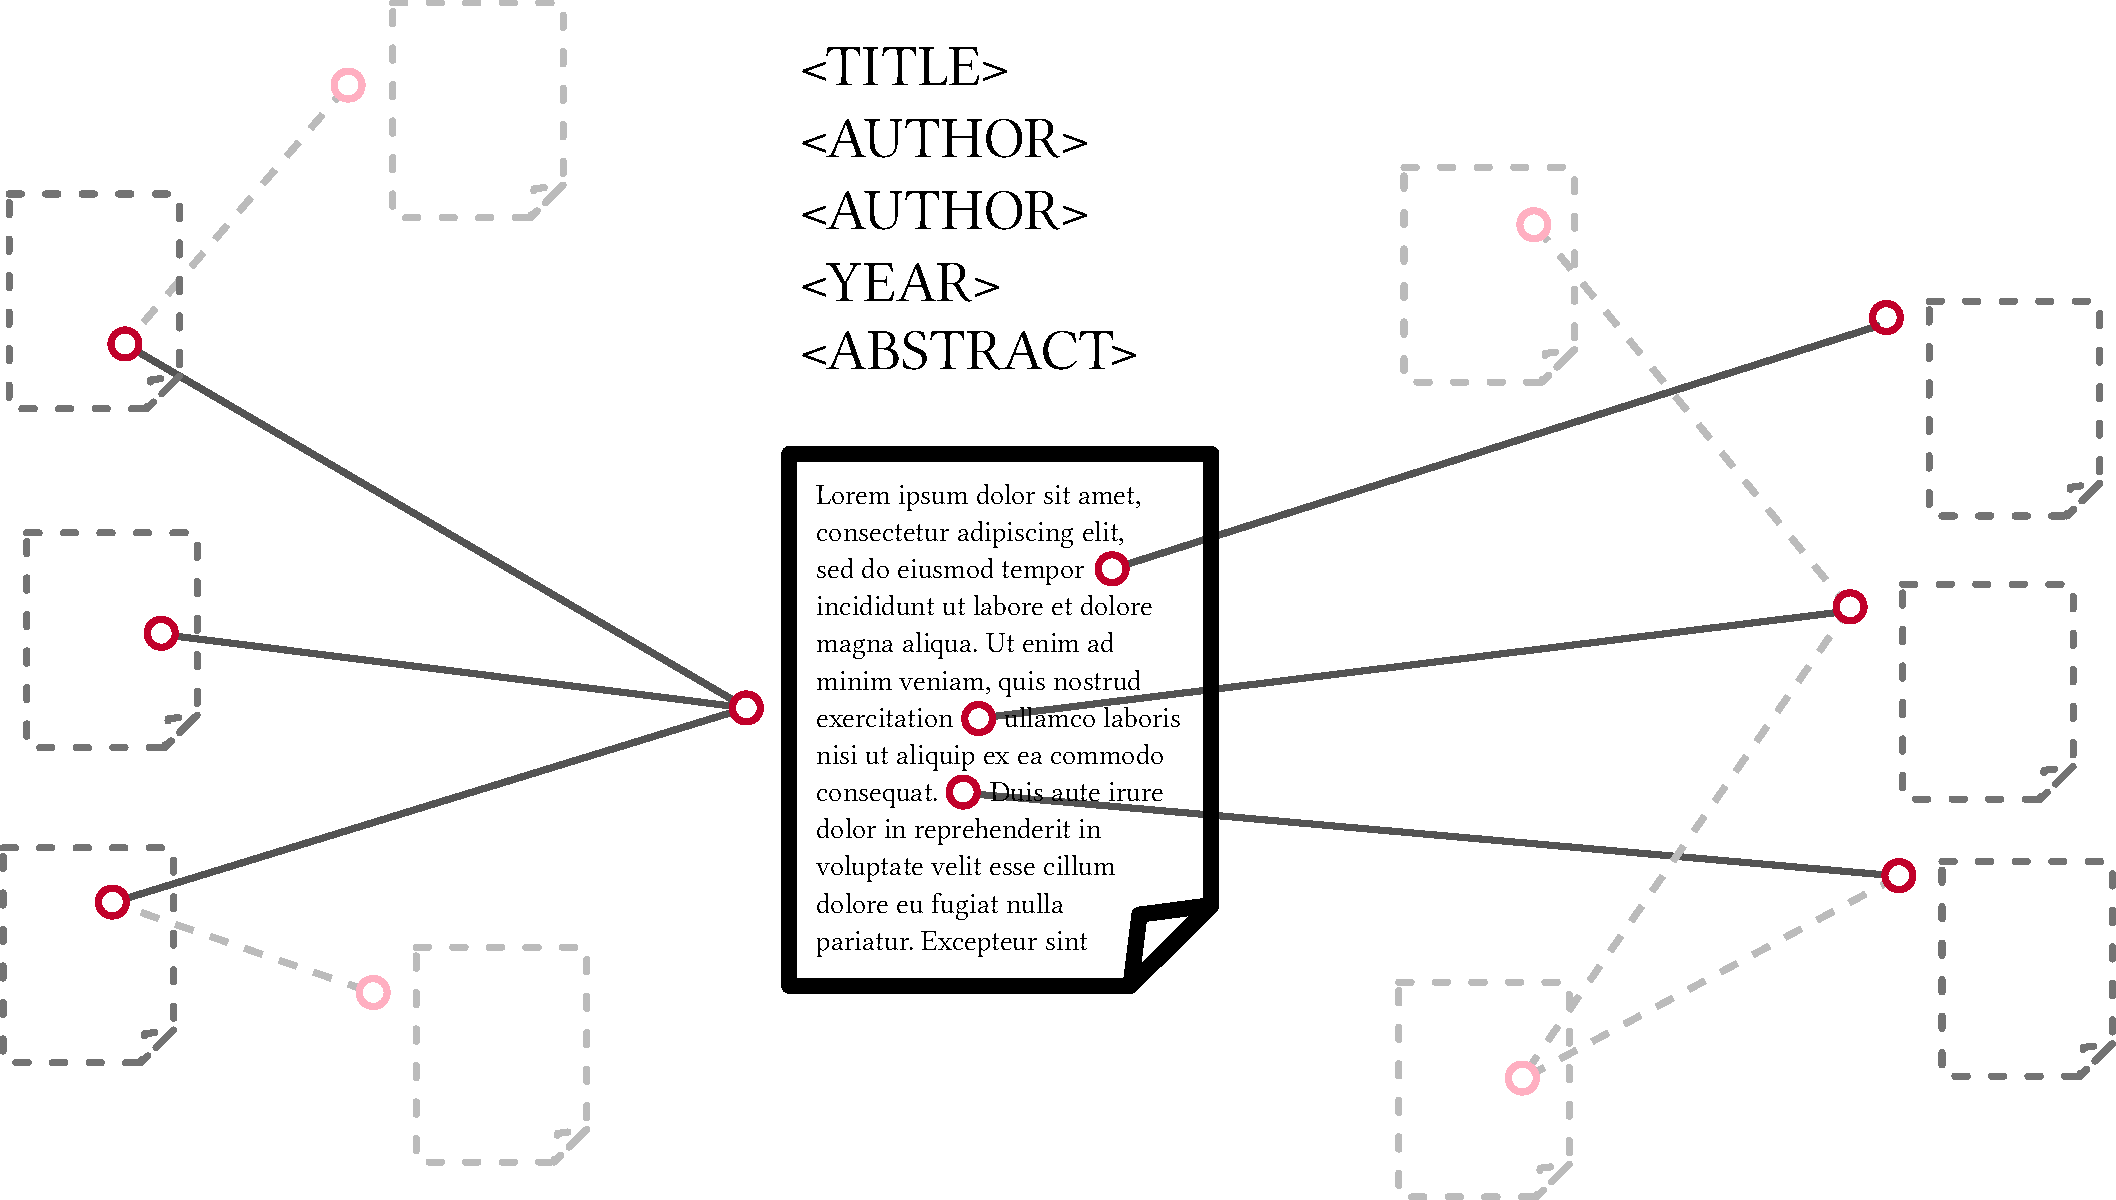
\includegraphics[width=0.8\textwidth]{figures/background/document_rich_view.pdf}
  \caption{Schematic view on a document, its metadata and embedding in the citation graph.}
  \label{fig:docrichview}
\end{figure}

\begin{figure}[t]
  \centering
    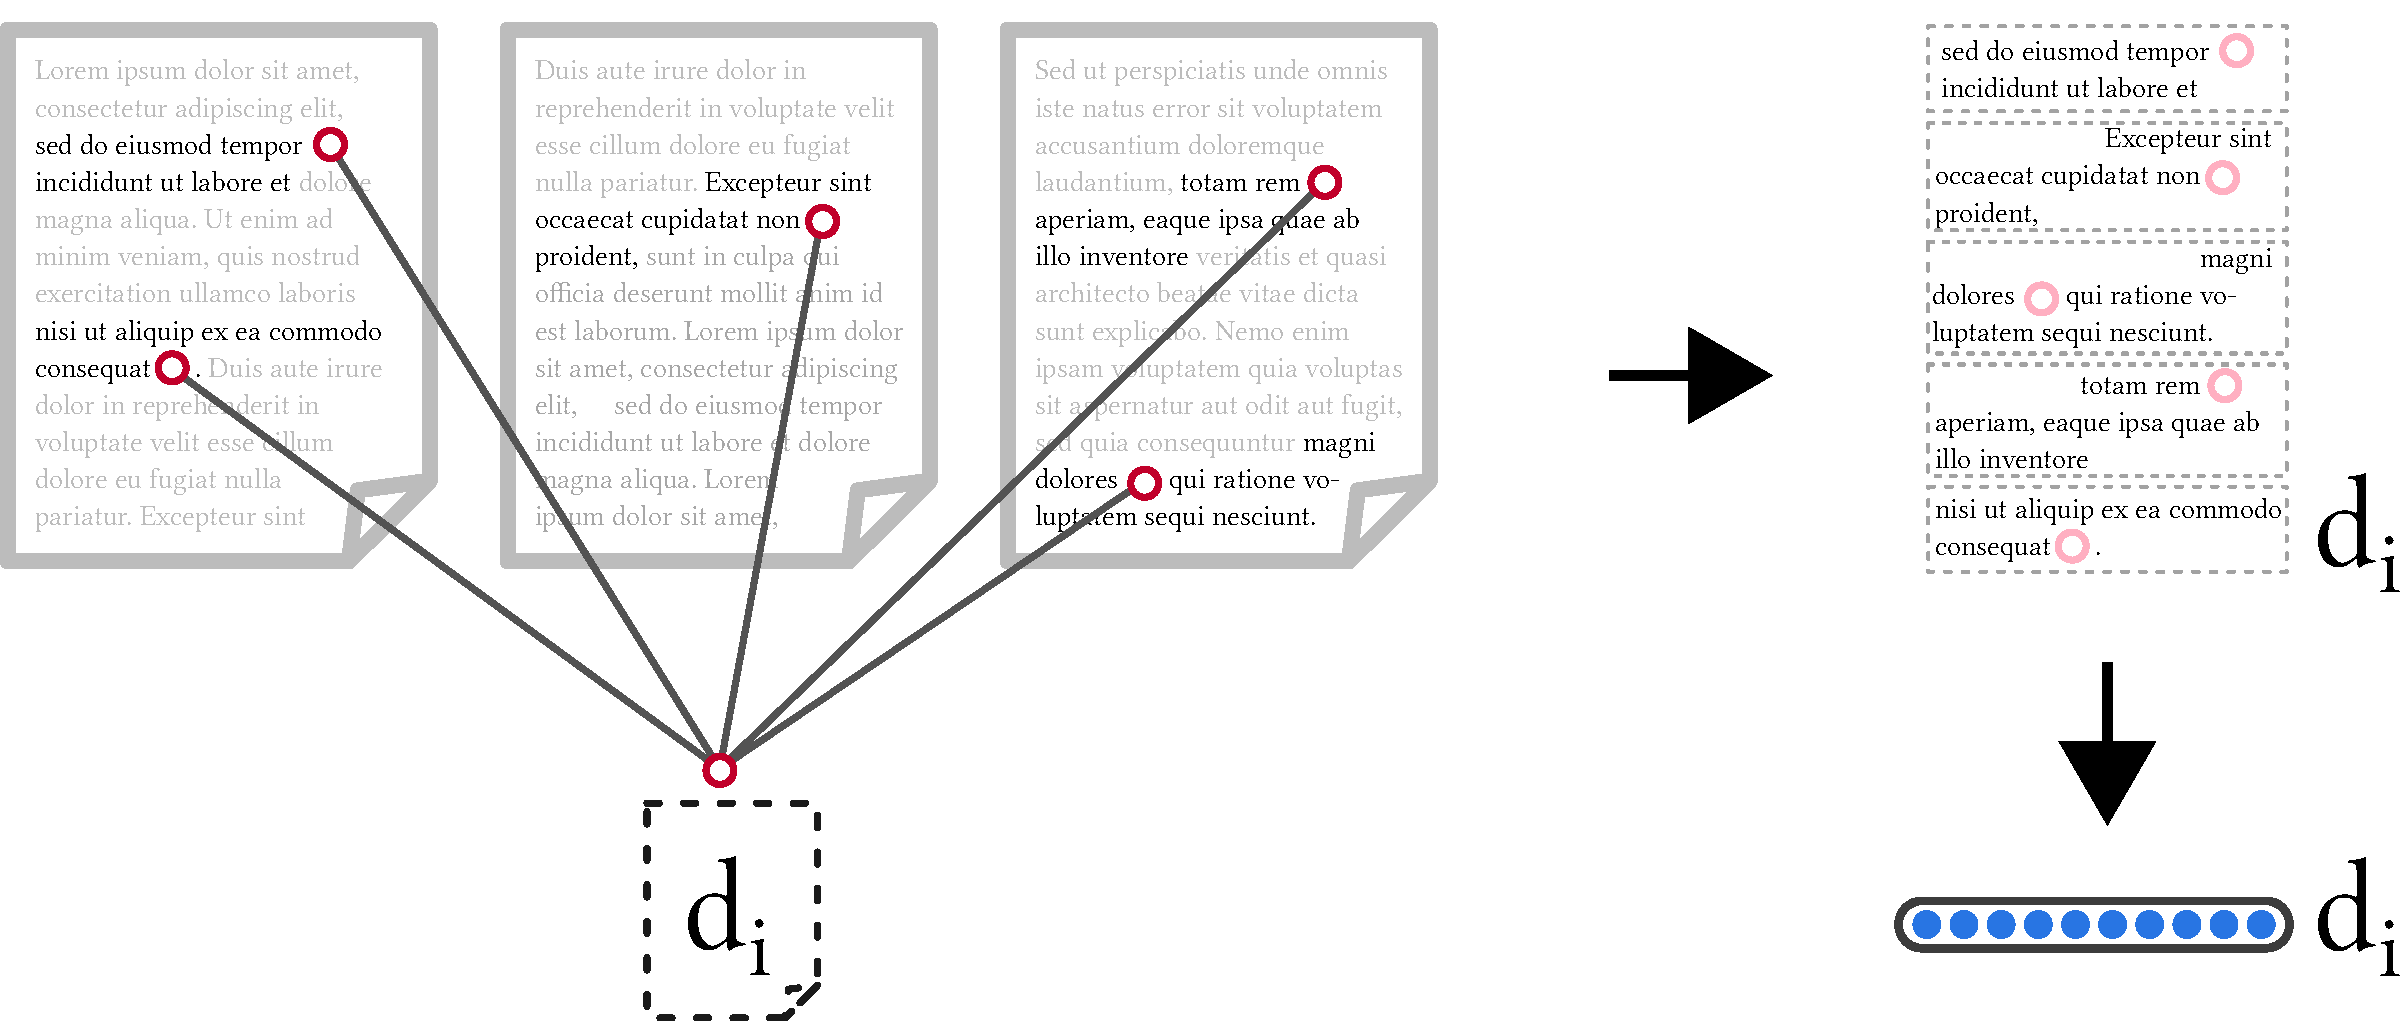
\includegraphics[width=\textwidth]{figures/background/document_context_view_withvec.pdf}
  \caption{Schematic visualization of a document's representation using citation contexts.}
  \label{fig:doccontview}
\end{figure}

As mentioned above, the focus in the case of citation recommendation lies on the candidate items---which are scientific publications. Figure~\ref{fig:docrichview} shows the types of information that are available to describe them. First and foremost each publication has, of course, its textual contents. Alongside this it is also part of a network of citations, meaning is has documents it is being cited by as well as documents it is citing. Lastly, there may also be metadata describing the document, such as the title, authors, year of publication etc. In order to study the viability of using explicit semantic representations of citation contexts for citation recommendation, without introducing any confounding variables, we will describe our documents \emph{only} by citation contexts. As citation contexts have been shown to contain information similar to and sometimes more extensive and focussed than abstracts~\cite{Elkiss2008}, we can expect decent recommendation results even though we're not taking any metadata associated with or textual content contained in the candidate documents into account. Figure~\ref{fig:doccontview} shows how a document representation can be generated from citation contexts. Document $d_i$ is cited by several other documents. By aggregating the contexts of these citations and deriving an abstract representation, $d_i$ can be represented by how it is being referenced in existing literature.
% Generating such representations of recommendation candidates is referred to as learning or training.

\begin{figure}[!b]
  \centering
    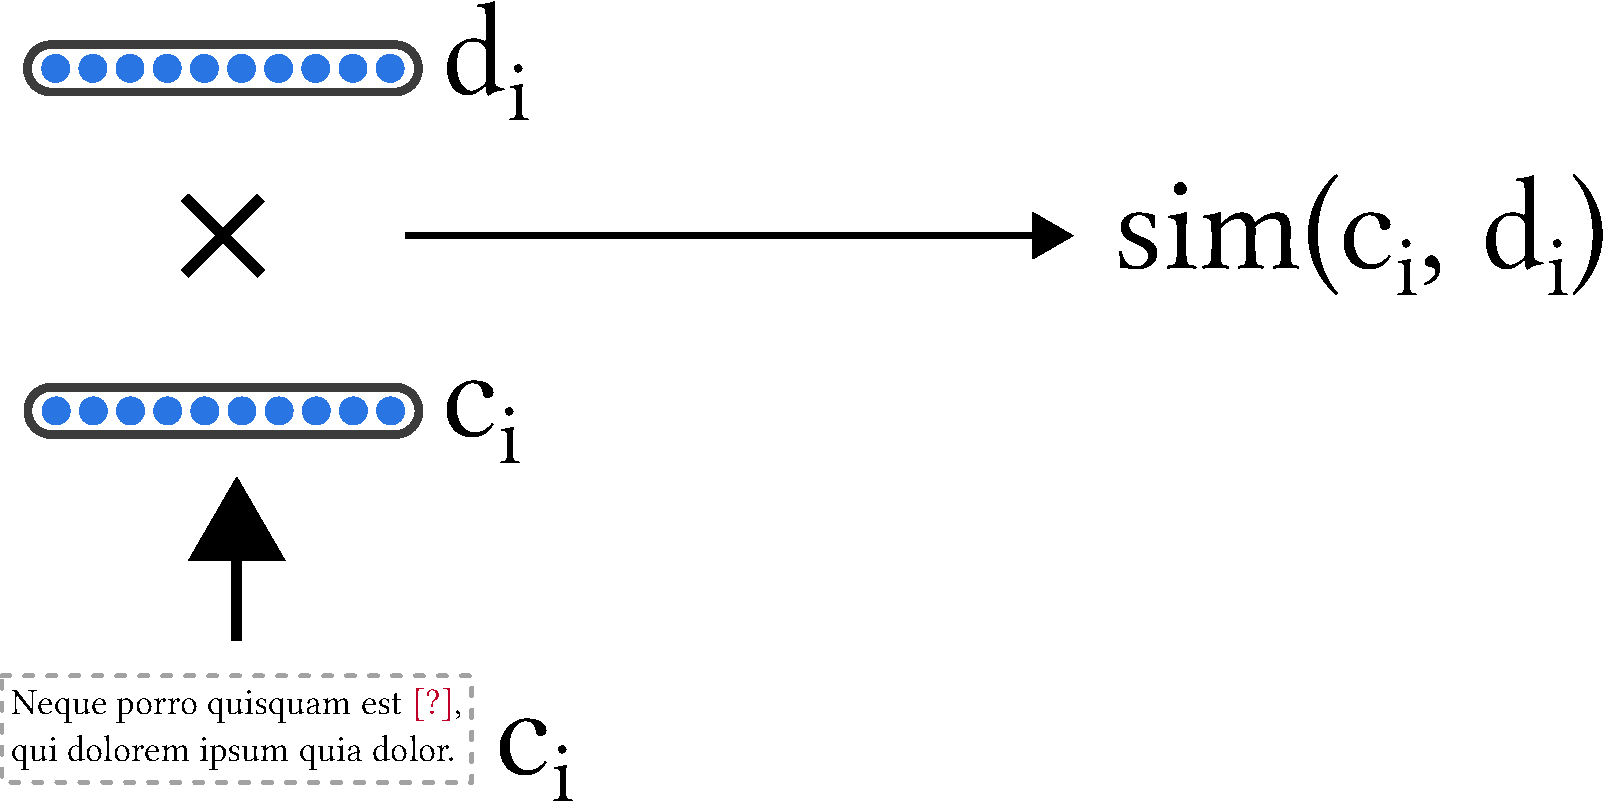
\includegraphics[width=0.7\textwidth]{figures/background/document_context_view_comparison.pdf}
  \caption{Schematic visualization of determining the similarity between an input citation contexts and a document representation.}
  \label{fig:doccomp}
\end{figure}

Recommendation itself is then done by taking a citation contexts $c_i$ as input, deriving an abstract representation in the same manner as was done for the aggregated contexts referencing a document, and then comparing the input's representation against those of all the documents. One such comparison is schematically depicted in Figure~\ref{fig:doccomp}. When every document---i.e., recommendation candidate---is associated with a similarity score, the system can output the most similar candidates as recommendations. With this, the overall picture looks as follows. The recommender system is trained on citation contexts, from which representations of the cited documents are learned. These documents are the publications the system is able to recommend. For a new context (without attached citation) given as input, the system identifies the documents most similar in the abstract representation space to the input and outputs these as recommendations.

\subsection{Evaluating citation recommendations}
Evaluation of recommender systems can be divided into three types, online evaluation, user study and offline evaluation. Online evaluation refers to monitoring naturally occurring user interaction with a system deployed online and drawing conclusions from metrics like click-through rates. User studies are conducted in a more controlled manner where users are aware of the evaluation and may be asked for explicit feedback on parts of the system. Offline evaluation differs from the other two types in that it does not directly involve human judgement. Rather, part of the data the system would, for online deployment, be trained on, is withheld and used as testing data. In doing this, past user judgement (like rating a movie or placing a citation) is used as a ground truth to test the system's output against. Because the human judgement is implicitly given within the data and can be processed automatically, offline evaluations can easily be performed on a large scale.~\cite{Aggarwal2016}

When recommending citations, abovementioned three types of evaluation can be realized as follows. Online evaluation can be performed by measuring which, if any, of the suggested publications a user actually inserts into their text. In a user study, participants can be asked to judge the relevance of recommended items while the system's input could be chosen by the user or given by the creators of the study. Lastly, offline evaluation as outlined above results in a re-prediction setting. That is, existing citation contexts are stripped of their citations, input into the system, and the resulting output compared to the original.

To aggregate relevance judgements of a large number of recommendations into a single number in order to compare different approaches, metrics are necessary. We use Recall, MRR, MAP and NDCG measured at different cut-off values. A cut-off, often denoted as \emph{Metric@}$k$, means only taking the top $k$ recommendations into consideration. This is done because, realistically, a user will not go through a list of hundreds of suggested items, but only look at the top three, five or maybe ten. Recall, MRR, MAP and NDCG with a cut-off $k$ can be defined as follows (see \cite{Aggarwal2016} for a more detailed, general discussion of these metrics):

Let $\mathcal{R} = r_1,r_2, ..., r_n$ be the ordered list of recommended items (highest to lowest) and ${\mathit{rel}(r_i)\in[0, 1]}$ denote the relevance of item $r_i$ at rank $i$. Furthermore let ${\mathcal{R}_{rel}=\{r_i|\mathit{rel}(r_i)=1\}}$ be the set of relevant items in an evaluation where $\mathit{rel}(r_i)\in\{0,1\}$---that is, an item is either relevant or not, with no partial relevance in between. Note that in a re-prediction setting as described above, $|\mathcal{R}_{rel}|=1$.

\paragraph{Recall} measures the fraction of the number of relevant items that was retrieved. If a cut-off $k$ is applied, the fraction's denominator is the minimum of the number of relevant items and the cut-off value.\[ \mathit{Recall}@k = \frac{\sum\limits_{i=1}^{k} \mathit{rel}(r_i)}{\mathit{min}(|\mathcal{R}_{rel}|,k)} \] For an evaluation with multiple test inputs, the mean over all Recall@k values is taken.

\paragraph{MRR} (mean reciprocal rank) is a metric often used when there is just one relevant item (e.g. re-prediction of a citation) or (when there are multiple relevant items) defined to just consider the first one. It takes into account the position of a recommended item through dividing its relevance by its rank.\[ \mathit{MRR}@k = \frac{\sum\limits_{i=1}^{k} \frac{\mathit{rel}(r_i)}{i}}{\mathit{min}(|\mathcal{R}_{rel}|,k)} \] Again, when evaluating over multiple test inputs, the mean over all MRR@k values is calculated.

\paragraph{MAP} (mean average precision) is the mean of average precision (\textbf{AP}) values of multiple queries. AP measures the average of all precision values at the ranks where relevant items are found. To define this, let $\rho(k)$ denote the number of relevant items within the first $k$ ranks. AP is then defined as \[ \mathit{AP}@k = \frac{\sum\limits_{i=1}^{k} \frac{\rho(i)}{i}\times\mathit{rel}(r_i)}{\mathit{max}(\rho(k), 1)} \] where $\mathit{rel}(r_i)\in\{0,1\}$. The value of MAP@k is the mean AP@k over all evaluated queries.

\paragraph{NDCG} (normalised discounted cumulative gain) is a metric compatible with non-binary relevance values that, similar to MAP, places higher weight on top ranks. It is calculated as the DCG (discounted cumulative gain) over the IDCG (ideal discounted cumulative gain)
 \[ \mathit{NDCG}@k = \frac{DCG@k}{IDCG@k} \]
where DCG is a sum of discounted relevance values
 \[ \mathit{DCG}@k = \sum\limits_{i=1}^{k} \frac{2^{\mathit{rel}(r_i)}-1}{\mathit{log}_2(i+1)} \]
and IDCG is a normalization factor to get values between zero and one, derived from an ideal recommendation $\mathcal{R}_{\mathit{ideal}}$ in which all items are ordered from the most relevant to the least
 \[ \mathit{IDCG}@k = \sum\limits_{r\in\mathcal{R}_{\mathit{ideal}}}\frac{2^{\mathit{rel}(r)}-1}{\mathit{log}_2(i+1)} \]
Likewise to the other metrics, the mean is calculated when evaluating over a set of test inputs.

    \chapter{Data set}\label{chap:dataset}
Recommender systems rely on data for their development, training and evaluation. It is therefore important to properly assess potential data sets in terms of their strengths and shortcomings---especially with regards to the task at hand. In citation recommendation, the goal is to identify papers relevant to a user input. Because of the large amount of available research, this means a recommender has to be able to find relevant publications in a large set of possible candidates in order to be considered fit for the task. As a comsequence, evaluation results are likely to be more meaningful when a large data set is used. Apart from the size, the quality of data is also crucial. For local citation recommendation this means that a clean citation context, precise position of citaiton markers and valid citation information are desirable. With these criteria in mind we assessed existing data sets and come to the conclusion that, for the relatively new task of local citation recommendation, the creation of a dedicated data set will bring considerable benefits.

The following sections describe the details of our assessment as well as the creation process and evaluation of our new data set.

\section{Existing data sets}

\begin{table}
\centering
    \caption[Overview of existing data sets.]{Overview of existing data sets.\\Listed are the number of papers, nature of citation contexts, covered disciplices of citing papers and the type of global reference identifiers.\\(\emph{extractable*} is to indicate that extraction might be error-prone due to papers only being available as in PDF format.)}
    \label{tab:datasets}
\begin{center}
    % \caption{Overview of existing data sets.}
    % \label{tab:existing-data-sets}
    \begin{tabular}{lllll}
    \toprule
    Data set & \#Papers & Cit. context & Disciplines & Ref. IDs \\
    \midrule
    CiteSeerX~\cite{Caragea2014} / RefSeer~\cite{Huang2014} & 5M & 400 chars & (unrestricted) & internal \\
    PubMed Central OAS\footnote{\url{https://www.ncbi.nlm.nih.gov/pmc/tools/openftlist/}} & 2.3M & extractable & Biomed./Life Sci. & mixed \\
    arXiv CS~\cite{Faerber2018} &  90K & 1 sentence & CS & DBLP \\
    Scholarly~\cite{Sugiyama2013}  & 100K & extractable* & CS & - \\
    ACL-AAN  & 18K & extractable* & CS/Comp. Ling. & -  \\ % \cite{Radev2013}
    ACL-ARC  & 11K & extractable* & CS/Comp. Ling. & - \\ % \cite{Bird2008ACLARC}
    \bottomrule
    \end{tabular}
\end{center}
\end{table}

Table~\ref{tab:datasets} gives an overview of relevant existing data sets. While various recommendation domains have established quasi standard data sets, this is not yet the case in citation recommendation. CiteSeerX is currently the most used in the field~\cite{Beel2016}. It is comparatively large, but many approaches only use subsets and generate them with varying filtering criteria. It includes pre-extracted citation contexts of 400 characters in length, whereby references are resolved to an internal set of identifiers. Unfortunately there are several quality issues with the data set. The main ones being inaccurate citaion information, noisy citation contexts and cut off words at the borders of citation contexts~\cite{Roy2016}.

The PubMed Central Open Access Subset (PMC-OAS) is another large data set that has been used for citation based tasks~\cite{Duma2016,Gipp2015,Galke2018,Bhagavatula2018}. Contained publications are already processed and available in XML format. While the data set overall is comparatively clean, heterogeneous annotation of citations within the text and mixed usage of global reference identifiers (PubMed, MEDLINE, DOI, ...) make it difficult to retrieve high quality citation interlinkings of documents from the data set\footnote{To be more precise, the heterogeneity makes the usage of the data set \emph{as is} problematic. Resolving references retrospectively would be an option but comparatively challenging in the case of PubMed because of the frequent usage of special notation in publication titles; see also: \texttt{\url{http://www.sciplore.org/files/citrec/CITREC_Parser_Documentation.pdf}}}~\cite{Gipp2015}.

Consistent global reference identifiers are given in the arXiv CS data set in the form of DBLP IDs. Linking to an existing repository of publication (meta) data has the advantage that information about cited papers in readily available. The choice of DBLP restricts resolved references to the field of computer science though. Citations to, for example, publications in maths or statistics can not be resolved to a DBLP ID. A strength of the data set is that it was generated from \LaTeX{} source files, which makes it possible to get very clean data.

For the remainig the data sets---Scholarly, ACL-AAN and ACL-ARC---citing papers are only available in PDF format and references are not resolved. The two ACL sets have the additional drawback of being very small.

Above observations lead us to the conclusion that it would be worthwhile to tackle the creation of a data set that is large (in the order of CiteSeerX/RefSeer/PMC-OAS), clean (like the PMC-OAS and arXiv CS) and also offers consitent global reference IDs that don't restrict the data set to citations within the same discipline. The creation and evaluation of this data set is described in the following sections.

% TODO: mby add MAG use/analysis: \cite{Herrmannova2016,Paszcza2016,Hug2017}

% TODO: add: evaluation of reference string parsers\cite{Tkaczyk2018}, a dataset for reference string parsing\cite{Anzaroot2013}

\section{Data set creation}\label{sec:data-set-creation}
Scientific publications are usually distributed in formats targeted at human consumption (e.g. PDF) or, in cases like arXiv.org, also as source files \emph{for} the aforementioned (e.g. \LaTeX{} sources for generating PDFs). Citation-based tasks, such as local citation recommendation, in contrast, require automated processing of the publications' textual contents as well as the documents' interlinking through citations. The creation of a data set for such tasks therefore encompasses two main steps: extraction of plain text and resolution of references. In the following we will describe how we approached these two steps using arXiv publication sources and the Microsoft Academic Graph (MAG)~\cite{Sinha2015}.

\subsection{Used data sets}

The following two resources are the basis of the data set creation process.

\paragraph{arXiv.org} hosts over 1.4 million submissions from August 1991 onward~\cite{Ginsparg1994}. They are available not only as PDF, but (in most cases) also as \LaTeX{} source files. The discipline most prominently represented is physics, followed by mathematics, with computer science seeing a continued increase in percentage of submissions ranking third (see Fig.~\ref{fig:sankey}). The availability of \LaTeX{} sources makes arXiv submissions particularly well suited for extracting high quality plain text and accurate citation information. So much so, that it has been used to generate ground truths for the evaluation of PDF to text conversion tools~\cite{Bast2017}. Approaches to automatically extract citation interlinks from arXiv sources by parsing \LaTeX{} files have existed for over 20 years \cite{Nanba1998}. Nevertheless we are not aware of any existing data sets for citation based tasks generated from the whole of arXiv.

\paragraph{Microsoft Academic Graph (MAG)} is a very large\footnote{At the time of writing the MAG contains data on over 200 million publications.}, automatically generated data set on publications, related entities (authors, venues, etc.) and their interconnections through citation. While citation contexts are available to some degree, full text documents are not. The size of the MAG makes it a good target for matching reference items against it, especially given that arXiv spans several fields of study.

\subsection{Pipeline overview}

As depicted in Figure~\ref{fig:datagen}, we start out with arXiv sources to create the data set. From these we generate, per publication, a plain text file with the document's textual contents and a set of database entries reflecting the document's reference section. Association between reference items and citations in the text are preserved by placing citation markers in the text. In a second step, we then iterate through all reference items in the database and match them against paper metadata records in the MAG. The result of this process are MAG paper records associated with one or more reference items, that in turn are associated with citation contexts in the plain text files. In other words, we end up with cited documents described by their MAG metadata and a distributed description of the document, consisting of citation contexts over many citing documents.

\begin{figure}
  \centering
    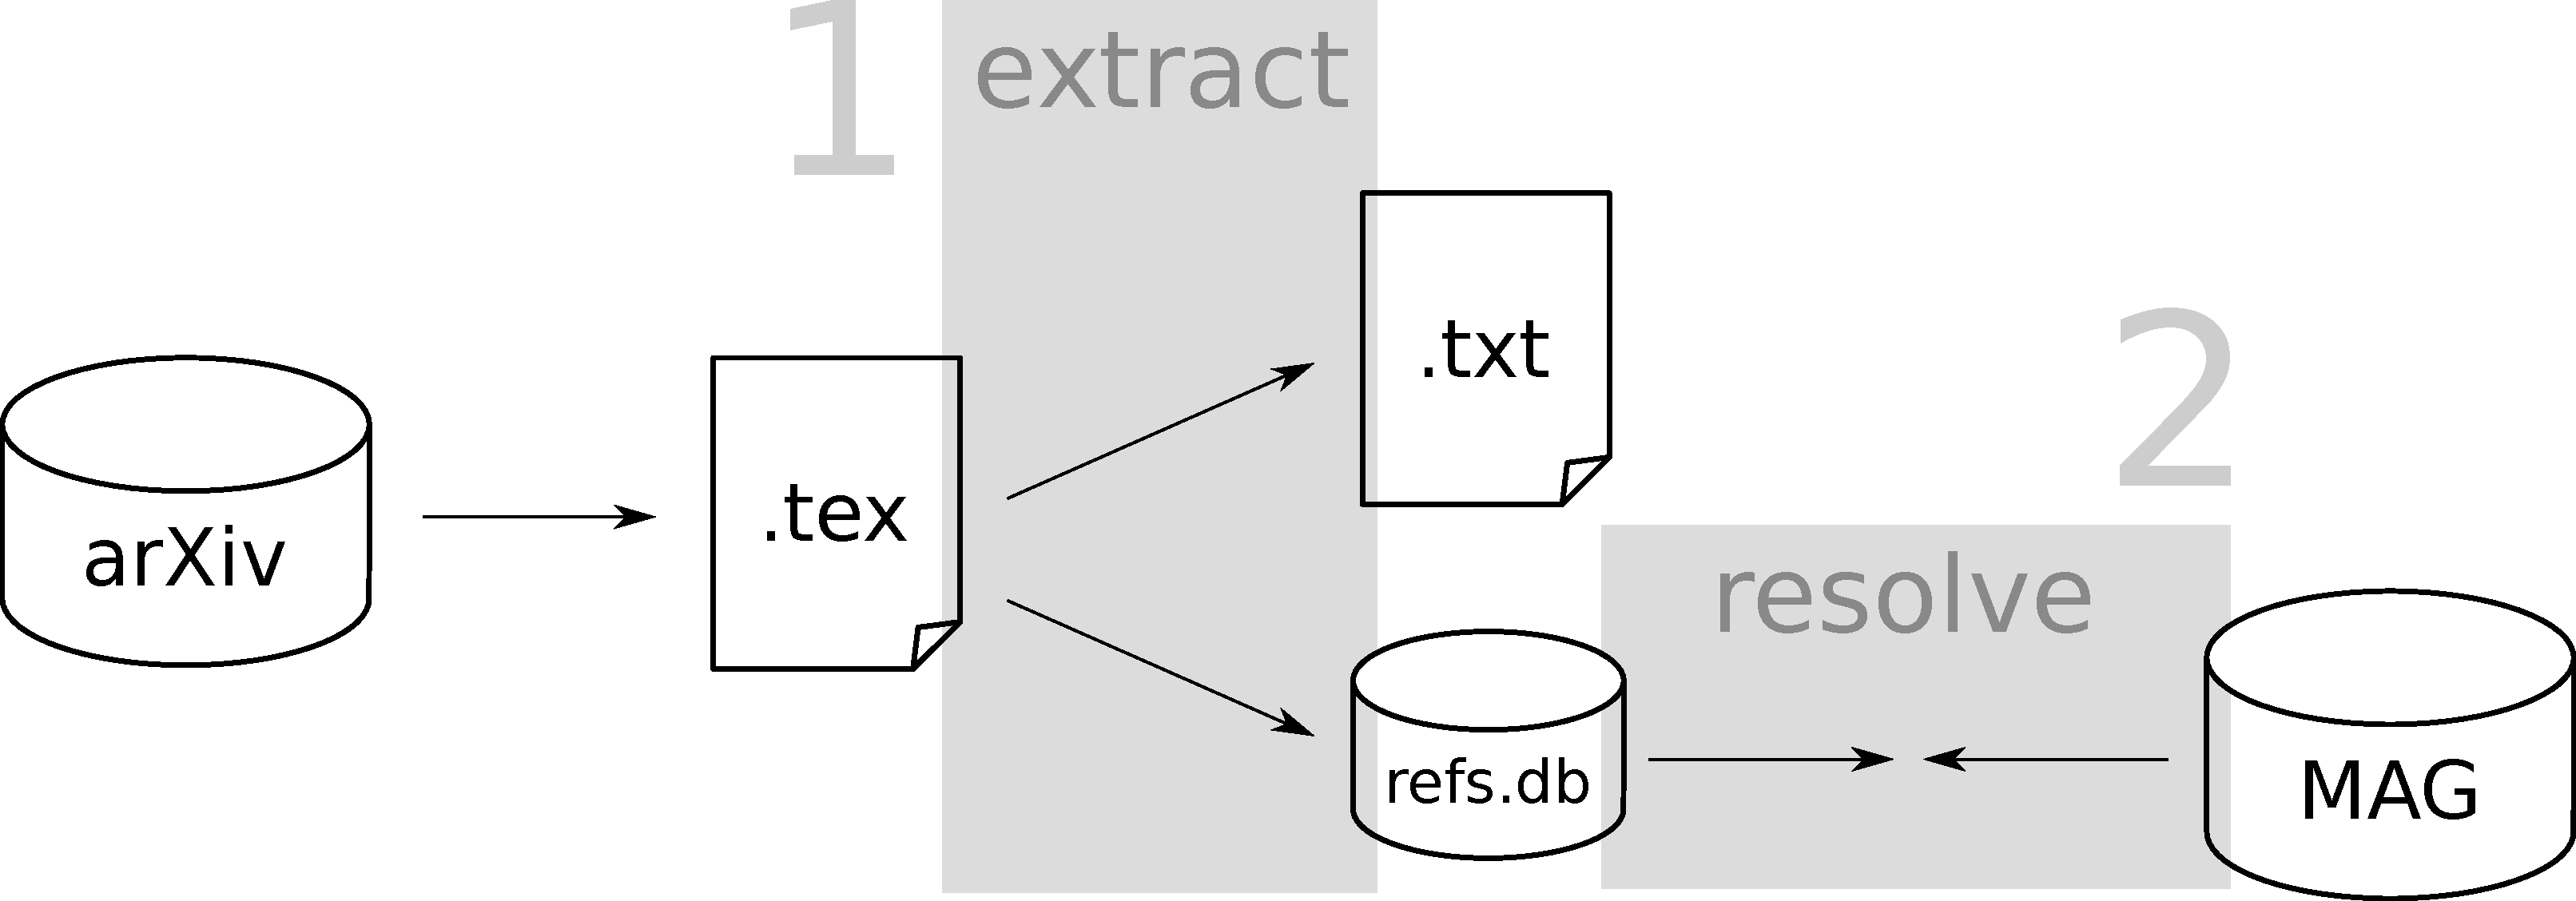
\includegraphics[scale=0.2]{figures/dataset/data_set_generation_schema.pdf}
  \caption{Schematic representation of the data set generation process.}
  \label{fig:datagen}
\end{figure}

\subsection{\LaTeX{} Parsing}
In the following we will describe the tools considered for parsing \LaTeX{}, the challenges we faced in general and with regard to arXiv sources in particular, and our resulting approach.

\subsubsection{Tools}

\begin{table}[t]
\centering
  \caption{Comparison of tools for parsing \LaTeX{}.}
  \label{tbl:tools}
\begin{tabular}{llll}
\toprule
    Tool & Output & Robust & Usable w/o modification \\
   \midrule
    plastex\footnote{\url{https://github.com/tiarno/plastex}} & DOM & no & yes\\
    TexSoup\footnote{\url{https://github.com/alvinwan/texsoup}} & document tree & no & yes\\
    opendetex\footnote{\url{https://github.com/pkubowicz/opendetex}}/detex\footnote{\url{https://www.freebsd.org/cgi/man.cgi?query=detex}} & plain text & no & yes\\
    GrabCite\cite{Faerber2018} & plain\hphantom{ }text\hphantom{ }+ resolved ref. & yes & no\\
    LaTeXML\footnote{\url{https://github.com/brucemiller/LaTeXML}} & XML & yes & yes\\
    Tralics\footnote{\url{https://www-sop.inria.fr/marelle/tralics/}} & XML & yes & yes\\
  \bottomrule
\end{tabular}
\end{table}

We took several tools for the conversion from \LaTeX{} to plain text or to intermediate formats into consideration and evaluated them. Table \ref{tbl:tools} gives an overview of our results. Half of the tools failed to produce any output for a large amount of arXiv submissions we used as test input and were therefore deemed not robust enough. \textit{GrabCite} is able to parse 78.5\% of arXiv CS submissions but integrates resolving references against DBLP into the parsing process and therefore would require significant modification to fit our system architecture. \textit{LaTeXML} and \textit{Tralics} are both robust and can be used as \LaTeX{} conversion tools as is. On subsequent tests we note that \textit{LaTeXML} needs on average 7.7 seconds (3.3 if formula environments are heuristically removed beforehand) to parse an arXiv submission while \textit{Tralics} needs 0.09. Because the quality of their output seemed comparable we chose to use \textit{Tralics}.

\subsubsection{Challenges}
Apart from the general difficulty of parsing \LaTeX{} due to its feature richness and people's free-spirited use of it, we especially note difficulty in dealing with extra packages not included in submissions' sources\footnote{arXiv.org specifically suggest the omission of such (see \texttt{\url{https://arxiv.org/help/submit\_tex\#wegotem}})}. While \textit{Tralics} is supposed to for example deal with \textit{natbib} citations\footnote{See \texttt{\url{https://www-sop.inria.fr/marelle/tralics/packages.html\#natbib}}}, normalization of such citations lead to a decrease of citation markers not being able to be matched to their reference item from 30\% to 5\% in a sample of 565,613 citations we tested.

\subsubsection{Resulting approach}
Our \LaTeX{} parsing solution consists of two steps. First, we flatten each arXiv submission's sources to a single \LaTeX{} file using \textit{latexpand}\footnote{See \url{https://ctan.org/pkg/latexpand}}\textsuperscript{,}\footnote{We also tested flatex (\url{https://ctan.org/pkg/flatex}) and flap (\url{https://github.com/fchauvel/flap}) but got the best results with \texttt{latexpand}.} and normalize \texttt{\textbackslash cite} commands to prevent parsing problems later on. In the second step, we then generate an XML representation of the \LaTeX{} document using \textit{Tralics}, replace formulas, figures, tables and non citation references with replacement tokens and extract the plain text. Furthermore, each reference item is assigned a unique identifier, its text is stored in a database and corresponding citation markers are placed in the plain text.

\subsection{Reference resolution}\label{sec:refresol}
Resolving references to globally consistent identifiers (e.g. detecting that the references (1), (2), and (3) in Listing~\ref{lst:refitems} all reference the same document) is a challenging and still unsolved task~\cite{Nasar2018}. Given it is, by itself, the most distinctive part of a publication, we base our reference resolution on the title of the cited work and use other pieces of information (e.g., authors' names) only in secondary steps. In the following we will describe the challenges we faced, matching arXiv.org submissions' reference items against MAG paper records and how we approached the task.

\begin{lstlisting}[caption={Examples of reference items.},label={lst:refitems}]
(1) V. N. Senoguz and Q. Shafi, arXiv:hep-ph/0412102
(2) V.N. Senoguz and Q. Shafi, Phys. Rev. D 71 (2005) 043514.
(3) V. N. Şenoğuz and Q. Shafi, ``Reheat temperature in supersymmetric hybrid inflation models,'' Phys. Rev. D 71, 043514 (2005) [hep-ph/0412102].
(4) V.Sauli, JHEP 02, 001 (2003).
(5) Aaij, Roel, et al. "Search for the $B^{0}_{s} \to \eta^{\prime}\phi$ decay" Journal of High Energy Physics 2017.5 (2017): 158.
(6) According to the numerous discussions with my colleagues <removed> and <removed> an experimental verification of our theoretical predictions is feasible.
\end{lstlisting} % (*$B^{0}_{s} \to \eta^{\prime}\phi$*)

\subsubsection{Challenges}
Reference resolution can be challenging when reference items contain only minimal amounts of information, when formulas are used in titles or when they refer to non publications (e.g., Listing~\ref{lst:refitems} (4)-(6)). A further problem we encountered was noise in the MAG. Our mechanism matched 13,041 reference items like \texttt{K. Kondo, hep-th/0303251.} and \texttt{T. Heinzl, hep-th/9812190.} to a MAG paper with the title \textit{``hep-th.''} with one of the author's names being \textit{``He''} (paper ID \texttt{2811252340}).

\subsubsection{Resulting approach}
Our reference resolution procedure can be broken down in two steps: title identification and matching. If possible, title identification is done by arXiv ID or DOI (where we retrieve the title from an arXiv metadata dump or via crossref.org\footnote{See \url{https://www.crossref.org/}}); otherwise we use Neural ParsCit~\cite{Animesh2018}. The identified title is matched against the normalized titles of all publications in the MAG. Resulting candidates are considered, if at least one of the author's names is present in the reference string. If multiple candidates remain, we judge by the citation count given in the MAG. The last step particularly helped mitigate rouge almost-duplicate entries in the MAG that often have few to no citations.

\subsection{Result format}
Listing \ref{lst:formatall} shows some example content from the data set. While the data set in and of itself consists of plain text files and a references database, citation contexts of successfully resolved references are straightforward to extract and use as input for a recommender. The bottom part of Listing~\ref{lst:formatall} shows an example of a 3 sentence context with \texttt{cited doc MAG ID},\hphantom{n}\texttt{MAG IDs of adjacent citations},\hphantom{n}\texttt{citing doc arXiv ID} and \texttt{text} in a CSV format.

\begin{lstlisting}[caption={Excerpts from (top to bottom) a plain text file, corresponding data base entries in the references DB, entries in the MAG and extracted citation context CSV.},label={lst:formatall}]
It has over 79 million images stored at the resolution of FORMULA . Each image is labeled with one of the 75,062 non-abstract nouns in English, as listed in the Wordnet{{cite:9ad20b7d-87d1-47f5-aeed-10a1cf89a2e2}}{{cite: 298db7f5-9ebb-4e98-9ecf-0bdda28a42cb}} lexical database.

[uuid]         [in_doc]   [mag_id]    [reference_string]
9ad20b7d-87d1  1412.3684  2081580037  George A. Miller (1995). WordNe
-47f5-aeed-..                         t: A Lexical Database for Eng..
298db7f5-9ebb  1412.3684  2038721957  Christiane Fellbaum (1998), ""W
-4e98-9ecf-..                         ordNet: An Electronic Lexical..

[paperid]   [originaltitle]                           [publisher]  ...
2038721957  WordNet : an electronic lexical database  MIT Press    ...
2081580037  WordNet: a lexical database for English   ACM          ...

2038721957|2081580037|1412.3684|It has over 79 million images stored at the resolution of FORMULA . Each image is labeled with one of the 75,062 non-abstract nouns in English, as listed in the Wordnet CIT MAINCIT lexical database. It has been noted that many of the labels are not reliable CIT .
\end{lstlisting}

\section{Evaluation of reference resolution}
To evaluate the quality of our reference resolution results, we take a random sample of 300 matched reference items and manually check if the correct record in the MAG was identified by our method. Given the 300 items, we obtained 3 errors, giving us an accuracy estimate of 96\% at the worst, as shown in Table~\ref{tbl:confvals}.

\begin{table}[h]
  \caption[Confidence intervals for a sample size of 300 with 297 positive results.]{Confidence intervals for a sample size of 300 with 297 positive results as given by Wilson score interval and Jeffreys interval \cite{Brown2001}.}
  \label{tbl:confvals}
  \centering
\begin{tabular}{c@{\hspace{0.1in}}c@{\hspace{0.1in}}c@{\hspace{0.1in}}c}
\toprule
    Confidence level & Method & Lower limit & Upper limit \\\noalign{\smallskip}
\midrule
    0.99 & Wilson & 0.9613 & 0.9975 \\\noalign{\smallskip}
    \ & Jeffreys & 0.9666 & 0.9983 \\\noalign{\smallskip}
    \hline\noalign{\smallskip}
    0.95 & Wilson & 0.9710 & 0.9966 \\\noalign{\smallskip}
    \ & Jeffreys & 0.9736 & 0.9972 \\\noalign{\smallskip}
    \bottomrule
\end{tabular}
\end{table}

The three incorrectly identified references were as follows (MAG IDs in square brackets):
\begin{enumerate}
    \item \emph{``Eddy, J.A.: 1983, The maunder minimum - a reappraisal. Solar Phys. 89, 195. ADS.''}
    \begin{itemize}
        \item matched: [\texttt{2024069573}]\\\emph{``The Maunder Minimum''} (John A. Eddy; 1976)
        \item correct: [\texttt{2080336740}]\\\emph{``The Maunder Minimum: A reappraisal''} (John A. Eddy; 1983)
    \end{itemize}
    \item \emph{``J. Zhu, S. Rosset, T. Hastie, and R. Tibshirani. 1-norm support vector machines. In Advances in Neural Information Processing Systems (NIPS), volume 16, pages 49–56, 2004.''}
    \begin{itemize}
        \item matched: [\texttt{2249237221}]\\\emph{``Support Vector Machines''} (Gareth James, Daniela Witten, Trevor Hastie, Robert Tibshirani; 2013)
        \item correct: [\texttt{2130698119}]\\\emph{``1-norm Support Vector Machines''} (Ji Zhu, Saharon Rosset, Robert Tibshirani, Trevor J. Hastie; 2003)
    \end{itemize}
    \item \emph{``D. T. Limmer and D. Chandler. The putative liquid-liquid transition is a liquid-solid transition in atomistic models of water. The Journal of Chemical Physics, 135(13):134503, 2011.''}
    \begin{itemize}
        \item matched: [\texttt{2599889364}]\\\emph{``The Putative Liquid-Liquid Transition is a Liquid-Solid Transition in Atomistic Models of Water''} (David Chandler, David Limmer; 2013)
        \item correct: [\texttt{1977410206}]\\\emph{``The putative liquid-liquid transition is a liquid-solid transition in atomistic models of water. II''} (David T. Limmer, David Chandler; 2011)
    \end{itemize}
\end{enumerate}

In all three cases the misidentified document’s title is contained in the correct document’s title, and there is a large or complete author overlap between correct and actual match. This shows that authors sometimes title follow-up work very similarly, which leads to hard to distinguish cases. Another observation that can be made, is that longer titles are more distincitive. As certain publication titles might be sub-strings of of other publication's title, a matching mechanic should always try to first match a long title before trying shorter candidates. The full details of the evaluation can be found in Appendix~\ref{chap:matcheval}.

\section{Statistics and key figures}

\subsection{Creation process}
We used an arXiv source dump containing all submissions up until the end of 2017 (1,340,770 documents). 100,240 of these were only available in PDF format, leaving 1,240,530 sources. Our pipeline output 1,151,707 (92.8\%) plain text files, 1,018,976 (82.1\%) of which contained citation markers. The number of reference items identified is 35,053,329, for which 56,077,906 citation markers were placed within the plain text files. This first part of the process took 59 hours to run, unparallalized on a 8 core Intel Core i7-7700 3.60GHz machine with 60 GB of memory.

Of the 35,053,329 reference items, we were able to match 14,046,239 (40.07\%). For 33.14\% of the reference items we could neither find an arXiv ID or DOI, nor was Neural ParsCit able to identify a title. For the remaining 26.79\% a title was identified but could not be matched with the MAG. Of the matched 14 million items' titles, 50.67\% were identified via Neural ParsCit, 29.67\% by DOI and 19.66\% by arXiv ID. Of the identified DOIs 26.8\% were found as is while 73.2\% were heuristically determined\footnote{This was possible because the DOIs of articles in journals of the American Physical Society follow predictable patterns.}. The matching process took 103 hours, run in 10 parallel processes on a 64 core Intel Xeon Gold 6130 2.10GHz machine with 500 GB of memory.

\subsection{Resulting data set}
The resulting data set consists of \emph{2,343,585 cited papers, 926.644 citing papers, 13,303,373 references and 24,558,560 citation contexts}. Note that references with no citation markers (due to parsing errors) are not counted here.

Figure \ref{fig:numcitdoc} shows the number of citing documents for all cited documents. There is one document with close to 10,000 citations, another three with more than 5,000 and another ten with more than 3,000. 1,262,861 (53.89\%) of the documents have at least two citations, 547,036 (23.34\%) have at least five. The mean number of citations is 5.68 (SD 26.82). Figure \ref{fig:numcontref} shows the number of citation context per reference. 8,722,795 (65.57\%) references have only one citation context, the maximum is 278, the mean 1.85 (SD 2.02). This means a cited document is described by on average $1.85 \times 5.68 \approx 10.5$ citation contexts.

\begin{figure}
  \centering
  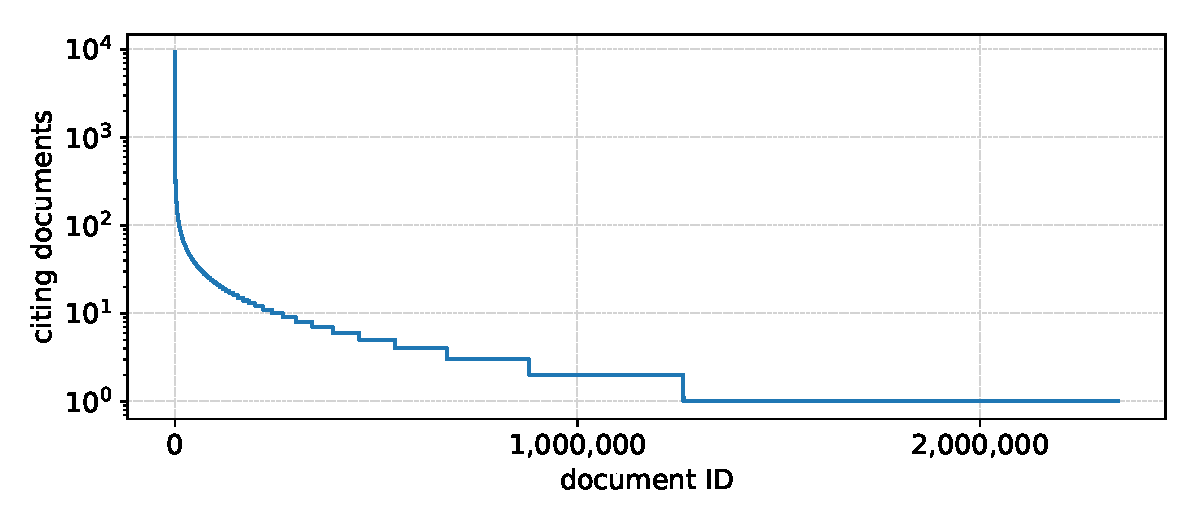
\includegraphics[width=\linewidth]{figures/dataset/citing_docs_per_cited_doc.pdf}
  \caption{Number of citing documents per cited document.}
  \label{fig:numcitdoc}
\end{figure}

\begin{figure}
  \centering
  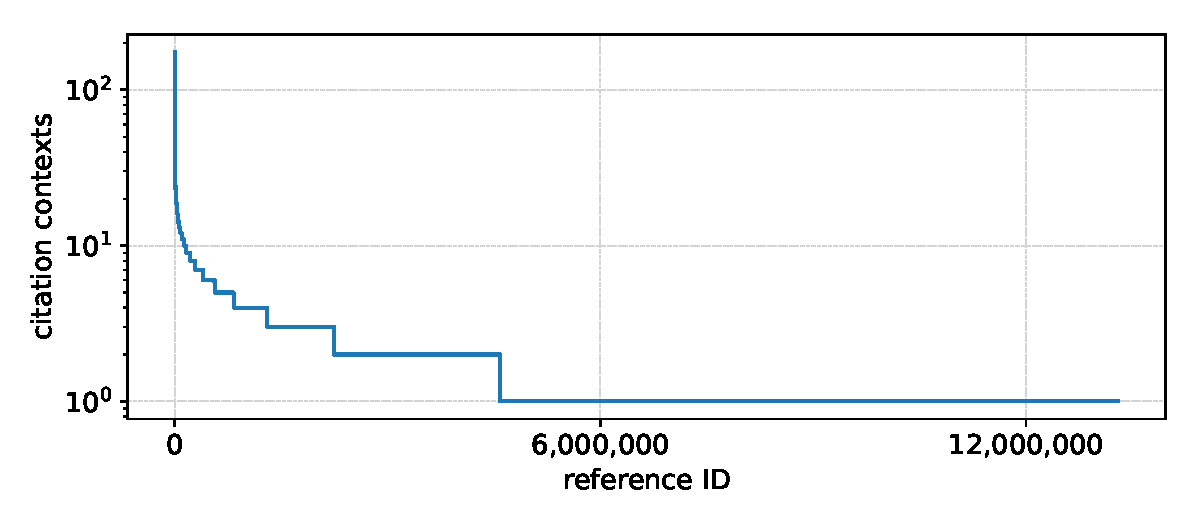
\includegraphics[width=\linewidth]{figures/dataset/citation_contexts_per_reference.pdf}
  \caption{Number of citation contexts per reference.}
  \label{fig:numcontref}
\end{figure}

Figure \ref{fig:sankey} depicts the flow of citations by field of study for all 13.3 million matched reference items. Fields of study with very small numbers of references are combined to \emph{other} for legibility reasons. For the citing document's side, these are economics, electrical engineering and systems science, quantitative biology, quantitative finance and statistics. Combined on the cited document's side are chemistry, biology, engineering, materials science, economics, geology, psychology, medicine, business, geography, sociology, political science, philosophy, environmental science and art. To no surprise, publications in each field are cited the most from within the field itself. Notable is, however, that the incoming citations in mathematics are the most varied (physics and computer science combined make up 38\% of the citations).

\begin{figure}
  \centering
    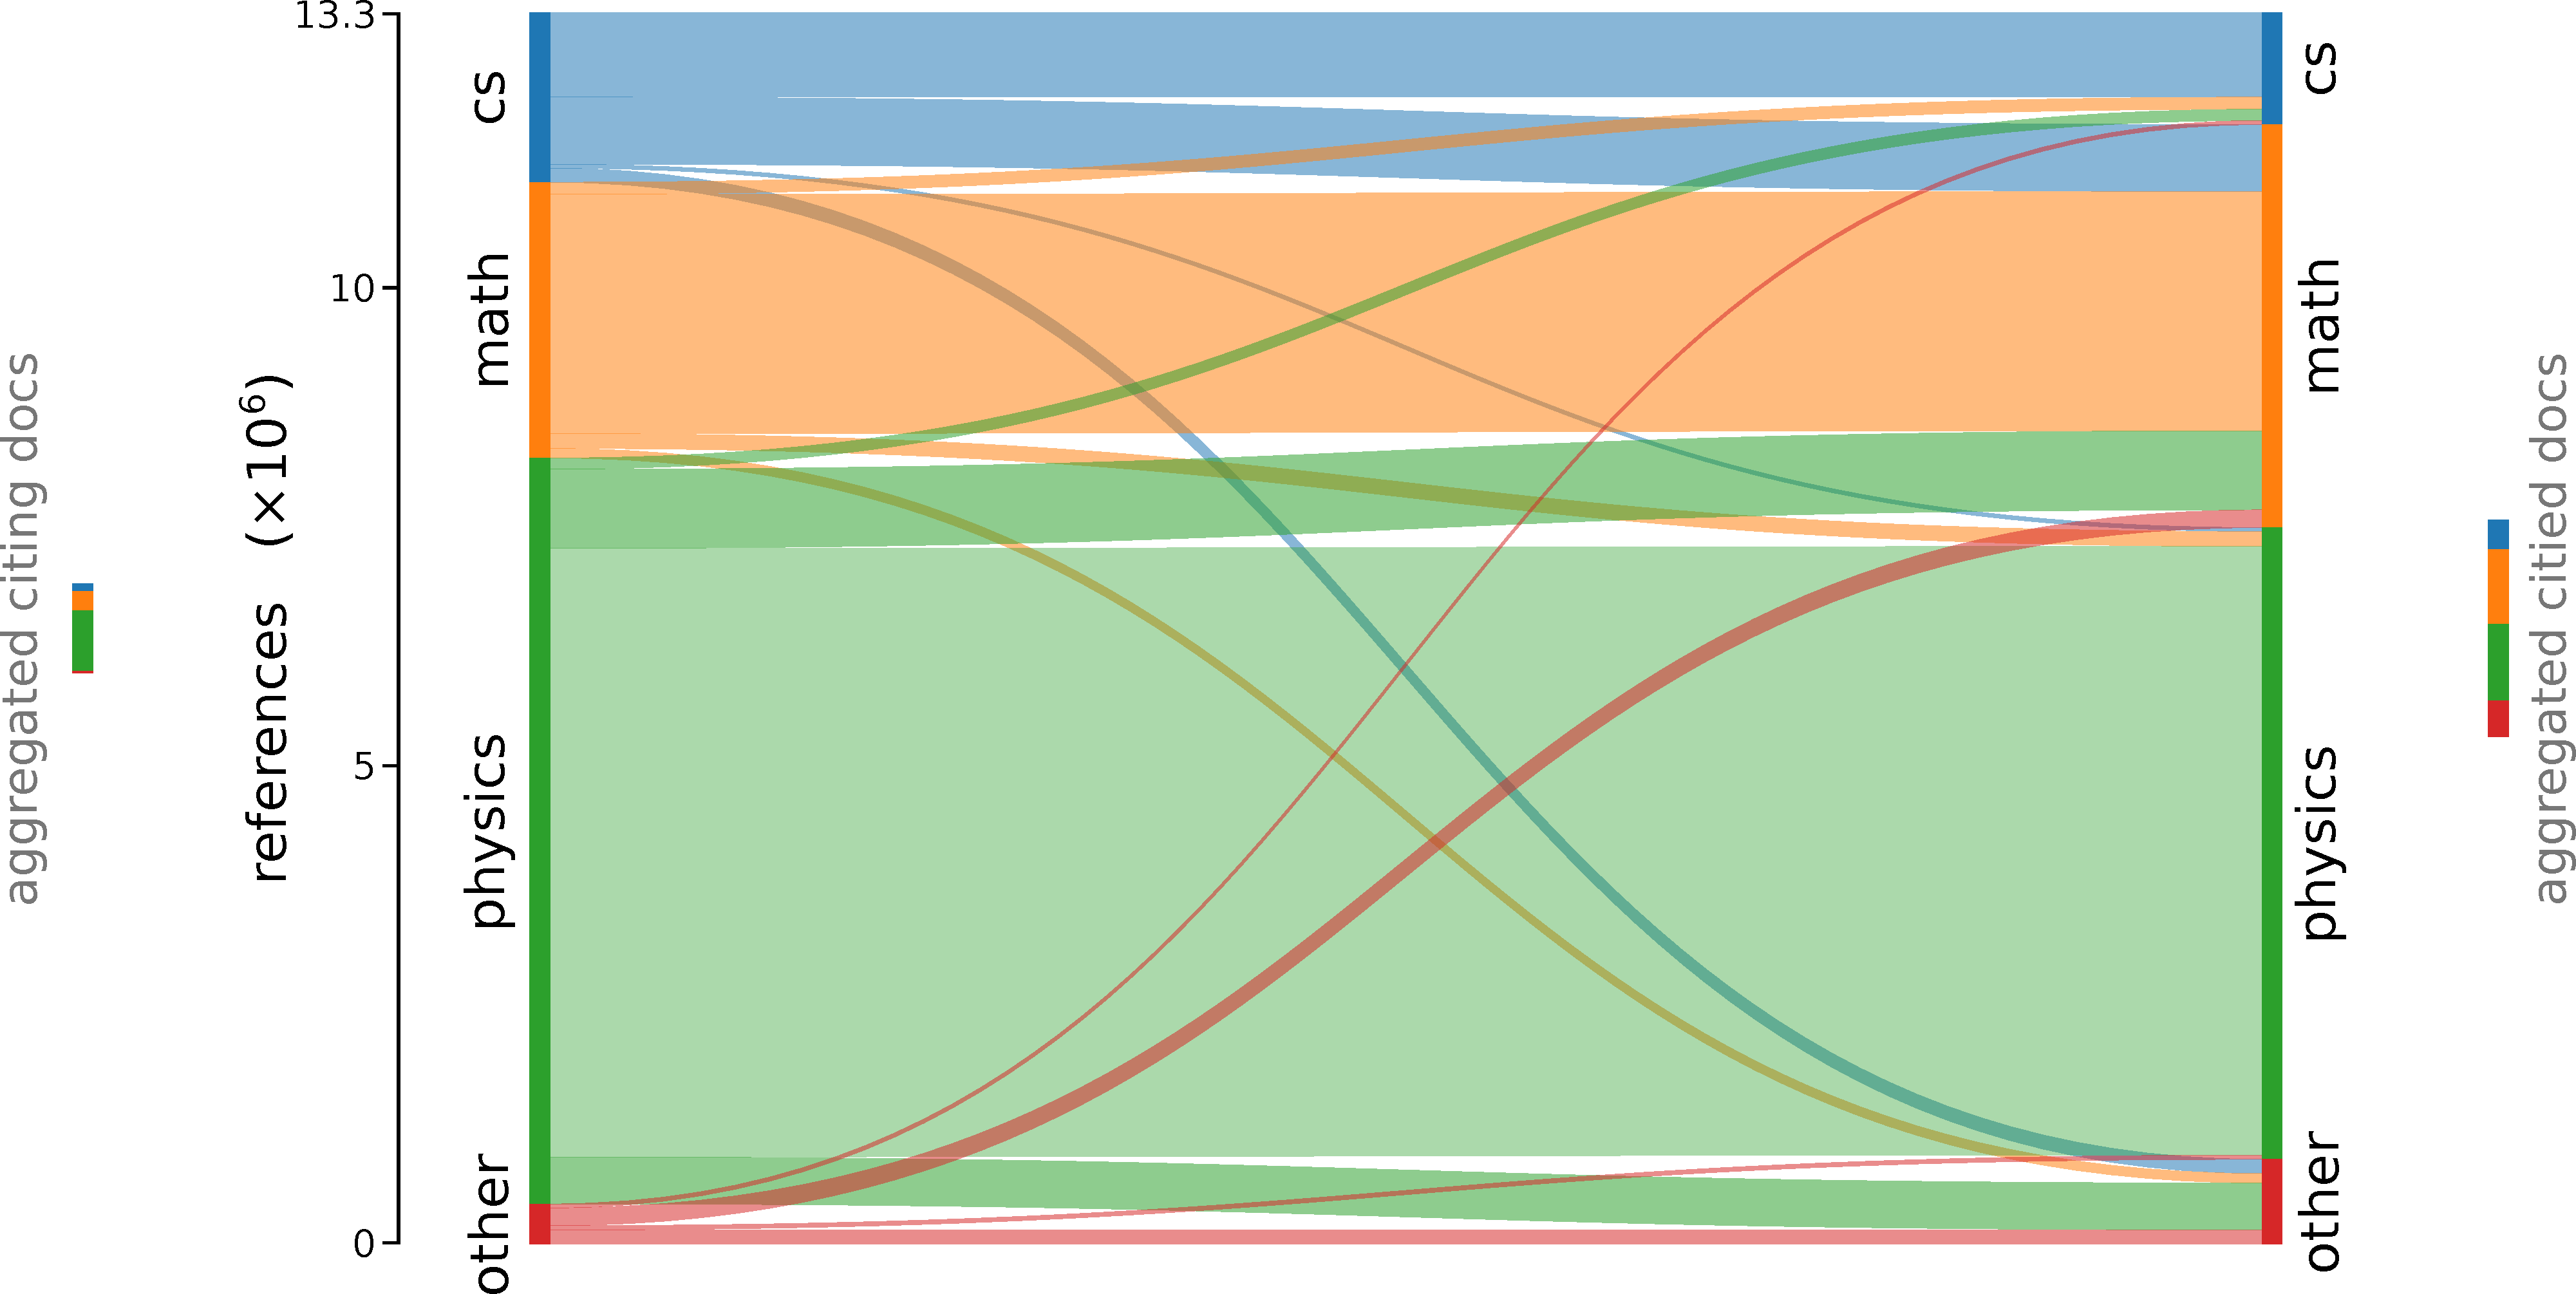
\includegraphics[width=\textwidth]{figures/dataset/citation_relation_sankey.pdf}
  \caption[Citation flow by field of study for 13.3 million reference items.]{Citation flow by field of study for 13.3 million reference items. For reference, the number of citing and cited documents per field of study are plotted on the sides.}
  \label{fig:sankey}
\end{figure}

By generating our data set from \LaTeX{} sources we were able to ensure clean text output as well as accurate citation information and exact citation marker positions. In terms of size it is closer to CiteSeerX and PMC-OAS than the smaller data sets available. The fact that the data set spans multiple disciplines also allows for comparisons in citing behaviour between these disciplices. Because references are already resolved to MAG IDs, the data set is readily usable for recommendation tasks and allows for the use of rich metadata on both the citing and cited document side. Lastly, the embedding of citation markers in the full plain text of papers instead of pre-extraction enables users of the data set to choose and compare citation context lenghts and variations at will.

    \chapter{Approach}\label{chap:approach}
In order to investigate the use of explicit semantic representations for the task of local citation recommendation we first need to decide which kinds of semantic constructs we want to model. As a starting point for this we looked into the field of citation context analysis~\cite{HERNANDEZ-ALVAREZ2016}. A common task in this area is the classification of citation contexts by their polarity (positive/neutral/negative) and function (often based on the four dimensions identified by Moravcsik et al.~\cite{Moravcsik1975}, conceptual/operational, evolutionary/juxtapositional, organic/perfunctory, conformative/negational). Such approaches are primarily concerned with the \emph{intent} of the author rather than the \emph{content} of what is being cited. We can therefore not expect to derive types of semantic constructs directly from citation functions. Starting from an established typology of citation functions will, however, ensure that we consider a wide range of different citations rather than cherry picking those that fit our preconceptions.

\begin{table}[]
\centering
    \caption{Semantic constructs in citation contexts from a range of citation functions used in the field of citation context analysis.}
    \label{tab:citfunctions}
\begin{center}
    \begin{tabular}{m{2.7cm}lm{8.5cm}}
    \toprule
    Function & Construct & Examples (semantic construct \emph{highlighted})\\
    \midrule
    Attribution & claim & ``Berners-Lee et al.~\cite{Berners-Lee2001} argue that \emph{structured collections of information and sets of inference rules are prerequesites for the semantic web to function}.'' \\\noalign{\smallskip}
    \  & NE & ``A variation of this task is `\emph{context-based co-citation recommendation}'~\cite{Kobayashi2018}.'' \\\noalign{\smallskip}
    \  & - & ``In \cite{Duma2014} Duma et al. test the effectiveness of using a variety of document internal and external text inputs to a TF-IDF model.'' \\\noalign{\medskip}
    Exemplification & NE & ``We looked into approaches to \emph{local citation recommendation} such as~\cite{He2010,Huang2014,Huang2015,Duma2014,Duma2016,Ebesu2017,Kobayashi2018,Jeong2019} for our investigation.'' \\\noalign{\medskip}
    Further reference & - & ``See \cite{Niklaus2018} for a comprehensive overview.'' \\\noalign{\medskip}
    Statement of use & NE & ``We use \emph{CiteSeerX}~\cite{Caragea2014} for our evaluation.'' \\\noalign{\medskip}
    Application & NE & ``Using this mechanism we perform `\emph{context-based co-citation recommendation}'~\cite{Kobayashi2018}.'' \\\noalign{\medskip}
    Evaluation & - & ``The use of DBLP in \cite{Faerber2018} restricts their data set to the field of computer science.'' \\\noalign{\medskip}
    Establishing links between sources& claim & ``A common motivation brought forward for research on citation recommendation is that \emph{finding proper citations is a time consuming task} \cite{He2010,He2011,Ebesu2017,Kobayashi2018}.'' \\\noalign{\smallskip}
    \  & - & ``Lamers et al.~\cite{Lamers2018} base their definition on the author's name whereas Thompson~\cite{Thompson2001} focusses on the grammatical role of the citation marker.'' \\\noalign{\medskip}
    Comparison of own work with sources& claim & ``Like \cite{Faerber2018} we find that, albeit written in a structured language, \emph{parsing \LaTeX{} sources is a non trivial task}.'' \\
    \bottomrule
    \end{tabular}
\end{center}
\end{table}

Table~\ref{tab:citfunctions} lists categories of citation functions along with the kinds of semantic constructs that can be found in such citation contexts. The list of citation functions is taken from \cite{Petric2007} (and therein built upon \cite{Thompson2001}). This study was selected because it gives an overview of previous attempts to classify citations, presents their new typology with extensive explanation as well as example contexts, and does not mix polarity into its function categories. Examining contexts from each of the eight functions we identify two types of semantic constructs: named entities (NE) and claims (or statements). The rationale behind these two is as follows. Named entities can identify reference publications for a certain data set/tool/concept (see \emph{Attribution}, \emph{Statement of use} and \emph{Application} in Table~\ref{tab:citfunctions}) as well as a method/field of study common to a selection of publications (see \emph{Exemplification} in Table~\ref{tab:citfunctions}). Claims can identify publications that can be cited to back or support the very claim contained in a citation context. Note that the example contexts listed to have no construct (``-'' in the \emph{Construct} column) may contain named entities and claims as well (e.g. ``DBLP'' or ``Lamers et al. base their definition of the author's name''), but these are (in the case of NEs) not representative of the cited work or (in the case of claims) just statements \emph{about} a publication rather than statements being backed by the cited work.
A third semantic construct that can be considered, but would require considering a larger citation context, is argumentative structures. To keep the scope of this thesis at a reasonable level we will, however, limit our investigation to named entities and claims.

The following sections will describe our investigation of entity based and claim based models for local citation recommendation.

\section{Entity based recommendation}
The intuition behind an entity based approach is, that there exists a reference publication for a named entity. Examples would be a data set (``CiteSeerX~\cite{Caragea2014}''), a tool (``Neural ParsCit~\cite{Animesh2018}'') or a concept (``Semantic Web~\cite{Berners-Lee2001}''). In a more loose sense this can also include publications being referred to as examples (``approaches to local citation recommendation~\cite{He2010,Huang2014,Huang2015,Duma2014,Duma2016,Ebesu2017,Kobayashi2018,Jeong2019}'').
% mention DBpedia Spotlight tests? (sufficient data available?)
For the identification of such named entities we take two approaches. A more strict one based on the fields of study given in the MAG, and a more loose one based on noun phrases.

\subsection{Fields of study in the MAG}
Along with papers, authors, venues etc. the MAG data schema also includes fields of study (FoS) that are associated with papers and interlinked in a child-parent manner. At the time of writing there are 229,716 FoS at 6 levels of granularity. They range from the most coarse level 0 (example entries being \emph{mathematics}, \emph{sociology},  \emph{computer science}) to more and more fine grained entities (\emph{information retrieval}$_{(1)}$→\emph{search engine}$_{(2)}$→\emph{web search query}$_{(3)}$→\emph{ranking (information retrieval)}$_{(4)}$→\emph{Okapi BM25}$_{(5)}$). The levels of granularity don't seem to follow a globally consistent pattern though. \emph{WordNet}, for example, being a particular piece of data in the same way \emph{Okapi BM25} is a particular function, is not at level 5 but level 2 (\emph{computer science}$_{(0)}$→\emph{artificial intelligence}$_{(1)}$→\emph{WordNet}$_{(2)}$). Another noteworthy aspect is that a FoS can have multiple parents (\emph{search engine} for example has a second parent in \emph{World Wide Web}).

\paragraph{Model} The entity based representation of a citation context is the set of FoS that appear within the context. Formally, let $\mathcal{F}$ denote the set of FoS; then the entity based representation of a citation context $c$ is the set of terms $t$ defined as ${R_{\text{FoS}}(c) = \{t|t\text{ appears in }c \land t\in \mathcal{F}\}}$. Because of the hierarchical structure of FoS we experiment with augmenting the set by including the set members' parents into the representation. We find that his leads to worse results, presumably because a context's description becomes more vague which is detrimental to identifying reference publications or exemplifications. We furthermore look into only using a FoS when it directly precedes the citation marker---as it might be more relevant to the citation then---, but notice that such cases are too rare. In a preliminary test with 900k citation contexts, only 0.14\% of our 180k test set items have a FoS in the required position matching any of the representations learned from the training set.

\paragraph{Recommendation} For recommending documents based on $R_{\text{FoS}}$ we use the Jaccard similarity between the input citation context and the aggregrated citation contexts describing each candidate document. Formally, let $c_i$ denote the input citation context and $\mathcal{D}$ be a set of documents with members $d\in \mathcal{D}$. Furthermore let $\varrho(d)$ be the set of citation contexts referencing $d$; ${\varrho(d)=\{c|c\text{ references } d\}}$. The Jaccard similarity then is defined as ${J(A,B)=\frac{|A\cap B|}{|A\cup B|}}$, where $A = R_{\text{FoS}}(c_i)$ and $B=\bigcup\limits_{c \in \varrho(d)} R_{\text{FoS}}(c)$.

\subsection{Noun phrases}
For our second entity based model we take a more loose approach and treat noun phrases extracted from the arXiv data set as named entities. By filtering out items that appear only once we end up with 2,835,929 noun phrases (NPs).

\paragraph{Model} Similar to the FoS representation, we look at the NPs appearing within a citation context. To ensure a high descriptiveness, we only take into account maximally long matches. A context \emph{``This has been done for language model training [27]''}, for example, would have ``language model training'' in its representation, but not ``language model''. Formally we can define ${R_{\text{NP}}(c) = \{t|t\text{ appears in }c \land t\in \mathcal{P} \land t^{+pre} \notin \mathcal{P}\land t^{+suc} \notin \mathcal{P}\}}$ where $\mathcal{P}$ is our set of NPs while $t^{+pre}$ and $t^{+suc}$ denote an extension of $t$ using its preceding or succeeding word respectively. As an alternative representation we furthermore define ${R_{\text{NPmrk}}^{2+}(c)}$ as a subset of ${R_{\text{NP}}(c)}$ containing, if present, the NP of minimum word length 2 directly preceding the citation marker in $c$ that a prediction is to be made for. Formally, ${R_{\text{NPmrk}}^{2+}(c) = \{t|t\in R_{\text{NP}}(c)\land len(t)\geq 2 \land t\text{ directly precedes } m\}}$ where $m$ is the citation marker in $c$ that a prediction is to be made for.

\paragraph{Recommendation} Recommending documents based on ${R_{\text{NP}}}$ and ${R_{\text{NPmrk}}^{2+}}$ is done using a vector space model (VSM) in which NP representations, treated as a bag of word (BoW), are compared by their cosine similarities. Representations of candidate documents are, likewise to the FoS based model, aggregrates over all contexts referencing the document. Formally, the vector representation of a context is given by $V(R(c)) = (t_{1,j}, t_{2,j}, ..., t_{|\mathcal{P}|,j})$ where $\mathcal{P}$ is the set of all NPs % technically wrong b/c sets are not ordered
and $t_{i,j}$ is a non-negative integer representing a quantity with regards to the $i$th term in $\mathcal{P}$. Aggregated context representations for candidate documents are caluclated by adding up all vector representations of the contexts referring to a document. I.e., let $\varrho(d)$ be the set of citation contexts referencing $d$, then $d$'s vector representation is $\sum\limits_{c \in \varrho(d)} V(R(c))$. The similarity between an input context $c_i$ and a candidate document $d\in \mathcal{D}$ can then be calculated as the cosine $\theta$ between the two vector representations ${\mathrm{cos}(\theta)=\frac{A\cdot B}{\|A\| \|B\|}}$ where  $A=V(R(c_i))$ and $B=\sum\limits_{c \in \varrho(d)} V(R(c))$.

\section{Claim based recommendation}
%For the introduction of a claim based model we first need to make a few observations on how citations interact with the text they're placed in. By convention, citations are constructed by placing a type of marker, which identifies an entry in the document's reference section, in the text. These markers can, depending on discipline, journal, etc. take different forms. Some examples are numbers in square brackets (``In [27] ...''), alphanumeric identifiers in square brackets (``In [Bol98] ...''), a year in parentheses succeeding an author's name (``Swales (1990) has argued ...'') and an author's name with a year in parentheses (``It has been argued (Swales, 1990) ...''). Named entities can stand in a grammatical relation to such a marker. In ``By using CiteSeer, [Bol98], we ...'', for example, the named entitiy \emph{CiteSeer} and the citation marker \emph{[Bol98]} are in a grammatical relation called \emph{apposition}. A citation marker can, however, reasonably assumend to never be \emph{part of} the named entity. This is different in the case of the statements within a citaiton context. Looking at the sentence ``In \cite{Bollacker1998} Bollacker et al. introduce Citeseer.'' we can see that the marker itself is part of what is being said, while this is not the case in, for example, ``Bollacker et al. introduced Citeseer in 1998~\cite{Bollacker1998}.''. Citations w
For the introduction of a claim based model we first need to make a few observations on how citations interact with the text they're placed in. Citing is done by placing a citaiton marker (that has a corresponding entry in the reference section) in the text. Such a marker is sometimes put into a sentence such that it functions as a word (e.g. ``In \cite{Bollacker1998} Bollacker et al. introduce Citeseer.'' or ``For further details see \cite{Bollacker1998}.'') and sometimes detached from the sentence's grammatical structure (e.g. ``Bollacker et al. introduced Citeseer in 1998~\cite{Bollacker1998}.'' or ``CiteSeer~\cite{Bollacker1998} was introduced in 1998.''). Put differently, in the latter two examples the sentences work just fine without the citation markers (``Bollacker et al. introduced Citeseer in 1998.'', ``CiteSeer was introduced in 1998.'') while the former two become ungrammatical or change in meaning (``In Bollacker et al. introduce Citeseer.'', ``For further details see.''). As suggested in \cite{Whidby2011} and \cite{Abujbara2012}, we will refer to citations where the citation marker has a grammatical function as ``syntactical'', and to ones where the citation marker is not part of the actual setence as ``non-syntactical''  (a more detailed discussion of this and related terminology can befound in Appendix~\ref{chap:integralsyntactic}). This distiction will be relevant because claims within a citation context can, in the case of syntactical citations, be in a grammatical relation to or even contain citation markers.

The following sections will describe our evaluation of tools for extracting claims from citation contexts and the model we developed for recommendation.

\subsection{Tools for extracting claims}
For the extraction of claims we consider a total of four state of the art \cite{Zhang2017} information extraction tools: PredPatt~\cite{White2016}, Open IE 5.0~\cite{Mausam2016}, ClausIE~\cite{DelCorro2013} and Ollie~\cite{Mausam2012}. All of these can identify information in unformatted text, which they output in some form of predicate-argument tuples. Listing~\ref{lst:ietools} shows the output of all four tools for the simple sentence \emph{``The paper shows that context-based methods can outperform global approaches.''}.

\begin{lstlisting}[caption={Information extraction tool output examples.},label={lst:ietools}]
# PredPatt
?a shows ?b
    ?a: The paper
    ?b: SOMETHING := context-based methods can outperform global approaches
?a can outperform ?b
    ?a: context-based methods
    ?b: global approaches

# Open IE 5.0
0.90 Context(The paper shows,List([0, 15))):(context-based methods; can outperform; global approaches)
0.78 (The paper; shows; that context-based methods can outperform global approaches)

# ClausIE
"The paper" "shows" "that context-based methods can outperform global approaches"
"context-based methods" "can outperform" "global approaches"

# OLLIE
0.659: (context-based methods; can outperform; global approaches)[attrib=The paper shows]
\end{lstlisting}

Because the output for simple sentences is comarable for all of the tools, we tested them on 5 non trivial citation contexts, each consisting of 3 sentences. Based on this evaluation---the details of which are given in Appendix~\ref{chap:claimextooleval}---we deem PredPatt to perform the best, which is consistent with the observations in \cite{Zhang2017}.

% also: Survey on open information extraction\cite{Niklaus2018}

% context specific claim detection\cite{Levy2014}

% if only papers where semantically annotated as proposed in \cite{BuckinghamShum2000}
\subsection{A predicate-argument model}
Starting out with the predicate-argument tuples as PredPatt outputs them, we tested if there was enough of an overlap betweeen the components among citation contexts to facilitate recommendation. Taking the example from Listing~\ref{lst:ietools}, we would note the predicates \emph{``show''} and \emph{``can outperform''} as well as the arguments \emph{``The paper''}, \emph{``context-based methods can outperform global approaches''}, \emph{``context-based methods''} and \emph{``global approaches''}. Even when not preserving the associations between predicates and their arguments---e.g. looking for other contexts where \emph{``global approaches''} was identified without requiring it to be in conjunction with \emph{``can outperform''}---, we note very little overlap between citation contexts. We believe this to be the case because the predicates and especially arguments that PredPatt identifies can get very long, like \emph{``can outperform''} (including the auxilliary verb \emph{``can''}) and \emph{``context-based methods can outperform global approaches''} (unlikely to appear in another citation context with the exact same wording).

\begin{figure}
  \centering
    \subfloat[Main clause.]{{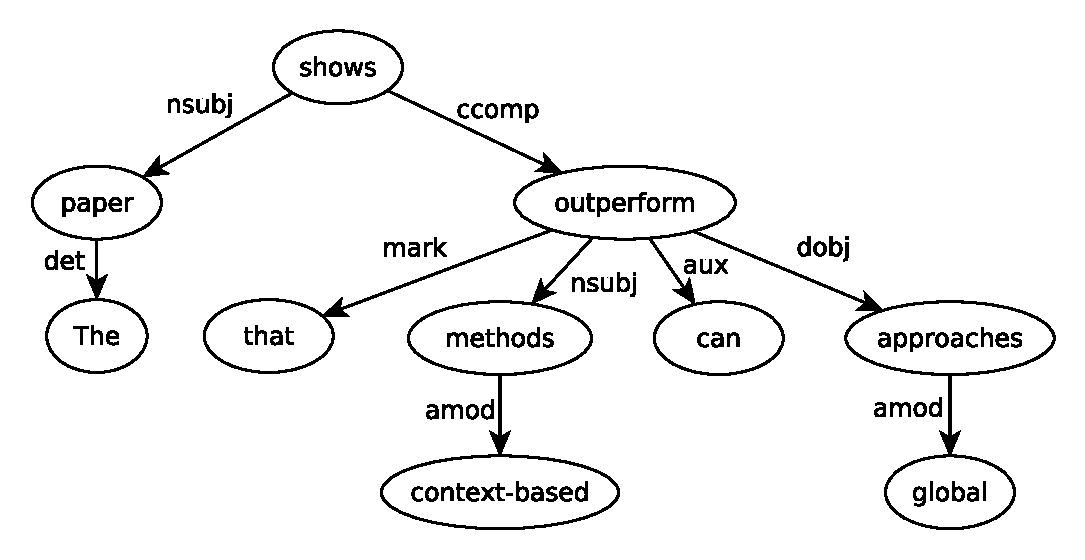
\includegraphics[width=.55\textwidth]{figures/approach/pp_tree0.pdf}}\label{fig:pptrees0}}
    \subfloat[Sub clause.]{{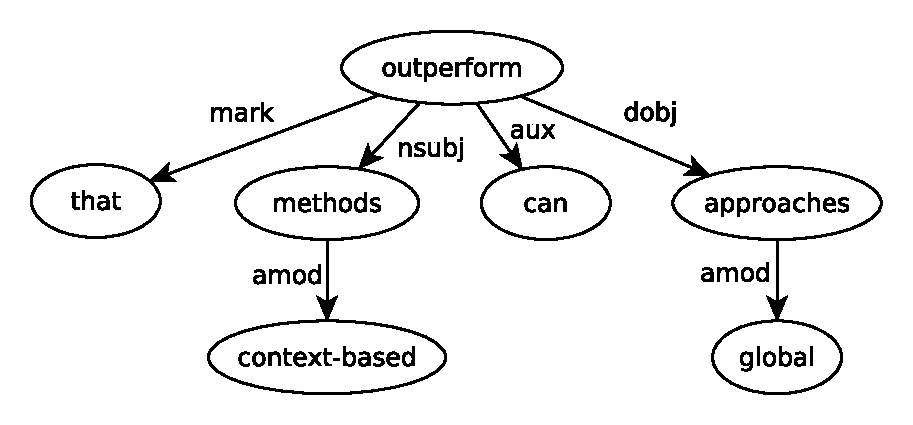
\includegraphics[width=.45\textwidth]{figures/approach/pp_tree1.pdf}}\label{fig:pptrees1}}
  \caption{UD trees as generated by PredPatt.}
  \label{fig:pptrees}
\end{figure}

To overcome this problem we develop a derivate model based on PredPatt's internal representation of sentences. Internally, PredPatt represents sentences in a tree structure based on Universal Dependencies (UD)~\cite{Nivre2016} (i.e. a dependency grammar as opposed to a constituency grammar). This means words are connected by directed edges where the source is referred to as \emph{governor}, the target is referred to as \emph{dependant} and the edge itself is associated with a type of \emph{relation}. Looking at Figure~\ref{fig:pptrees}, depicting PredPatt's internal view on the example sentence given in Listing~\ref{lst:ietools}, we can, for example, see that the \emph{``can''} is a dependant to and governed by \emph{``outperform''} in an auxilliary relation. How our (predicate-argument based) claim model is constructed from this tree structure and used for recommendation will be discussed in the following sections.

\begin{algorithm}
\caption{Construction of $R_{\text{claim}}(c)$}
\label{alg:pprep}
\begin{algorithmic}
    \State $c \gets \mathit{strip\_quotation\_marks}(c)$     \alignedComment{remove quotation marks}
    \State $c \gets \mathit{merge\_citation\_markers}(c)$     \alignedComment{e.g. ``CIT , CIT''→``CIT''}
    \State $\mathit{pp\_trees}_c \gets \mathit{predpatt}(c)$     \alignedComment{get PredPatt output}
    \State $\mathit{output} \gets []$     %\alignedComment{empty array}
    \State $\mathit{resolve\_rels} \gets [\text{'name'},\text{'goeswith'},\text{'mwe'},$     \alignedComment{\textbf{(b$_\mathbf{1}$)} UD relations}
    \State $\hphantom{\mathit{resolve\_rels} \gets [}\text{'compound'},\text{'conj'},\text{'amod'},$
    \State $\hphantom{\mathit{resolve\_rels} \gets [}\text{'advmod'}]$
    \ForEach{$t\in\mathit{pp\_trees}_c$}   \alignedComment{for all claims identified}
        \State $\mathit{root} \gets \mathit{get\_root}(t)$   %\alignedComment{get predicate}
        \State $\mathit{pred} \gets \mathit{identify\_predicate}(t)$   \alignedComment{\textbf{(a)} resolve copula if present}
        \State $\mathit{pred} \gets \mathit{lemmatize}(\mathit{pred})$   %\alignedComment{lemmatize}
        \ForEach{$n\in\mathit{traverse}(t)$}    %\alignedComment{traverse all nodes}
            \If{$\mathit{pos\_tag}(n) == \text{'NOUN'}$}   %\alignedComment{if it's a noun}
                \State $\mathit{arg} \gets \mathit{resolve\_all}(n, \mathit{resolve\_rels})$   \alignedComment{\textbf{(b$_\mathbf{2}$)} resolve compounds etc.}
                \State $\mathit{output.append}(\mathit{pred}+\text{':'}+\mathit{arg})$   \alignedComment{build pred:arg tuple}
            \EndIf
        \EndFor
    \EndFor\\
    \Return{$\mathit{output}$}
\end{algorithmic}
\end{algorithm}

\paragraph{Model} The construction of our claim representation $R_{\text{claim}}(c)$ for a citation context $c$ is shown in Algorithm~\ref{alg:pprep}. There are two preprocessing steps prior to applying PredPatt. Quotation marks matching the regular expression \texttt{[“”„"«»‹›$\mathtt{\langle\hspace{-1mm}\langle\rangle\hspace{-1mm}\rangle\langle\rangle}$]} are removed to avoid parsing errors, and groups of citation marker replacement tokens (e.g. \emph{``CIT , CIT , CIT''} originating from e.g. \emph{``[3,27,42]''}) are merged into one (i.e. \emph{``CIT''}) to get a cleaner and easier to parse sentence structure. After applying PredPatt, the UD tree of each of the identified claims is traversed and predicate-argument tuples are generated. A claim is always centered around a predicate, which is the root of the corresponding UD tree unless a compula (\emph{be}, \emph{am}, \emph{is}, \emph{are}, \emph{was}) is used, in which case the predicate is a dependant of the root node with the relation type \emph{``cop''} (this is handled at marker \textbf{(a)} in Algorithm~\ref{alg:pprep}). Once identified, predicates are lemmatized using NLTKs WordNetLemmatizer. For the identification of useful arguments (markers \textbf{(b$_\mathbf{1}$)} and \textbf{(b$_\mathbf{2}$)} in Algorithm~\ref{alg:pprep}), we look at all nouns within the UD tree and resolve compounds (\emph{``compound''}, \emph{``mwe''}, \emph{``name''} relations), phrases split by formatting (\emph{``goeswith''}), conjunctions (\emph{``conj''}) as well as adjectival and adverbial motifiers (\emph{``amod''}, \emph{``advmod''}). To give an example, the noun \emph{``methods''} in both trees in Figure~\ref{fig:pptrees} has the adjectival modifier \emph{``context-based''}. In such a case our model would not choose \emph{``methods''} as an argument to \emph{``outperform''} but \emph{``context-based methods''}. Listing~\ref{lst:ppmodel} shows the complete representation generated for the example sentence.

\begin{lstlisting}[caption={An example of $R_{\text{claim}}(c)$.},label={lst:ppmodel}]
[
 'show:paper',
 'show:context based methods',
 'show:global approaches',
 'outperform:context based methods'
 'outperform:global approaches',
]
\end{lstlisting}

As becomes apparent when looking at Listing~\ref{lst:ppmodel}, we do not preserve the order of arguments. I.e., instead of constructing a triple (e.g. \texttt{context based methods:outperform:global approaches}) we build two tuples (\texttt{outperform:context based methods} and \texttt{outper\-form:global approaches}). This sequential invariance means a certain loss in precision, but also allows us to capture the similarity between active voice and passive voice sentences without the need to ensure reliabe parsing of such grammatical constructs. The input \emph{``The paper shows that global approaches can be outperformed by context-based methods.''}, for example, also has the claim representation shown in Listing~\ref{lst:ppmodel}.

\paragraph{Recommendation} To make use of $R_{\text{claim}}$ for recommendation we use a VSM where each dimension is a predicate-argument tuple. Similarities within this VSM are calculated as cosines between TFIDF-weighted vectors. Formally, the vector representation of a context is given by $V(R(c)) = (t_{1,j}, t_{2,j}, ..., t_{|\mathcal{T}|,j})$ where $\mathcal{T}$ is the set of all predicate-argument tuples % technically wrong b/c sets are not ordered
and $t_{i,j}$ is a non-negative integer representing a quantity with regards to the $i$th tuple in $\mathcal{P}$. TFIDF values for each $t_{i,j}$ in $V(R(c))$ with respect to a collection of contexts $\mathcal{C}$ are calculated as $\mathit{TFIDF}(t, c, \mathcal{C}) = \mathit{tf}_{t,c} \times \mathit{idf}_{t,\mathcal{C}}$, where $\mathit{tf}_{t,c}$ denotes the number of occurences of $t$ in $c$, and $\mathit{idf}_{t,\mathcal{C}} = \mathit{log}\frac{|\mathcal{C}|}{|\{c\in\mathcal{C}|t\text{ appears in }c\}|}$ is the log of the number of contexts over the number of contexts containing $t$.

Likewise to ${R_{\text{NP}}}$, aggregated context representations for candidate documents are caluclated by adding up all vector representations of the contexts referring to a document. Again, let $\varrho(d)$ be the set of citation contexts referencing $d$, then $d$'s vector representation is $\sum\limits_{c \in \varrho(d)} V(R(c))$. The similarity between an input context $c_i$ and a candidate document $d\in \mathcal{D}$ can then be calculated as the cosine $\theta$ between the two vector representations ${\mathrm{cos}(\theta)=\frac{A\cdot B}{\|A\| \|B\|}}$ where  $A=\mathit{TFIDF}(V(R(c_i)))$ and $B=\mathit{TFIDF}\Big(\sum\limits_{c \in \varrho(d)} V(R(c))\Big)$.

% As a variation, we also define a model that combines $R_{\text{claim}}$ similarities with BoW similarities.

% predicates could be grouped/clustered to represent functions as in \cite{Gabor2018}

% alternative view: model gives a selective citation context derived from claim structure (cf. concept of reference scope as sub part of citation context sentence\cite{Abujbara2012,RAHUL2017}

    \chapter{Evaluation}\label{chap:evaluation}
To measure the effectiveness of our models we evaluate them in offline and online settings. The details of these can be found in Section~\ref{sec:offeval} and \ref{sec:oneval} respectively. Before that, we will discuss the peculiarities of evaluating approaches to citation recommendation in Section~\ref{sec:citrecspecial}.

\section{Special considerations for citation recommendation}\label{sec:citrecspecial}
The goal in many recommendation domains is to identify items a user is likely to engage with, like finding products a user might buy or media a user might want to consume. The relevance judgement of a recommended item in such a case is merely based on the user's subjective taste.
% In other words, if the reciever of a recommendation is satisfied with it, there is no ground for arguing that the recommendation was wrong.
With citations there is more to it than just preference. For a recommended citation to be useful to a researcher it has to be appropriate. To give an example, if the video platform PeerTube recommends watching \emph{Paywall: The Business of Scholarship}, there is no ground for arguing this recommendation could never be valid. However, if a citation recommendation system suggests to cite \emph{Alan Turing, ``On Computable Numbers, with an Application to the Entscheidungsproblem'', 1937} in the context \emph{``We use CiteSeerX [] for our evaluation.''}, then this is arguably not usable. This circumstance makes the evaluation of approaches to citation recommendation comparably difficult, because the accurate judgement of relevance (and by extension applicability) of a recommended item for a given input requires expert knowledge. This has to be kept in mind when automatically generating ground truths for offline evaluations and also when interpreting evaluation results.

% Their purpose is not to please their author, but to relate new scholarly work to existing one by means of attribution, backing, critique etc. As a tool in the rather rigid realm of scientific discourse, they have to abide by established conventions and reflect reality. While a movie recommendation cannot be wrong, a citation recommendation easily can.

% A common method for evaluating recommender systems is to use items that have existing relevance judgements (e.g. movies with user ratings logged on a website) as an input to the system and compare the output with the actual user judgement. A similar practice exists in citation recommendation. Citation contexts from existing publications are stripped of their citations, fed into the recommender and the result is compared to the original citation. 

A common source of ground truths for automatically evaluating recommender systems is existing relevance judgements (e.g. movies with user ratings logged on a website). For evaluation these are used as an input to the system and the output is compared with the actual judgement. The equivalent in citation recommendation is to harvest citation contexts from existing publications and trying to re-predict the citaions originally contained. While in the case of a movie recommendation, the user's rating at the point in time it was made is \emph{the} truth---within the bounds of the user's introspective capabilities---, a citation, albeit in a published work, can be flawed or may be one of several possibly valid ones. Awareness of this is helpful for interpreting evaluation results in re-prediction scenarios and also the motivation behind alternative evaluation metrics. % (see also Section~\ref{sec:offeval})

Another aspect of automatically harvested ground truth is change over time. In our movie recommendation example this can manifest in a user's taste changing. In scholarly discourse, a cited documents role---that is, how or if it is cited---can develop over time~\cite{Swales1986,He2018}. Examples of causes are concepts becoming obsolete through new discoveries (e.g. the expanding Earth~\cite{Wu2011}), discoveries becoming named retrospecively (e.g. Lotka's law~\cite{Potter1981}) and important work within a field becoming established knowledge and not being referred to anymore (e.g. physicists not citing Einstein's 1905 paper \emph{``Zur Elektrodynamik bewegter Körper''} when talking about the theory of relativity). This observation motivates harvesting citation contexts for ground truths preferably from recent publications which can be achieved through a temporal split of training and test data. % (see also Section~\ref{sec:offeval})

A last important consideration has to be made concerning the split of training and test data. A na\"{\i}ve way of doing this would be to group citation contexts by cited document and then split each group into, for example, 80\% training and 20\% test data. This would ensure all cited documents are tested for. However, it would also lead to cases where citation contexts from a single publication are split. This would mean an author's word choice, writing style, etc. could be an unwanted signal informing the recommendation. Fortunately, a temporal split of training and test data as mentioned in above paragraph (i.e. splitting training and test data by pulication date of citing documents) automatically solves this problem.

% FIXME: temporal split also ensures that contexts are split document wise, which is important, b/c splitting on a context and not document level can lead to an authors writing style etc. being a signal (TODO write this properly)

% Lastly, the number of contexts describing a recommendation item, ...

% candidates are only citations within current paper\cite{Duma2014}

\begin{table}[b]
\centering
    \caption{Key properties of data sets used for evaluation.}
    \label{tab:datasetprops}
\begin{center}
    \begin{tabular}{llrrrr}
    \toprule % CC/RC = citation contexts per recommendation candidate
    Data set & Train/test split & \#Cand. & \#Tested & \#Test set items & Mean CC/RC (SD)\\ 
    \midrule
    arXiv & $\le$2016 / $\ge$2017 & 63,239 & 49,980 & 490,018 & 21.7 (\hphantom{1}51.2) \\
    MAG & $\le$2017 / $\ge$2018 & 45,580 & 8,013 & 53,151 & 69.2 (137.3) \\
    RefSeer & $\le$2011 / $\ge$2012 & 184,539 & 17,323 & 53,401 & 18.2 (\hphantom{1}47.0)\\
    ACL-ARC & $\le$2005 / $=$2006 & 2,431 & 1,089 & 3,881 & \hphantom{1}6.8 (\hphantom{10}9.5) \\
    \bottomrule
    \end{tabular}
\end{center}
\end{table}

\section{Offline evaluation}\label{sec:offeval}
Our offline evaluation, in total, encompasses seven different models and four data sets. First, we will introduce the data sets used. We  employ citation contexts from arXiv, the MAG, RefSeer and ACL (see also Chapter~\ref{chap:dataset}).
Note that in all four cases we do not use all contexts available in the data set but rather apply filter criteria, the details of which can be found in Appendix~\ref{chap:offlineevalfilter}.
Table~\ref{tab:datasetprops} gives an overview of key properties of the resulting data. Given are the temporal split between train and test set, the number of candidates to rank (documents), number of these tested for (documents), the number of test set items (contexts) and the mean number of citation contexts trained on per recommendation candidate. This last measure is furthermore visualized in Figure~\ref{fig:evalcomp}. The amount of candidates to rank for each recommendation (\#Cand.) and how well these candidates are described (CC/RC) gives insight into how difficult the recommendation task for each of the data sets is. Comparing, for example, arXiv and MAG under the assumption the data is equally clean (which is not necessarily the case), recommendation using the MAG data should be the easier task, because there are fewer, better described candidates to rank. The number of cited documents tested for (\#Tested) and number of test set items (\#Test set items) are indicative of how comprehensive the evaluation is. Testing for 50k cited documents using 490k contexts (arXiv) can, for example, be considered more thorough than testing for 2.4k cited documents using 3.8k contexts (ACL-ARC).

% We perform an offline evaluation of several models on multiple data sets. Our main focus will be a subset of the arXiv data set described in Chapter~\ref{chap:dataset} and three of the models discussed in Chapter~\ref{chap:approach} plus a baseline. The arXiv subset is comprised of 1,835,797 citation contexts (7.5\% of the whole data set) generated by filtering with two conditions: the citing paper is from the field of computer science and the cited paper has at least five citing papers within the data set. The reasoning behind this is % comparability to online? annotation time? -> mby go with b/c time "to allow for also annotating other data sets"
% The contexts used from arXiv are filtered by two conditions: the citing paper is from the field of computer science and the cited paper has at least five citing papers within the data set. This results in 1,835,797 citation contexts (7.5\% of the whole data set). Our reason for this aggresive filtering is 

\begin{figure}[tb]
  \centering
    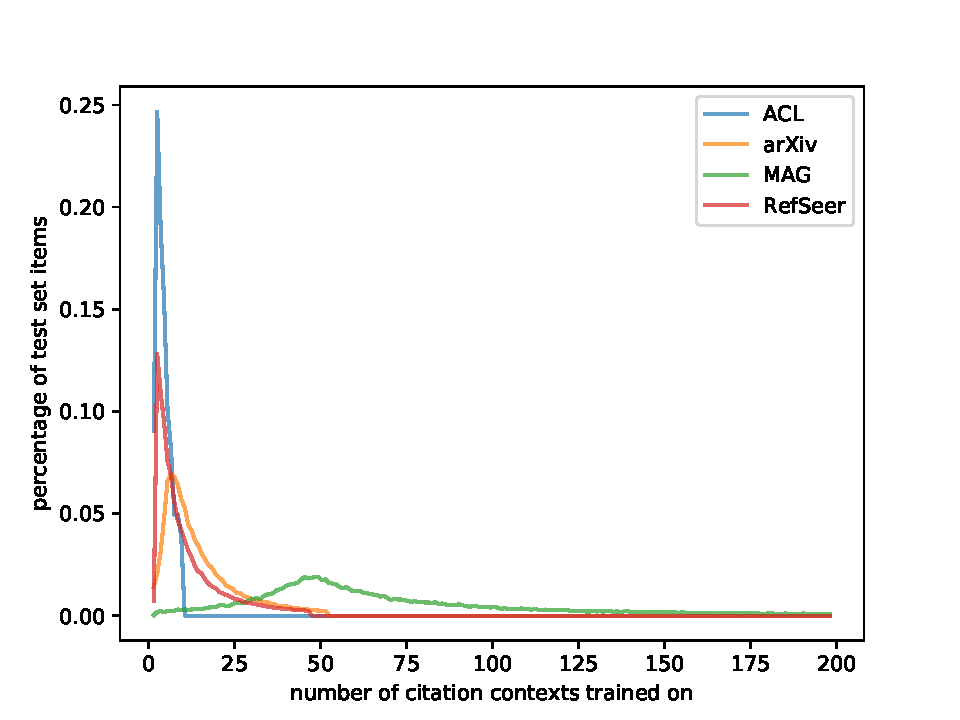
\includegraphics[width=.8\textwidth]{figures/evaluation/comparison_contexts_per_cited_doc.pdf}
  \caption{Number of citation contexts per recommendation candidate.}
  \label{fig:evalcomp}
\end{figure}

% In the following we will describe how the contexts were chosen from each of the data sets. In order to allow us to annotate\footnote{The calculation of NP and especially claim representations takes too much time to realisticly be done on the fly while learning and testing. These representations are therefore generated in a prior offline step.} and evaluate on several data sets with the available temporal and computational resources, we apply the following filter criteria to generate the data described in Table~\ref{tab:datasetprops}: arXiv contexts are those where the citing document is from the field of computer science and the cited document has at least 5 citing documents; MAG contexts are first filtered to be from the field of computer science, in English

The models used for recommendation are the four presented in Chapter~\ref{chap:approach}, ${R_{\text{FoS}}}$, ${R_{\text{NP}}}$, ${R_{\text{NPmrk}}^{2+}}$ and $R_{\text{claim}}$---which we will refer to as FoS, NP, NPmarker, and Claim from here on for simplicity---as well as a Bag-of-Words baseline (BoW) and two combined models (BoW+fosboost and Claim+BoW). The BoW baseline involves removal of punctuation as well as stopwords and uses TFIDF for ranking. We choose TFIDF over BM25 because the former shows better performance in our evaluations%
% \footnote{Maybe write a long footnote here about how BM25 gives comparable results to TFIDF when representations of cited documents are not jointly learned but contexts are treated separately, but this method in general gives worse results than using joinly learned representations}
. BoW+fosboost is constructed by taking the BoW ranking and then moving all candidates, where the overlap in fields of study (${\big|R_{\text{FoS}}(c_i)\cap\big(\bigcup\limits_{c \in \varrho(d)} R_{\text{FoS}}(c)\big)\big|}$, cf. Section~\ref{sec:approachfos}) is maximal, one position upwards in the ranking. Ranking in Claim+BoW is done by linearly combining similarity values $S(A,B)=\sum\limits_{m\in\mathcal{M}}\alpha_mS_m(A,B)$ of the models $\mathcal{M}=\{\text{Claim},\text{BoW}\}$ with heuristically determined coefficients $\alpha_{\text{Claim}}=1$ and $\alpha_{\text{BoW}}=2$.

Table~\ref{tab:arxivevalnumbers} shows NDCG, MAP, MRR and recall values at cut-off 5 for all models evaluated on the arXiv data. While FoS alone performs very poorly, the combined model BoW+fosboost consistently performs better then BoW alone. Nevertheless, because the performance gain is minute, we see no reason for a more detailed investigation of the models FoS and BoW+fosboost. Overall Claim+BoW shows the best performance, with NPmarker achieving the highest value for the MRR metric. To investigate the performance of these models further, we look at above metrics at different cut-off values and using multiple data sets. Note that arXiv is the only of our data sets where the NPmarker model is applicable (because the exact position of the citation marker is needed) and also the only of the data sets where more than one cited document in can be counted as relevant (cf. ``adjacent citations'' in Section~\ref{sec:datasetformat}).

% pre-filtering experiments (knn\cite{Bhagavatula2018}, lsi, lda, fos, ...)
% different evaluation settings (all, CSonly, comparison to MAG, ACL (data from \cite{Faerber2018b})...)
% FoS alone, restrictively combined w/ BOW, only directly preceeding, ...
% PP model alone, combined, ...

% -> not \emph{generally} applicable/beneficial but for certain citation types ...

% also mention \cite{Kobayashi2018} here b/c they specifically target cases where more than one citation is applicable (could be interpreted as either \emph{multiple (simultaneously)} for one context or \emph{several options that are all valid by themselves but in the end a single one is to be chosen} for one contexts)

\begin{table}[]
\centering
    \caption{Evaluation scores at cut-off 5 for all models using the arXiv data.}
    \label{tab:arxivevalnumbers}
\begin{center}
    \begin{tabular}{lllll}
    \toprule
    Model & NDCG@5 & MAP@5 & MRR@5 & Recall@5 \\
    \midrule
    Claim+BoW & \textbf{0.21829} & \textbf{0.34416} & 0.17530 & \textbf{0.27420} \\
    BoW+fosboost   & 0.20682 & 0.32980 & 0.16264 & 0.25824 \\
    BoW       & 0.20673 & 0.32961 & 0.16256 & 0.25817 \\
    NPmarker  & 0.17677 & 0.30769 & \textbf{0.17764} & 0.24931 \\
    Claim     & 0.08337 & 0.14441 & 0.07477 & 0.11750 \\
    NP        & 0.07914 & 0.13950 & 0.06775 & 0.10558 \\
    FoS       & 0.00921 & 0.01999 & 0.00420 & 0.00933 \\
    \bottomrule
    \end{tabular}
\end{center}
\end{table}

\begin{figure}
  \centering
    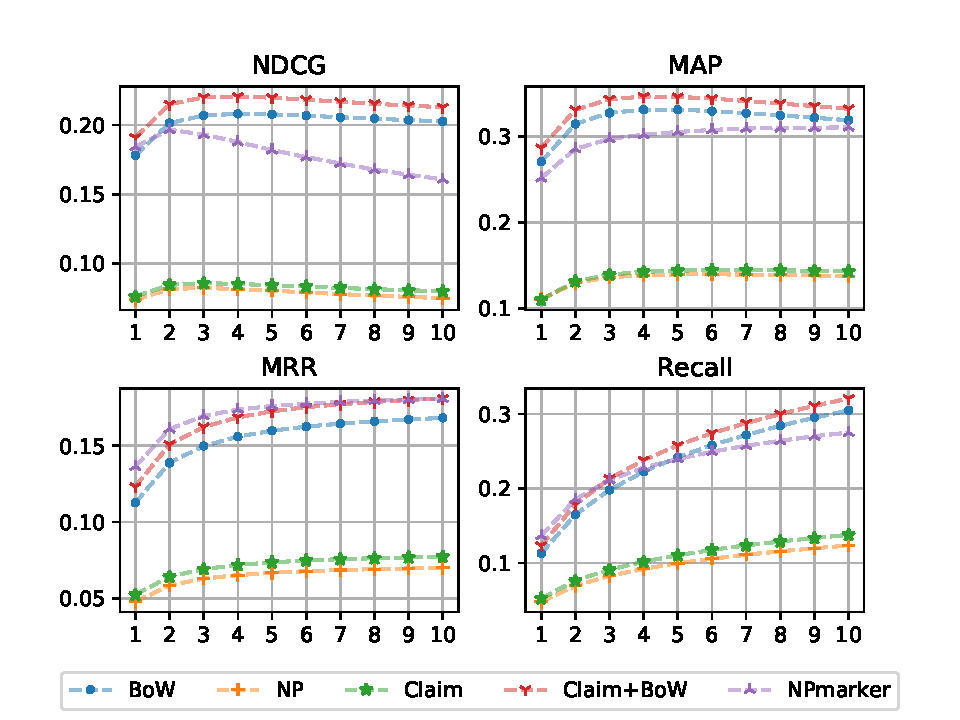
\includegraphics[width=.9\textwidth]{figures/evaluation/arXiv_CS_select.pdf}
  \caption{Evaluation using arXiv.}
  \label{fig:evalarxiv}
%\end{figure}

%\begin{figure}
  \centering
    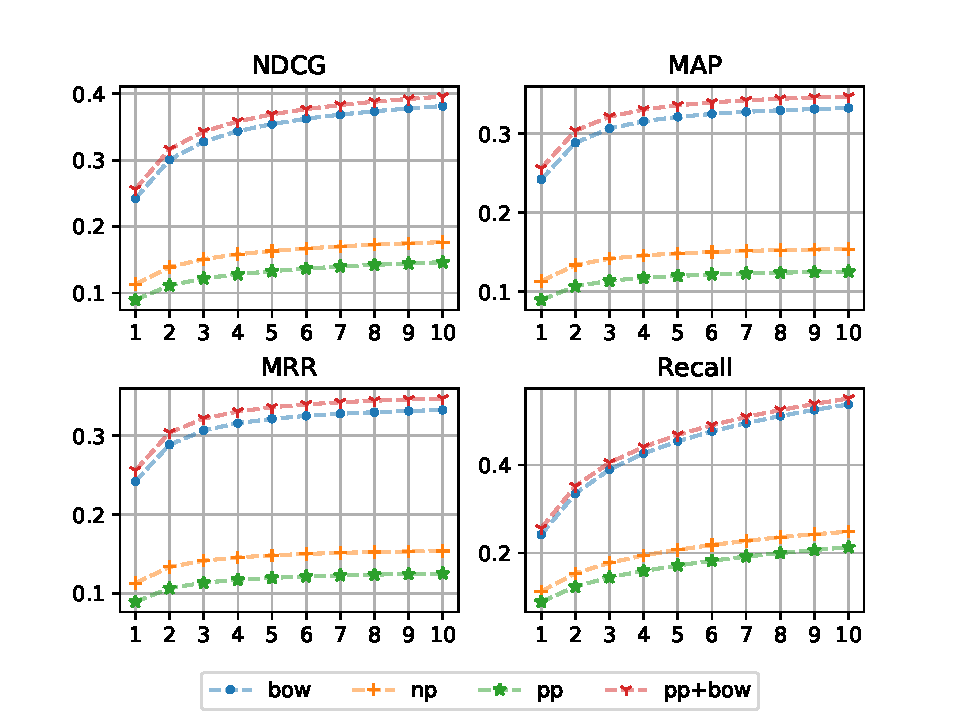
\includegraphics[width=.9\textwidth]{figures/evaluation/MAG_CS_es_wAbs_3M.pdf}
  \caption{Evaluation using the MAG.}
  \label{fig:evalmag}
\end{figure}

\begin{figure}
  \centering
    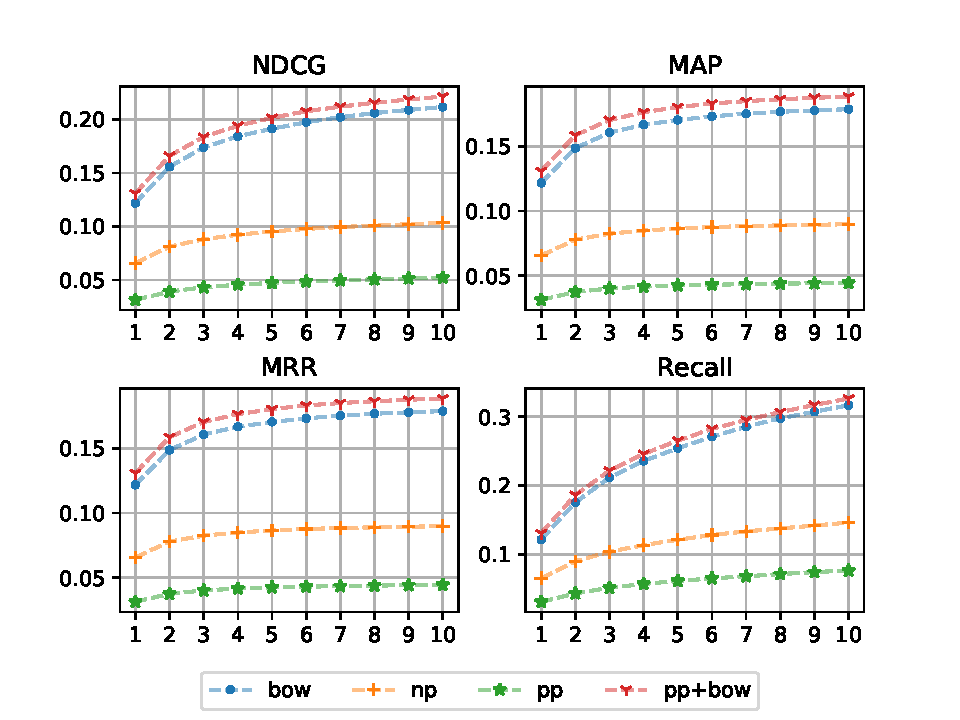
\includegraphics[width=.9\textwidth]{figures/evaluation/RefSeer.pdf}
  \caption{Evaluation using RefSeer.}
  \label{fig:evalrefseer}
%\end{figure}

%\begin{figure}
  \centering
    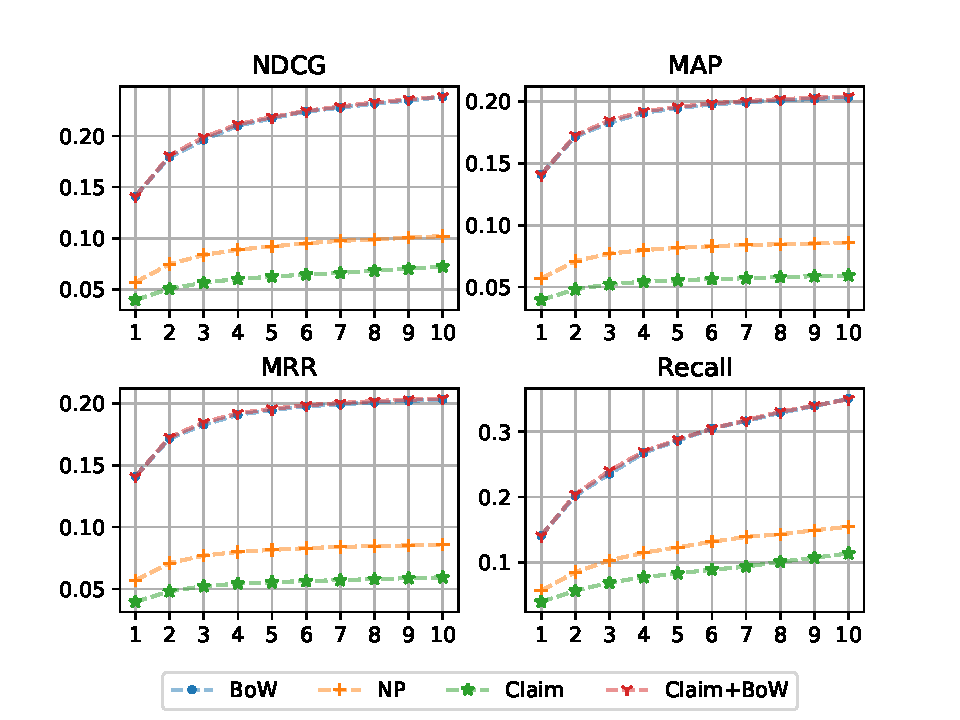
\includegraphics[width=.9\textwidth]{figures/evaluation/ACL.pdf}
  \caption{Evaluation using ACL-ARC.}
  \label{fig:evalacl}
\end{figure}

Figures~\ref{fig:evalarxiv}--\ref{fig:evalacl} show the results of these evaluations. For each of the data sets Claim+BoW outperforms the BoW baseline in each measure and for all cut-off values. Claim and NP do not compare in performance with the two aforementioned. This suggests that the claim structures we model with $R_{\text{claim}}$ are not enough for well performing recommendations on their own, but do capture information that non-semantic models (BoW) miss. NPmarker, only present in Figures~\ref{fig:evalarxiv}, gives particularly good results for lower cut-offs and performs especially well in the MRR metric. It performs the worst at high cut-offs measured by NDCG. Note that NPmarker is only evaluated for test set items where the model was applicable (i.e. where a noun phrase of minium length 2 is directly preceding the citation marker; cf. Section~\ref{sec:npmodel}). For our evaluation this was the case for 100,308 out of the 490,018 test set items (20.5\%). The evaluation results for NPmarker indicate that it is comparatively well suited to recommend citations where there is one particularly fitting publication (e.g. a reference paper for a tool, method or data set) and less suited for exemplifications (cf. Table~\ref{tab:citfunctions} in Chapter~\ref{chap:approach}). Comparing values between the different data sets, we can confirm our expectations based on the values in Table~\ref{tab:datasetprops}. For the MAG data, where we ensured very well described recommendation candidates by setting a threshold, the models perform best.
% Differences between the other three models are less straightforward, which is no surprise because there are many factors involved (number of recommendation candidates, number of contexts describing these, cleanliness of data, etc.).
This shows us that differences in data set composition can make a large difference in evaluation results. As a consequence, comparison between approaches is only realistically possible when using the same data.

% maybe mention \cite{Beel2017} ("None of these variations performed better than the simple out-of-the-box Apache Lucene baseline"), but then mention that Beel2017 is about *online* systems

% \cite{Huang2015} use CiteSeer (which RefSeer is based on) w/ 329,365 recommendation candidates. mby kind of comparable with a few buckets of salt?

\section{Online evaluation}\label{sec:oneval}
Main difference = direct human judgement

\subsection{Non-free text}
(i.e. insight into offline eval)
(controlled for free text input bias)

\subsection{Free text}
free free

    \chapter{Conclusion}\label{chap:conclusion}
looked into the use of explicit semantic representations for local citation recommendation.

(summary of methodology)

NPmarker performs best at low cut-offs and in MRR metric. Low cut-offs and measuring MRR can be interpreted as emulating a certain type of citation (i.e. citing reference publications). -> NPmarker is suited for such citations.

Citation type where a claim is backed by a citation can not really be emulated by cut-offs or choice of metric. Claim model relying on BoW "base" to outperform BoW at least suggests, that on it's own it is not very effective *generally* (for all citation types). Might be that also Claim model is well suited only for certain types of citations -> needs more investigation (see future work)

    \chapter{Future Work}\label{chap:todo}
% As a first step towards semantic citation recommendation, the work presented not only presents insights, but also lays bare new questions.
Several parts of the work presented merit continued development, others lay bare questions yet to be answered. In closing, we want to briefly highlight these with regards to the newly created data set, the entity as well as claim based models, and finally semantic citation recommendation in general.

The flexible nature of our data set makes it suitable for the development and evaluation of various citation based tasks, not just the one presented here. Because arXiv is an established resource in active use, new publications are added to it every day. These new submissions can be a valuable addition to our data set. In parallel to the development and evaluation of our models, we already extended the data with all publications from 2018~\cite{Saier2019}. Apart from the addition of new papers, the inclusion of mathematical formulas in some way, shape, or form (instead of replacing them with a substitution token) would presumably improve recommendation, as they can contain key information and are abundant in mathematics and physics papers. Such improvements can be guided by existing arXiv based efforts in mathematical information retrieval~\cite{Aizawa2014,Zanibbi2016}.

Because the arXiv data set spans several disciplines, a comparative analysis of the performance of our models could reveal interdisciplinary differences. As shown in our offline evaluation, the size and composition of a data set can have a large impact on the results. A comparative analysis would therefore require the adjustment of the data set's math and physics subsets in terms of number of recommendation candidates and number of citing papers describing those.

Concerning our NPmarker model, an evaluation on more than just the arXiv data is needed. Because the model relies on the exact position of the citation marker, which is not given in the other data sets used, a heuristic for the marker's identification could be tested. Another possibility would be the use of PMC-OAS data, as their JATS XML files also provide exact citation marker positions. Our Claim model in its current state uses the lemmatized form of predicates. These could be further generalized into a number of semantic relation types as done in~\cite{Gabor2018}. Given the model's current \emph{predicate-argument} structure, it might be possible to implement a basic semantic citation search on top of it, allowing users to, for example, search for publications showing that something \emph{``is:NP-hard''} or where the authors \emph{``improve:local citation recommendation''}. A last point concerning the claim based model is the realization of grammatical citation marker awareness. This requires proper handling of non-syntactic citations, which, judging by our user study results, make up the vast majority of citations. The algorithm presented in \cite{Abujbara2012} can be used as a starting point for identifying non-syntactic citations, but would have to be properly evaluated. The same holds true for their method of using the head of the nearest noun phrase as the new position of the marker.

Generally speaking, we think a more thorough and systematic examination of citation types---that is, structural types with respect to the grammatical and character-level location of information most descriptive of the cited document---should be a first step towards refining our existing models and creating new, citation type specific approaches.

In the long run, models revolving around claims could furthermore benefit from an assessment of credibility~\cite{Popat2016}; and beyond the level of claims, the modelling of argumentative structures, informed by existing work in the field of argumentation mining~\cite{Stab2016,Lippi2016,Habernal2017}, could enable even more refined recommendation results.


    % bibliography is not in the table of contents per default, add it manually
    % enable the \renewcommand for german header
    % \renewcommand{\bibname}{Literaturverzeichnis}
    \addcontentsline{toc}{chapter}{Bibliography}

    \bibliographystyle{ieeetr}
    \bibliography{bib/paper}

    \newpage  % makes Appendices page start at A1 instead of A3
    \pagenumbering{arabic}  % resets `page` counter to 1
    \renewcommand*{\thepage}{A\arabic{page}}
    \begin{appendices}
    \chapter{Evaluation of reference resolution}\label{chap:matcheval}

The sample of 300 matched reference items was acquired from the reference data base as shown in Listing~\ref{lst:matchevalsql}. The table \texttt{bibitem} holds most of the information on reference items. The table \texttt{bibitemmagidmap} contains per row the UUID of a reference item and the MAG ID it was matched to.

\begin{lstlisting}[caption={SQL query used to acquire the sample},label={lst:matchevalsql}]
select b.bibitem_string, m.mag_id
    from bibitem as b
        join
         (select *
            from bibitemmagidmap
                order by random()
                limit 300
         ) as m
        on b.uuid = m.uuid;
\end{lstlisting}

Table~\ref{tbl:matcheval} shows the full evaluation. Wrongly matched items are {\color{UniRed}highlited in red}. Note that there are seven cases where the reference item refers to more than one publication. In such cases our method only captures the first one and is cosequetually evaluated on the first one. Note further that in one case a reference item named a PhD thesis while the match was for the very same thesis published two years later. This was deemed a correct match. Lastly, there was one case where a book was cited with the date indicating its second edition while the matched record in the MAG has a date indiciating the books thrid edition. This also was deemed a correct match.
\newpage

\tiny
\begin{longtable}{m{11.4cm}@{\hspace{0.2in}}c@{\hspace{0.2in}}c}
\caption{Evaluation}\label{tbl:matcheval}\\
\toprule
    Reference item & MAG ID & \hphantom{ }\\
\midrule
    V. N. Senoguz and Q. Shafi, “Reheat temperature in supersymmetric hybrid inflation models,” Phys. Rev. D 71, 043514 (2005) [hep-ph/0412102]. & 2075392245 & \checkmark \\
    Keiding, N. and Nielsen, J.E. (1975) Branching processes with varying and random geometric offspring distributions. J. Appl. Prob. 12, 135–141. & 2332540167 & \checkmark \\
    H. Izeki and S. Nayatani, Combinatorial harmonic maps and discrete-group actions on Hadamard spaces, Geom. Dedicata 114 (2005), 147–188. & 2017711173 & \checkmark \\
    T. Adamo, M. Bullimore, L. Mason and D. Skinner, “Scattering Amplitudes and Wilson Loops in Twistor Space,” J. Phys. A 44 (2011) 454008 [arXiv:1104.2890 [hep-th]]. & 2002091616 & \checkmark \\
    Eren Mehmet Kıral and Matthew Young, The fifth moment of modular FORMULA -functions, arXiv preprint arXiv:1701.07507 (2017). & 2582886839 & \checkmark \\
    T. Baumgarte and S. Shapiro, Numerical Relativity: Solving Einstein's Equations on the Computer. Cambridge University Press, 2010. http://books.google.co.uk/books?id=dxU1OEinvRUC. & 2566410267 & \checkmark \\
    R.E. Renfordt, D. Schall, R. Bock, R. Brockmann, J.W. Harris, A. Sandoval, R. Stock, H. Ströbele, D. Bangert, W. Rauch, G. Odyniec, H.G. Pugh, and L.S. Schroeder, Phys. Rev. Lett. 53 (1984) 763. & 2001418221 & \checkmark \\
    T. A. Porter, I. V. Moskalenko, A. W. Strong, E. Orlando and L. Bouchet, arXiv:0804.1774 [astro-ph]. & 2129746122 & \checkmark \\
    Jon Kleinberg, Sendhil Mullainathan, and Manish Raghavan. Inherent trade-offs in the fair determination of risk scores. arXiv preprint arXiv:1609.05807, 2016. & 2522104760 & \checkmark \\
    R.M. Fernandes, L. H. VanBebber, S. Bhattacharya, P. Chandra, V. Keppens, D. Mandrus, M.A. McGuire, B.C. Sales, A.S. Sefat, and J. Schmalian, Phys. Rev. Lett. 105, 157003 (2010) & 2143202785 & \checkmark \\
    Fomin, S., Wei, P., Chugunov, V., 1995. Contact melting by a non-isothermal heating surface of arbitrary shape. Int. J. Heat Mass Transfer 38 (17), 3275–3284. & 2030656707 & \checkmark \\
    R.F. Lebed, arXiv:1507.05867v1 [hep-ph]. & 1844403609 & \checkmark \\
    R. Billinton, R. Karki, Y. Gao, D. Huang, P. Hu, and W. Wangdee, “Adequacy Assessment Considerations in Wind Integrated Power Systems,” IEEE Trans. Power Syst., vol. 27, no. 4, pp. 2297–2305, 2012. & 2024825567 & \checkmark \\
    C. Morningstar and M. Peardon, Phys. Rev. D 56, 4043 (1997). & 2109255696 & \checkmark \\
    I. B. S. Passi, M. Singh and M. K. Yadav, Automorphisms of abelian group extensions, J. Algebra 324 (2010), 820–830. & 2051680489 & \checkmark \\
    S. Dimopoulos, P. W. Graham, J. M. Hogan, M. A. Kasevich, and S. Rajendran, Phys. Rev. D 78, 122002 (2008). & 2749889157 & \checkmark \\
    P.Jaworski, Value at Risk in the presence of the power laws, Acta Physica Polonica B 36 (2005) 2575-2587. & 2566822874 & \checkmark \\
    L. L. Chau, M. L. Ge and Y. S. Wu, Phys. Rev. D 25, 1086 (1982); L. L. Chau and Wu Yong-Shi, Phys. Rev. D 26, 3581 (1982); L. L. Chau, M. L. Ge, A. Sinha and Y. S. Wu, Phys. Lett. B 121, 391 (1983). & 2075757391 & \checkmark \\
    E. C. Blomberg, M. a. Tanatar, R. M. Fernandes, I. I. Mazin, B. Shen, H.-H. Wen, M. D. Johannes, J. Schmalian, and R. Prozorov, Nat. Commun. 4, 1914 (2013). & 2081425933 & \checkmark \\
    A. Arenas, A. Díaz-Guilera, C. J. Pérez-Vicente, Synchronization reveals topological scales in complex networks, Phys. Rev. Lett. 96 (11) (2006) 114102. & 2100240966 & \checkmark \\
    M. Alizadeh, A. Greenberg, D. A. Maltz, J. Padhye, P. Patel, B. Prabhakar, S. Sengupta, and M. Sridharan. Data Center TCP (DCTCP). ACM SIGCOMM, 2010. & 2164740236 & \checkmark \\
    M. Nishiyama, T. Okabe, Y. Sato, and I. Sato. Sensation-based photo cropping. In ACM Multimedia, pages 669–672, 2009. & 2013339738 & \checkmark \\
    L. Landau and E. Lifchitz, Classical theory of fields, Butterworth-Heinemann, Oxford, 1994, p. 87. & 119088996 & \checkmark \\
    Peregrine, D., 2003. Water-wave impact on walls. Annu. Rev. Fluid Mech. 35, 23--43. & 2118259172 & \checkmark \\
    M. S. Khalil, S. Gladchenko, M. J. A. Stoutimore, F. C. Wellstood, A. L. Burin, and K. D. Osborn, Phys. Rev. B 90, 100201 (2014). & 1998393159 & \checkmark \\
    F. Gabbiani, E. Gabrielli, A. Masiero and L. Silvestrini, Nucl. Phys. B 477, 321 (1996) [arXiv:hep-ph/9604387]. & 2133327165 & \checkmark \\
    Abramowitz, M. and Stegun, I. A., Handbook of Mathematical Functions, (Dover, New York, 1965). & 2120062331 & \checkmark \\
    N. V. Chawla, K. W. Bowyer, L. O. Hall, and W. P. Kegelmeyer. Smote: synthetic minority over-sampling technique. Journal of artificial intelligence research, 16(1):321–357, 2002. & 2148143831 & \checkmark \\
    B. H. Lee, W. Lee, R. MacKenzie, M. B. Paranjape, U. A. Yajnik and D. h. Yeom, Phys. Rev. D 88, 085031 (2013). & 2074315988 & \checkmark \\
    D. Nishiguchi, K. H. Nagai, H. Chaté, and M. Sano, Long-range nematic order and anomalous fluctuations in suspensions of swimming filamentous bacteria. arXiv preprint arXiv:1604.04247 (2016). & 2336881770 & \checkmark \\
    Huelga, S. F. et al., Improvement of frequency standards with quantum entanglement. Phys. Rev. Lett. 79, 3865 (1997). & 2015876000 & \checkmark \\
    M. Henneaux and C. Teitelboim, Asymptotically anti-de Sitter spaces, Comm. Math. Phys. 98, 391 (1985). & 2134856726 & \checkmark \\
    D. Boucher, W. Geiselmann, and F. Ulmer, Skew-cyclic codes, Applicable Algebra in Engineering, Communication and computing, (18) (4), (2007), 379-389. & 2151359594 & \checkmark \\
    R. C. Brower, H. Nastase, H. J. Schnitzer and C.-I. Tan, arXiv:0801.3891 [hep-th]. & 1995185450 & \checkmark \\
    S. Sarkar, Big bang nucleosynthesis and physics beyond the standard model, Rept. Prog. Phys. 59 (1996) 1493–1610, [hep-ph/9602260]. & 2013442457 & \checkmark \\
    M. Iskin and J. K. Freericks, Phys. Rev. A 80, 053623 (2009). & 2076979008 & \checkmark \\
    M. L. Skoge \& T. W. Baumgarte, Phys. Rev. D 66 107501 (2002). & 2016175541 & \checkmark \\
    A. Lozano, A. M. Tulino, and S. Verdú, “Optimum power allocation for parallel Gaussian channels with arbitrary input distributions,” IEEE Trans. Inf. Theory, vol. 52, no. 7, pp. 3033–3051, Jul. 2006. & 2097695636 & \checkmark \\
    F. Paci, A. Gruppuso, F. Finelli, A. De Rosa, N. Mandolesi, and P. Natoli, MNRAS 434, 3071 (Oct. 2013), arXiv:1301.5195 & 1976439668 & \checkmark \\
    Samuel Brody and Noemie Elhadad. 2010. An unsupervised aspect-sentiment model for online reviews. In Human Language Technologies: The 2010 Annual Conference of the North American Chapter of the Association for Computational Linguistics, pages 804–812. Association for Computational Linguistics. & 2113786470 & \checkmark \\
    R. Islam, C. Senko, W. C. Campbell, S. Korenblit, J. Smith, A. Lee, E. E. Edwards, C.-C. J. Wang, J. K. Freericks, and C. Monroe, Emergence and frustration of magnetism with variable-range interactions in a quantum simulator, Science 340, 583 (2013). & 1606923443 & \checkmark \\
    I. Ermolli, K. Matthes, T. Dudok de Wit, N.A. Krivova, K. Tourpali, M. Weber, Y.C. Unruh, L. Gray, U. Langematz, P. Pilewskie, E. Rozanov, W. Schmutz, A. Shapiro, S.K. Solanki, T.N. Woods, Recent variability of the solar spectral irradiance and its impact on climate modelling. Atmos. Chem. Phys. 13, 3945–3977 (2013). doi:10.5194/acp-13-3945-2013 & 2158950390 & \checkmark \\
    Tauchen G. and Zhou, H. (2011), “Realized Jumps on Financial Markets and Predicting Credit Spreads,” Journal of Econometrics, 160, 102–118 & 2113380547 & \checkmark \\
    S. Yoon, W. Ye, J. Heidemann, B. Littlefield, and C. Shahabi. Swats: Wireless sensor networks for steamflood and waterflood pipeline monitoring. Network, IEEE, 25(1):50–56, January 2011. & 2054094122 & \checkmark \\
    J.Y. Vaishnav and C.W. Clark, Phys. Rev. Lett. 100, 153002 (2008). & 2752272568 & \checkmark \\
    L. J. Hall, T. Moroi and H. Murayama, Phys. Lett. B 424, 305 (1998). [arXiv:hep-ph/9712515]. & 2078593377 & \checkmark \\
    Movassaghi, Samaneh and Abolhasan, Mehran and Smith, David, Smart spectrum allocation for interference mitigation in Wireless Body Area Networks, IEEE International Conference on Communications (ICC), pages 5688-5693, 2014 & 2083602816 & \checkmark \\
    M. Apollonio et al. [CHOOZ Collaboration], Phys. Lett. B 466, 415 (1999) [arXiv:hep-ex/9907037]. & 1571701324 & \checkmark \\
    G. 't Hooft, “Magnetic Monopoles in Unified Gauge Theories,” Nucl.Phys. B79 (1974) 276–284. & 2027710569 & \checkmark \\
    D. C. Cabra, M. D. Grynberg, P. C. W. Holdsworth, A. Honecker, P. Pujol, J. Richter, D. Schmalfß, and J. Schulenburg, Phys. Rev. B 71, 144420 (2005). & 2032654705 & \checkmark \\
    V.A. Dolgushev, Erratum to: ""A Proof of Tsygan's Formality Conjecture for an Arbitrary Smooth Manifold"", arXiv:math/0703113. & 132267651 & \checkmark \\
    {\color{UniRed}Eddy, J.A.: 1983, The maunder minimum - a reappraisal. Solar Phys. 89, 195. ADS.} & {\color{UniRed}2024069573} & {\color{UniRed}$\times$} \\
    Bouliotis, G. and Billingham, L. (2011) Crossing survival curves: alternatives to the log-rank test. Trials, 12, 1. & 2136058878 & \checkmark \\
    I. Peschel and V. Eisler, Reduced density matrices and entanglement entropy in free lattice models, J. Phys. A 42 504003 (2009). & 2141130841 & \checkmark \\
    C. Gundlach, Critical phenomena in gravitational collapse, submitted to Adv. Theor. Math. Phys., preprint gr-qc/9712084. & 2103342599 & \checkmark \\
    A. Blumen, G. Zumofen, and J. Klafter, Target annihilation by random walkers, Phys. Rev. B 30, 5379 (1984). & 2060897997 & \checkmark \\
    M. Alidoust, K. Halterman, and J. Linder, Phys. Rev. B 89, 054508 (2014). & 2012436162 & \checkmark \\
    G. Ciavola, L. Celona, S. Gammino, M. Presti, L. Ando, S. Passarello, X.Zh. Zhang, F. Consoli, F. Chines, C. Percolla, V. Calzona and M. Winkler, A version of the Trasco Intense Proton Source optimized for accelerator driven system purposes. Rev. Sci. Instrum. 75 (2004) 1453–1456,. & 2075428341 & \checkmark \\
    D.Litim Phys. Rev. Lett. 92 (2004) 201301, hep-th/0312114 & 2000661521 & \checkmark \\
    P.K. Kovtun, D.T. Son, and A.O. Starinets, Phys. Rev. Lett. 94, 111601 (2005). & 2097909025 & \checkmark \\
    Jones, J. A. et al. Magnetic Field Sensing Beyond the Standard Quantum Limit Using 10-Spin NOON States. Science 324, 1166–1168 (2009). & 2022149792 & \checkmark \\
    G.E.Brown and M.Rho, Phys.Rev.Lett. 66, (1991) 2720; & 1971702030 & \checkmark \\
    K. Banaszek and K. Wódkiewicz, “Operational theory of homodyne detection,” Phys. Rev. A 55, 3117 (1997). & 1985850877 & \checkmark \\
    Barbara Di Eugenio, Pamela W. Jordan, and Liina Pylkkänen. 1998. The COCONUT project: Dialogue annotation manual. Technical Report 98-1, University of Pittsburgh, Intelligent Systems Program. [www.isp.pitt.edu/intgen/coconut.html]. & 116082719 & \checkmark \\
    Beirlant, J., Y. Goegebeur, J. Segers, and J. Teugels (2004). Statistics of extremes: Theory and Applications. Wiley Series in Probability and Statistics. Chichester: John Wiley \& Sons Ltd. & 1598342322 & \checkmark \\
    Guillaumin, M., Mensink, T., Verbeek, J.J., Schmid, C.: Tagprop: Discriminative metric learning in nearest neighbor models for image auto-annotation. In: IEEE 12th International Conference on Computer Vision, ICCV 2009, Kyoto, Japan, September 27 - October 4, 2009. (2009) 309–316 & 2536305071 & \checkmark \\
    T. Faulkner et al., “Gravitation from entanglement in holographic CFTs,” (2013), arXiv:1312.7856v1. & 2102970467 & \checkmark \\
    René Thom, Quelques propriétés globales des variétés différentiables, Comment. Math. Helv. 28 (1954), 17–86. & 1989427081 & \checkmark \\
    A. Schikorra. Regularity of n/2-harmonic maps into spheres. PhD-Thesis, arXiv:1003.0646v1, 2010. & 2029831933 & \checkmark \\
    M. J. Simpson, J. A. Sharp, and R. E. Baker. Survival probability for a diffusive process on a growing domain. Phys. Rev. E 91, 042701 (2015). & 1988447698 & \checkmark \\
    D. Bergamini, N. Descoubes, C. Joubert \& R. Mateescu (2005): Bisimulator: A Modular Tool for On-the-Fly Equivalence Checking. In: Proc. of TACAS'05, Lecture Notes in Computer Science 3440, Springer-Verlag, pp. 581–585. & 1503429725 & \checkmark \\
    J. A. Baldwin, O. Plamenevskaya, Khovanov homology, open books, and tight contact structures. math.GT/0808.2336 & 2054234174 & \checkmark \\
    Eisenberger, P., et al., 1972, Phys. Rev. B 6, 3671. & 1980522055 & \checkmark \\
    O. Viehmann, C. Eltschka, and J. Siewert, Appl. Phys. B 106, 533 (2012). & 2076107066 & \checkmark \\
    A. Rényi. Representations for real numbers and their ergodic properties. Acta Math. Acad. Sci. Hungar 8 (1957), 477–493. & 2089164015 & \checkmark \\
    D. Chicharro and R. G. Andrzejak, Phys. Rev. E 80, 026217 (2009). & 2078979753 & \checkmark \\
    Kenward, M. G., Jones, B., 1992. Alternative approaches to the analysis of binary and categorical repeated measurements. Journal of Biopharmaceutical Statistics 2 (2), 137–170. & 1967449535 & \checkmark \\
    J. Nešetřil and V. Rödl. The partite construction and Ramsey set systems. Discrete Mathematics, 75(1-3):327–334, 1989. & 2062861878 & \checkmark \\
    E. Seiler, Gauge Theories as a Problem of Constructive Quantum Field Theory and Statistical Mechanics, Lecture Notes in Physics Vol. 159 (Springer, Berlin, 1982). & 1608098855 & \checkmark \\
    M. Gaye, Y. Chitour, and P. Mason. Properties of barabanov norms and extremal trajectories associated with continuous-time linear switched systems. In Proceedings of the 52nd IEEE Conference on Decision and Control, pages 716–721, Florence, Italie, 2013. & 2090302562 & \checkmark \\
    Kováčik R. and Ederer C., Phys. Rev. B 80 (2009) 140411; Kim M. et al., Phys. Rev. B 81 (2010) 100409. & 1758648405 & \checkmark \\
    Morandi, G., Ferrario, C., Lo Vecchio, G., Marmo, G. and Rubano, C. (1990). The inverse problem in the calculus of variations and the geometry of the tangent bundle, Phys. Rep. 188, 147. & 2026992500 & \checkmark \\
    G. Da Prato and J. Zabczyk, Ergodicity for infinite dimensional systems, London Mathematical Society Lecture Note Series, 229, Cambridge University Press, 1996. & 1530927473 & \checkmark \\
    R. Trotta, Bayes in the sky: Bayesian inference and model selection in cosmology, Contemp. Phys. 49 (2008) 71–104, [arXiv:0803.4089]. & 2021748112 & \checkmark \\
    Christof, J., M. Gebhardt, A. E.-M. Clemen, J. Jaud, , and M. Rief, 2006. Myosin-V is a mechanical ratchet. Proc. Natl. Acad. Sci. U.S.A. 103:8680–8685. & 2095633207 & \checkmark \\
    G.M. Molchan: Burgers equation with self-similar Gaussian initial data: tail probabilities. J. of Stat. Phys. 88 (1997) 1139–1150. & 2000957076 & \checkmark \\
    Arata, I., Y. Ohno, F. Matsukura, and H. Ohno, 2001, “Temperature dependence of electroluminescence and I-V characteristics of ferromagnetic/non-magnetic semiconductor pn junctions,” Physica E 10, 288–291. & 1987870048 & \checkmark \\
    I. Zlatev, L. Wang and P.J. Steinhardt, Phys. Rev. Lett. 82, 896 (1999); Phys. Rev. D 59, 123504 (1999). & 2032901690 & \checkmark \\
    A. Valentini, in: Bohmian Mechanics and Quantum Theory: an Appraisal, eds. J. T. Cushing et al. (Kluwer, Dordrecht, 1996). & 207861407 & \checkmark \\
    R. Killip, S. Kwon, S. Shao, and M. Visan. On the mass-critical generalized KdV equation. Discrete Contin. Dyn. Syst., 32(1):191–221, 2012. & 1975802612 & \checkmark \\
    Danilo Jimenez Rezende and Shakir Mohamed. Variational inference with normalizing flows. arXiv preprint arXiv:1505.05770, 2015. & 299440670 & \checkmark \\
    D. Rossi and G. Rossini, “On sizing CCN content stores by exploiting topological information,” in Proc. IEEE NOMEN, 2012. & 1985355206 & \checkmark \\
    F. Bezrukov, A. Magnin, M. Shaposhnikov and S. Sibiryakov, JHEP 1101 (2011) 016 [arXiv:1008.5157]. & 2064410211 & \checkmark \\
    M. Horodecki, P. Horodecki, and R. Horodecki. Separability of mixed quantum states: linear contractions approach. preprint archiv quant-ph/0206008. & 1668368460 & \checkmark \\
    S. White, Phys. Rev. B 48, 10345 (1993). & 2016407890 & \checkmark \\
    A. Brandt et al., [UA8 Collaboration], Evidence for a Super-Hard Pomeron Structure, submitted to Phys. Lett. 1992. & 1983143801 & \checkmark \\
    Fan, T.-H. \& Berger, J. O. (2000). Robust Bayesian displays for standard inferences concerning a normal mean. Computational Statistics \& Data Analysis 33 381–399. & 2030654698 & \checkmark \\
    S. Ryu, J. E. Moore, and A. W. W. Ludwig, Phys. Rev. B 85, 045104 (2012), arXiv:1010.0936. & 2083123179 & \checkmark \\
    P. Balaz, V. K. Dugaev, and J. Barnaś Phys. Rev. B 85, 024416 (2012) & 2322343165 & \checkmark \\
    T. Giamarchi and A. Tsvelik, Phys. Rev. B 59, 11398 (1999). & 2069018114 & \checkmark \\
    M. Molloy and B. Reed. The size of the giant component of a random graph with a given degree sequence. Combin. Probab. Comput., 7(3):295–305, (1998). & 2129918926 & \checkmark \\
    D. W. Sivers, Phys. Rev. D 41, 83 (1990); Phys. Rev. D 43, 261 (1991). & 2174029682 & \checkmark \\
    J. Boronat and J. Casulleras, Phys. Rev. B 49, 8920 (1994). & 1982967539 & \checkmark \\
    J. N. Bandyopadhyay and A. Lakshminarayan, Phys. Rev. E 69, 016201 (2004). & 1977839735 & \checkmark \\
    Priest ER, Forbes TG (2002) The magnetic nature of solar flares. 10:313–377, DOI 10.1007/s001590100013 & 2014209718 & \checkmark \\
    W. Woerndl, C. Schueller, and R. Wojtech. A hybrid recommender system for context-aware recommendations of mobile applications. In Proceedings of ICDEW '07, pages 871–878, Washington, DC, USA, 2007. IEEE Computer Society. & 2112166834 & \checkmark \\
    {[auto:STB|2013/06/05|13:45:01]} Worsley, K. J.K. J., Liao, C. H.C. H., Aston, J.J., Petre, V.V., Duncan, G. H.G. H., Morales, F.F. Evans, A. C.A. C. (2002). A general statistical analysis for fMRI data. NeuroImage 15 1–15. imsref & 1975938737 & \checkmark \\
    L.H. Ford and N.F. Svaiter, Phys. Rev. D 58, 065007 (1998), quant-ph/9804056. & 1963985219 & \checkmark \\
    H. Häffner, S. Gulde, M. Riebe, G. Lancaster, C. Becher, J. Eschner, F. Schmidt-Kaler, R. Blatt, Precision measurement and compensation of optical Stark shifts for an ion-trap quantum processor, Phys. Rev. Lett. 90 (2003) 143602. & 2129198554 & \checkmark \\
    I. Jeon, K. Lee, J.-H. Park, and Y. Suh, Stringy Unification of Type IIA and IIB Supergravities under N=2 D=10 Supersymmetric Double Field Theory, Phys.Lett. B723 (2013) 245–250, [arXiv:1210.5078]. & 1967998606 & \checkmark \\
    Z.A. Anastassi and T.E. Simos: A Trigonometrically-Fitted Runge-Kutta Method for the Numerical Solution of Orbital Problems, New Astronomy, 10, 301-309 (2005) & 2024993485 & \checkmark \\
    Fletcher, A. 2010, in Astronomical Society of the Pacific Conference Series, Vol. 438, The Dynamic Interstellar Medium: A Celebration of the Canadian Galactic Plane Survey, ed. R. Kothes, T. L. Landecker, \& A. G. Willis, 197 & 1671679100 & \checkmark \\
    V. A. Belinsky, I. M. Khalatnikov, and E. M. Lifshitz. Oscillatory approach to a singular point in the relativistic cosmology. Adv. Phys., 19:525–573, 1970. & 2048737175 & \checkmark \\
    Allen, D. A. et al., 1993. IRIS – an Infrared Imager and Spectrometer for the Anglo-Australian Telescope. Proceedings of the Astronomical Society of Australia 10, 298. & 91162570 & \checkmark \\
    D. Cooper, Automorphisms of free groups have finitely generated fixed point sets. J. Algebra, 111 (1987), no. 2 453–456 & 2076181847 & \checkmark \\
    J.-L. Lehners and P. J. Steinhardt, “Intuitive understanding of non-gaussianity in ekpyrotic and cyclic models,” Phys.Rev. D78 (2008) 023506, arXiv:0804.1293 [hep-th]. & 2592352904 & \checkmark \\
    Z.-B. Wu, Global transposable characteristics in the complete DNA sequence of the yeast. Physica A 389 (2010) 5698. & 1548592618 & \checkmark \\
    E. Nowak, F. Jurie, and B. Triggs. Sampling strategies for bag-of-features image classification. In Computer Vision–ECCV 2006, pages 490–503. Springer, 2006. & 2171896402 & \checkmark \\
    Benjamin C. Pierce. Types and programming languages: The next generation. LICS'03, 2003. & 1951034176 & \checkmark \\
    G. Tardos and G. Tóth. Multiple coverings of the plane with triangles. Discrete \& Computational Geometry, 38(2):443–450, 2007. & 2043718124 & \checkmark \\
    T. Rivière, Analysis aspects of Willmore surfaces, Invent. Math., Vol. 174, (2008), 1–45. & 1606077524 & \checkmark \\
    H. Mabuchi, Phys. Rev. A 85, 015806 (2012). & 1620088716 & \checkmark \\
    I. Schienbein, J. Y. Yu, K. Kovarik, C. Keppel, J. G. Morfin, F. Olness and J. F. Owens, Phys. Rev. D 80, 094004 (2009) & 2050053974 & \checkmark \\
    D.Q. Goldin, S.A. Smolka, P.C. Attie, E.L. Sonderegger, Turing machines, transition systems and interaction, manuscript, 2003. & 2048671682 & \checkmark \\
    P. Collet and J.P. Eckmann, Iterated Maps on the Interval as Dynamical Systems, (Birkhäuser, Basel, 1980). & 1573241742 & \checkmark \\
    M. F. Maghrebi, R. L. Jaffe, and M. Kardar, Phys. Rev. Lett. 108, 230403 (2012). & 2025571896 & \checkmark \\
    A. Minami and A. Onuki, Phys. Rev. B 70, 184114 (2004); Acta Mater. 55, 2375 (2007). & 1514590689 & \checkmark \\
    Kfir Blum, Anson Hook, and Kohta Murase, “High energy neutrino telescopes as a probe of the neutrino mass mechanism,” (2014), arXiv:1408.3799 [hep-ph] . & 1628049864 & \checkmark \\
    O. E. Buryak, Phys. Rev. D 53 (1996) 1763 [gr-qc/9502032]. & 2069968655 & \checkmark \\
    Kolb, E. W.; Turner, M. S. The Early Universe, AddisonWesley Publishing Company: California, USA, 1990. & 2595419339 & \checkmark \\
    G. Binasch, P. Grünberg, F. Saurenbach, and W. Zinn, Phys. Rev. B 39, 4828 (1989). & 2043072234 & \checkmark \\
    JC Baygents and DA Saville. The circulation produced in a drop by an electric field: a high field strength electrokinetic model. In AIP Conference Proceedings, volume 197, pages 7–17. AIP, 1990. & 1612371284 & \checkmark \\
    E. Altman and R. Vosk, Annual Review of Condensed Matter Physics 6, 383 (2015). & 2166587989 & \checkmark \\
    J.-M. Souriau, Structure des systèmes dynamiques (Dunod, 1970). & 108534386 & \checkmark \\
    F. Horn. Explicit Muller games are PTIME. In Proc. 28th Conference on Foundations of Software Technology and Theoretical Computer Science (FSTTCS'08), LIPIcs 2, p. 235–243. Leibniz-Zentrum für Informatik, 2008. & 2240543079 & \checkmark \\
    A. G. Izergin and V. E. Korepin, “The Inverse Scattering Method Approach To The Quantum Shabat-Mikhailov Model,” Commun. Math. Phys. 79 (1981) 303. & 1977168974 & \checkmark \\
    Balzano, V. A. 1983 Star-burst Galactic Nuclei. ApJ 268, 602–627. & 2059760395 & \checkmark \\
    M. Ishak, A. Upadhye, D. N. Spergel, Phys. Rev. D 74, 043513 (2006) [arXiv:astro-ph/0507184]. & 2044422425 & \checkmark \\
    M. Lynker and R. Schimmrigk, Landau–Ginzburg theories as orbifolds, Phys. Lett. B249 (1990) 237 & 2030907161 & \checkmark \\
    S. T. Petcov, T. Shindou and Y. Takanishi, Nucl. Phys. B 738, 219 (2006) [arXiv:hep-ph/0508243]. & 2007551251 & \checkmark \\
    J. E. Lye, L. Fallani, C. Fort, V. Guarrera, M. Modugno, D. S. Wiersma, and M. Inguscio, Phys. Rev. A 75, 061603(R) (2007). & 2015993116 & \checkmark \\
    J. P. Perdew, K. Burke, and M. Ernzerhof, Phys. Rev. Lett. 77, 3865 (1996). & 1981368803 & \checkmark \\
    J. F. Clauser, M. A. Horne, A. Shimony, and R. A. Holt, Physical Review Letters 23, 880 (1969), URL http://doi.org/10.1103/PhysRevLett.23.880. & 2028815089 & \checkmark \\
    M. Horodecki and P. Horodecki, Phys. Rev. A 59, 4206 (1999). & 2000407553 & \checkmark \\
    B. Mazur, Rational isogenies of prime degree. Invent. Math. 44 (1978), 129–162. & 2011844852 & \checkmark \\
    Arnold, B.C, Balakrishnan, N., Nagaraja H.N., (1992), A First course in order statistics, Wiley and sons. & 2318245334 & \checkmark \\
    K. Bamba and S. D. Odintsov, JCAP 0804, 024 (2008) [arXiv:0801.0954 [astro-ph]]. & 2065428968 & \checkmark \\
    Mujherjee N. P. and Bhattacharya, P., Fuzzy Groups Some Group-Theoretic Analogs, Information Science39,247-268 (1986). & 1999360086 & \checkmark \\
    Karen Suzanne Oberhauser, M. J. S. The monarch butterfly: biology and conservation. Cornell university press, 2004. & 570971783 & \checkmark \\
    A. Belloni, V. Chernozhukov, and C. Hansen. Inference for high-dimensional sparse econometric models. Advances in Economics and Econometrics: The 2010 World Congress of the Econometric Society, 3:245–295, 2013. & 1720842782 & \checkmark \\
    M. I. Aroyo, A. Kirov, C. Capillas, J. M. Perez-Mato, and H. Wondratschek, Acta Cryst. A 62, 115 (2006b). & 1996820002 & \checkmark \\
    V. Del Duca and C. R. Schmidt, Dijet Production At Large Rapidity Intervals, 4919944510 [9311290]. & 2003427747 & \checkmark \\
    G. F. Giudice and A. Strumia, Nucl. Phys. B 858 (2012) 63 [arXiv:1108.6077 [hep-ph]]. & 2015208992 & \checkmark \\
    C. D. Herrera, J. Kannala, P. Sturm, and J. Heikkila. A learned joint depth and intensity prior using markov random fields. In 3DTV-Conference, 2013 International Conference on, pages 17–24. IEEE, 2013. & 1994295411 & \checkmark \\
    {\color{UniRed}J. Zhu, S. Rosset, T. Hastie, and R. Tibshirani. 1-norm support vector machines. In Advances in Neural Information Processing Systems (NIPS), volume 16, pages 49–56, 2004.} & {\color{UniRed}2249237221} & {\color{UniRed}$\times$} \\
    M. Beynon, B. Curry, and P. Morgan, ""The Dempster-Shafer theory of evidence:an alternative approach to multicriteria decision modelling"", Omega, vol. 28, no. 1, pp. 37–50, 2000. & 2121042048 & \checkmark \\
    S. Flach, M. V. Ivanchenko, and O. I. Kanakov, Phys. Rev. Lett. 95, 064102/1-4 (2005). & 2004622729 & \checkmark \\
    P. Carrasco, A. M. Cegarra, and A. R. Garzon. Nerves and classifying spaces for bicategories, 2010. & 2108966476 & \checkmark \\
    R. Sandhu, S. Dambreville, A. Tannenbaum, Particle Filtering for Registration of 2D and 3D Point Sets with Stochastic Dynamics. Pro. of IEEE Conference on Computer Vision and Pattern Recognition, 2008, pp. 1-8. & 2146847221 & \checkmark \\
    S. Ji, Y. Xue and L. Carin, “Bayesian compressive sensing,” IEEE Trans. Signal Process., vol. 56, no. 6, pp. 2346–2356, 2008. & 2071284784 & \checkmark \\
    Jun Li. A degeneration formula of GW-invariants. J. Differential Geom., 60(2):199–293, 2002. & 1484479264 & \checkmark \\
    J. Milnor, Dynamics in One Complex Variable, Vieweg, Göttingen, 2000. & 1603977374 & \checkmark \\
    Marcheselli, M., Baccini, A. and Barabesi, L.  (2008). Parameter estimation for the discrete stable family. Communications in Statistics - Theory and Methods 37 815–830. & 2035009392 & \checkmark \\
    A. Chantasri, J. Dressel, and A. N. Jordan, Action principle for continuous quantum measurement, Phys. Rev. A 88, 042110 (2013). & 2025224750 & \checkmark \\
    A. Strominger, Black hole entropy from near horizon microstates, JHEP 9802 (1998) 009, [hep-th/9712251]. & 2058588165 & \checkmark \\
    C. I. Lazaroiu, “On the structure of open-closed topological field theory in two dimensions,” Nucl. Phys. B 603, 497 (2001) arXiv:hep-th/0010269. & 2033747261 & \checkmark \\
    Liao, L. Z., Qi, H., \& Qi, L. (2004). Neurodynamical optimization. Journal of Global Optimization, 28(2), 175-195. & 2340554656 & \checkmark \\
    J. L. Lions, Quelques méthodes de résolution des problèmes aux limites non linéaires, Dunod, Paris, 1969. & 1519031678 & \checkmark \\
    M. Scully and W. E. Lamb, Jr. Quantum theory of an optical maser. Phys. Rev. Lett., 16(19):853–855, 1966. & 2015518403 & \checkmark \\
    G. Lanckriet, M. Deng, N. Cristianini, M. Jordan, W. Noble, Kernel-based data fusion and its application to protein function prediction in yeast, in: Proceedings of the Pacific Symposium on Biocomputing, Vol. 9, 2004, pp. 300–311. & 2013502943 & \checkmark \\
    Aharonson, O., Hayes, A. G., Lunine, J. I., Lorenz, R. D., Allison, M. D., Elachi, C., Dec. 2009. An asymmetric distribution of lakes on Titan as a possible consequence of orbital forcing. Nature Geoscience 2, 851–854. & 2083408367 & \checkmark \\
    K. Ito and S. S. Ravindran. A reduced-order method for simulation and control of fluid flows. Journal of Computational Physics, 143(2):403–425, 1998. & 2045627558 & \checkmark \\
    P. You, Y. Sun, J. Pang, S. Low, and M. Chen, “Battery swapping assignment for electric vehicles: A bipartite matching approach,” SIGMETRICS Performance Evaluation Review, vol. 45, no. 2, pp. 85–87, 2017. & 2762188191 & \checkmark \\
    Panjer H. (1981). Recursive evaluation of a family of compound distributions. ASTIN Bulletin 12, 22-26. & 2156812602 & \checkmark \\
    M. Ibrahim, S. Muralidharan, Z. Deng, A. Vahdat, and G. Mori. A hierarchical deep temporal model for group activity recognition. In Computer Vision and Pattern Recognition, 2016. & 2259801182 & \checkmark \\
    B. G. Saar, C. W. Freudiger, J. Reichman, C. M. Stanley, G. R. Holtom, and X. S. Xie, “Video-rate molecular imaging in vivo with stimulated raman scattering,” Science 330, 1368–1370 (2010). & 2096138335 & \checkmark \\
    J. L. Feng, C. F. Kolda and N. Polonsky, Nucl. Phys. B 546, 3 (1999) [arXiv:hep-ph/9810500]; J. Bagger, J. L. Feng and N. Polonsky, Nucl. Phys. B 563, 3 (1999) [arXiv:hep-ph/9905292]; J. A. Bagger, J. L. Feng, N. Polonsky and R. J. Zhang, Phys. Lett. B 473, 264 (2000) [arXiv:hep-ph/9911255]; H. Baer, C. Balazs, M. Brhlik, P. Mercadante, X. Tata and Y. Wang, Phys. Rev. D 64, 015002 (2001) [arXiv:hep-ph/0102156]. & 1997759872 & \checkmark \\
    R. Fei, V. Tran, and L. Yang, Phys. Rev. B 91, 195319 (2015). & 1590844150 & \checkmark \\
    G. Thalhammer et al., Phys. Rev. Lett. 100, 210402 (2008) & 1601643666 & \checkmark \\
    D. S. Petrov, G. V. Shlyapnikov, and J. T. M. Walraven, Phys. Rev. Lett. 87, 050404 (2001). & 2072707005 & \checkmark \\
    Z. Bern, L. J. Dixon, D. C. Dunbar and D. A. Kosower, “Fusing gauge theory tree amplitudes into loop amplitudes,” Nucl. Phys. B 435, 59 (1995) [hep-ph/9409265]. & 2021404114 & \checkmark \\
    D. Telnov and S.-I. Chu, Phys. Rev. A 79, 041401(R) (2009). & 2046622440 & \checkmark \\
    S. Gupta, Phys. Rev. D 64 (2001) 034507 [hep-lat/0010011]. & 2616732687 & \checkmark \\
    T. Alazard, J.M. Delort, Global solutions and asymptotic behavior for two dimensional gravity water waves, Preprint, 2013. & 1585883756 & \checkmark \\
    M. Gastpar and M. Vetterli, “On the capacity of wireless networks: the relay case,” in Proc. IEEE Infocom, June 2002. & 2097463269 & \checkmark \\
    G. Vidal, “Efficient classical simulation of slightly entangled quantum computations,” Phys. Rev. Lett. 91 (2003). & 2036604884 & \checkmark \\
    I. Frank and J. Friedman. A statistical view of some chemometrics regression tools (with discussion). Technometrics, 35:109–148, 1993. & 2079775628 & \checkmark \\
    S. Rajagopalan and V. Vazirani. Primal-dual rnc approximation algorithms for set cover and covering integer programs. SIAM Journal of Computing, 28(2):525–540, 1998. & 1988837529 & \checkmark \\
    E. N. Parker: Cosmical Magnetic Fields: Their Origin and Their Activity, (Clarendon, Oxford 1979) & 1661725509 & \checkmark \\
    Li, J., Xin, Z.: Some uniform estimates and blowup behavior of global strong solutions to the Stokes approximation equations for two-dimensional compressible flows. J. Differ. Eqs. 221(2), 275-308 (2006). & 2012319434 & \checkmark \\
    L. Visinelli, Observational Constraints on Monomial Warm Inflation, JCAP 07 (2016) 054. & 2403695403 & \checkmark \\
    T. Kimura and V. Pestun, arXiv:1608.04651 & 2513775828 & \checkmark \\
    S. Benvegn{\`u}, L. D\k{a}browski: Relativistic point interaction, Lett. Math. Phys. 30 (1994), 159–167. & 2053324072 & \checkmark \\
    M. Abramowitz and I. A. Stegun, Handbook of Mathematical Functions (Dover, New York, 1970). & 2120062331 & \checkmark \\
    A. Korobeinikov, P. K. Maini, A Lyapunov function and global properties for SIR and SEIR epidemiological models with nonlinear incidence, Math. Biosci. Eng. 1 (1) (2004) 57–60. & 2160057076 & \checkmark \\
    S. J. Weidenschilling and F. Marzari. Gravitational scattering as a possible origin for giant planets at small stellar distances. , 384:619–621, December 1996. & 2068108425 & \checkmark \\
    I. Carusotto, D. Gerace, H. E. Tureci, S. De Liberato, C. Ciuti, and A. Imamoglu, Fermionized Photons in an Array of Driven Dissipative Nonlinear Cavities, Phys. Rev. Lett. 103, 033601 (2009). & 2100065221 & \checkmark \\
    I.Ya. Aref'eva, P.B. Medvedev, A.P. Zubarev, “New representation for string field solves the consistency problem for open superstring field theory,"" Nuclear Physics B, Volume 341, Issue 2. & 2098143658 & \checkmark \\
    H. Baer and X. Tata, Weak scale supersymmetry: From superfields to scattering events, . Cambridge, UK: Univ. Pr. (2006) 537 p. & 1575963702 & \checkmark \\
    Ron Kimmel and Nahum Kiryati. Finding shortest paths on surfaces by fast global approximation and precise local refinement. International Journal of Pattern Recognition and Artificial Intelligence, 10(6):643–656, 1996. & 2019758632 & \checkmark \\
    W.B. Kilgore, One-Loop Single-Real-Emission Contributions to FORMULA at Next-to-Next-to-Next-to-Leading Order, Phys. Rev. D89 (2014) 073008 [arXiv:1312.1296]. & 2057405276 & \checkmark \\
    Kielpinski D Phys. Rev. A. 73 063407 (2006) & 2039261148 & \checkmark \\
    Gavrilov,L.A. FORMULA Gavrilova N.S (1991) , The Biology of life span: a quantitative approach, N.Y.:Harwood Academic Publisher. & 1979363640 & \checkmark \\
    M. Scadron, Phys. Rev. D 26, 239 (1982). & 2141883609 & \checkmark \\
    Y. Aoki, Z. Fodor, S. Katz, and K. Szabo, Phys.Lett. B643, 46 (2006), arXiv:hep-lat/0609068 [hep-lat] . & 2020173052 & \checkmark \\
    M. Glück, E. Reya, M. Stratmann, and W. Vogelsang, Phys. Rev. D 53 4775 (1996). & 1550005211 & \checkmark \\
    J.-Y. Courtois, G. Grynberg, B. Lounis and P. Verkerk, Phys. Rev. Lett. 72, 3017 (1994). & 2074496196 & \checkmark \\
    U. Leonhardt, ""Measuring the quantum state of light"", Cambridge University press, Cambridge, 1997. & 1996720084 & \checkmark \\
    M. T. Glossop and K. Ingersent, Phys. Rev. Lett. 95, 067202 (2005); Phys. Rev. B 75, 104410 (2007). & 2013030742 & \checkmark \\
    A. Giveon, A. Konechny, A. Pakman, and A. Sever, Type 0 strings in a 2-d black hole, JHEP 10 (2003) 025, [hep-th/0309056]. & 2070010107 & \checkmark \\
    Hubbard, P. M., 1996. “Approximating polyhedra with spheres for time-critical collision detection”. ACM Transac, 15(3), pp. 179–210. & 2053212688 & \checkmark \\
    T. Xu, L. Ma and G. Sternberg, “Practical interference alignment and cancellation for MIMO underlay cognitive radio networks with multiple secondary users,” IEEE GLOBECOM, pp. 1031–1036, Dec. 2013. & 2073404794 & \checkmark \\
    T. S. Han and K. Kobayashi, “Exponential-type error probabilities for multiterminal hypothesis testing,” IEEE Trans. Inform. Theory, vol. 35, no. 1, pp. 2–14, January 1989. & 2071851353 & \checkmark \\
    P. Fendley, F. Lesage, and H. Saleur, Journal of Statistical Physics 85, 211 (1996). & 2007477100 & \checkmark \\
    Akimasa Miyake and Miki Wadati. Geometric strategy for the optimal quantum search. Phys. Rev. A, 64:042317, Sep 2001. & 2145249001 & \checkmark \\
    Griffiths, G.A., Estimation of landform life expectancy, Geology, 21, 403-406, 1993. & 1983389789 & \checkmark \\
    J.-P. Kahane, Random coverings and multiplicative processes, In Fractal geometry and stochastics, II (Greifswald/Koserow, 1998), Progr. Probab. 46, 125–146, Birkhäuser, 2000. & 2125142036 & \checkmark \\
    D. C. Cox, “Antenna diversity performance in mitigating the effects of portable radiotelephone orientation and multipath propagation,” IEEE Trans. Commun., vol. 31, pp. 620–628, May 1983. & 2120721514 & \checkmark \\
    Doron Zeilberger, The algebra of linear partial difference operators and its applications, SIAM J. Math. Anal. 11 (1980), no. 6, 919–932. & 1991175354 & \checkmark \\
    {\color{UniRed}D. T. Limmer and D. Chandler. The putative liquid-liquid transition is a liquid-solid transition in atomistic models of water. The Journal of Chemical Physics, 135(13):134503, 2011.} & {\color{UniRed}2599889364} & {\color{UniRed}$\times$} \\
    M. G. Santos et al., “Cosmology with a SKA HI intensity mapping survey,” PoS AASKA14 (2015) 019 [arXiv:1501.03989 [astro-ph.CO]]. & 1596200123 & \checkmark \\
    L. Castillejo, R.H. Dalitz and F.J. Dyson, Low's Scattering Equation for the Charged and Neutral Scalar Theories, Phys. Rev. 101 (1956) 453-458. & 2028108845 & \checkmark \\
    S. Jennewein, M. Besbes, N. J. Schilder, S. D. Jenkins, C. Sauvan, J. Ruostekoski, J.-J. Greffet, Y. R. P. Sortais, and A. Browaeys, Phys. Rev. Lett. 116, 233601 (2016). & 2345644887 & \checkmark \\
    M. Chernicoff, J. A. Garcia, A. Guijosa and J. F. Pedraza, “Holographic Lessons for Quark Dynamics,” J. Phys. G 39, 054002 (2012) [arXiv:1111.0872 [hep-th]]. & 2106350856 & \checkmark \\
    C. E. Antoniak. Mixtures of Dirichlet processes with applications to Bayesian nonparametric problems. The Annals of Statistics, 2(6):1152–1174, 1974. & 1967687583 & \checkmark \\
    R.D. Astumian : Symmetry relations for trajectories of a brownian motor, Phys. Rev. E 76, 020102 (2007). & 2066644069 & \checkmark \\
    Forest, S., Micromorphic approach for gradient elasticity, viscoplasticity, and damage. Journal of Engineering Mechanics, 135, 117-131 (2009). & 2157979983 & \checkmark \\
    L. Sironi and A. Spitkovsky, Astrophys. J. 726, 75 (2011) [arXiv:1009.0024 [astro-ph.HE]]. & 2032048508 & \checkmark \\
    T. L. Barklow, arXiv:hep-ph/0312268. & 2142208316 & \checkmark \\
    M. Sharir and J. Solymosi, Distinct distances from three points, to appear in Combinatorics, Probability and Computing. Also in arXiv:1308.0814. & 2100718844 & \checkmark \\
    Ferrari, A. C., et al. Raman spectrum of graphene and graphene layers. Phys. Rev. Lett. 97, 187401 (2006). & 2136334331 & \checkmark \\
    M. Grützmann, T. Strobl, General Yang-Mills type gauge theories for p-form gauge fields: From physics-based ideas to a mathematical framework OR From Bianchi identities to twisted Courant algebroids, arXiv:1407.6759. & 2107310943 & \checkmark \\
    K. Maeda, M. Natsuume and T. Okamura, Vortex lattice for a holographic superconductor, Phys. Rev. D 81 (2010) 026002. & 2111816020 & \checkmark \\
    Y. Lai and T. Tél, Transient Chaos - Complex Dynamics on Finite-Time Scales (Springer, 2011). & 654916661 & \checkmark \\
    T. Gehrmann, Nucl. Phys. B 534, 21 (1998) [arXiv:hep-ph/9710508]. & 2073871748 & \checkmark \\
    J. W. Fisher and S. Montgomery, Semiprime skew group rings, J. Algebra, 52, (1978), no. 1, 241-247 & 1977258644 & \checkmark \\
    CMS Collaboration, “Search for new physics in events with same-sign dileptons and b-tagged jets in pp collisions at FORMULA TeV”,  JHEP  08 (2012) 110, doi:tt10.1007/JHEP08(2012)110, arXiv:1205.3933. & 2790162885 & \checkmark \\
    Oded Goldreich and Madhu Sudan. Locally testable codes and pcps of almost-linear length. J. ACM, 53(4):558–655, 2006. & 2022381972 & \checkmark \\
    J.-P. Serre, Algebraic groups and class fields, vol. 117 of Graduate Texts in Mathematics, Springer-Verlag, New York, 1988. Translated from the French. & 1572771201 & \checkmark \\
    H. Cheung and E. K. Riedel, “Energy spectrum and persistent current in one-dimensional rings,” Physical Review B, vol. 40, no. 14, pp. 9498–9501, Nov. 1989. & 2006367954 & \checkmark \\
    G.-B. Huang, Q.-Y. Zhu, K. Mao, C.-K. Siew, P. Saratchandran, and N. Sundararajan, “Can threshold networks be trained directly?” IEEE Transactions on Circuits and Systems II: Express Briefs, vol. 53, no. 3, pp. 187–191, 2006. & 2161055889 & \checkmark \\
    Hauser, Oliver P, Rand, David G, Peysakhovich, Alexander, and Nowak, Martin A. Cooperating with the future. Nature, 511(7508):220–223, 2014. & 2072455842 & \checkmark \\
    P. Arnoux, C. Mauduit, I. Shiokawa, and J. Tamura. Complexity of sequences defined by billiard in the cube. Bull. Soc. Math. France, 122(1):1–12, 1994. & 2089093075 & \checkmark \\
    C. Klix, F. Ebert, F. Weysser, M. Fuchs, G. Maret, and P. Keim, Phys. Rev. Lett. 109, 178301 (2012). & 2163069494 & \checkmark \\
    M. Srednicki, “Entropy and area,” Phys. Rev. Lett. 71, 666 (1993) [hep-th/9303048]. & 2053387157 & \checkmark \\
    Hughes, I.G. Velocity selection in a Doppler-broadened ensemble of atoms interacting with a monochromatic laser beam, J. Mod. Opt. 2017. & 2617563275 & \checkmark \\
    A. B. Aceves, J. V. Moloney , and A. C. Newell, Phys. Rev. A. 39 (1989) 1809. & 2005701305 & \checkmark \\
    H. Yabuki, “Feynman path integrals in the young double-slit experiment,” International Journal of Theoretical Physics 25, 159–174 (1986). & 2028663815 & \checkmark \\
    L. F. Santos and M. Rigol, Phys. Rev. E 81, 036206 (2010). & 2000628151 & \checkmark \\
    W. H. Kleiner, L. M. Roth, and S. H. Autler, Phys. Rev. 133, A1226 (1964). & 2047723053 & \checkmark \\
    H.G. Bock, M. Diehl, E.A. Kostina, and J.P. Schlöder. Constrained optimal feedback control of systems governed by large differential algebraic equations. In L. Biegler, O. Ghattas, M. Heikenschloss, D. Keyes, and B. Bloemen Waanders, editors, Real-Time PDE-Constrained Optimization, pages 3–22. SIAM, 2007. & 2477791619 & \checkmark \\
    D. Larson et. al., Seven-Year Wilkinson Microwave Anisotropy Probe (WMAP) Observations: Power Spectra and WMAP-Derived Parameters, Astrophys. J. Suppl. 192 (2011) 16, [arXiv:1001.4635]. & 2105687315 & \checkmark \\
    G. Leon, Y. Leyva and J. Socorro, Quintom phase-space: beyond the exponential potential, Phys. Lett. B732 (2014) 285–297, [1208.0061]. & 2015773494 & \checkmark \\
    Jennings E., Baugh C. M., Li B., Zhao G.-B., Koyama K., 2012, ArXiv:1205.2698 [astro-ph.CO] & 1836372023 & \checkmark \\
    P. Hu and D. Ramanan. Bottom-up and top-down reasoning with hierarchical rectified gaussians. In Proc. IEEE Conf. Comp. Vis. Patt. Recogn., pages 5600–5609, 2016. & 2346846221 & \checkmark \\
    Whitall MWG, Gehring GA. Path integral approach to methyl group rotation. J Phys C 1987;20:1619-1639. & 2084791981 & \checkmark \\
    S.S. Gubser and I.R. Klebanov, “Absorption by Branes and Schwinger Terms in the World Volume Theory”, Phys. Lett. B413 (1997) 41, hep-th/9708005. & 2064448358 & \checkmark \\
    R. Ferraro and F. Fiorini, Phys. Lett. B702, 75 (2011); R. Ferraro and F. Fiorini, arXiv:1106.6349 [gr-qc]. & 2052693432 & \checkmark \\
    Gert Almkvist and George E. Andrews, A Hardy-Ramanujan formula for restricted partitions, Journal of Number Theory 38 (1991), no. 2, 135 – 144, Dedicated to the Memory of S. Ramanujan. & 2016968046 & \checkmark \\
    D. H. Lyth and D. Wands, Phys. Lett. B 524, 5 (2002) [arXiv:hep-ph/0110002]. & 1979147028 & \checkmark \\
    Rapoport A, Chammah A M (1966) The game of chicken, American Behavioral Scientist 10:10-14 & 2050880379 & \checkmark \\
    M. Proebster, M. Kaschub, T. Werthmann and S. Valentin, “Context-aware resource allocation for cellular wireless networks,” EURASIP Journal on Wireless Communications and Networking, DOI: 10.1186/1687-1499-2012-216, Jul 2012. & 2123032963 & \checkmark \\
    Audinot, M., Pinchinat, S., Kordy, B.: Is my attack tree correct? In: ESORICS. LNCS, Springer (2017), (to appear) & 2744888375 & \checkmark \\
    A. Kuhn, M. Hennrich, and G. Rempe, Phys. Rev. Lett. 89, 067901 (2002). & 2001597879 & \checkmark \\
    I. F. Blake, Codes over certain rings, Inform. Control 20(1972), 396-404. & 2016367126 & \checkmark \\
    E. Braaten and H. W. Hammer, Phys. Rev. Lett. 91, 102002 (2003) [arXiv:nucl-th/0303038]. & 2157831165 & \checkmark \\
    J. Dai, Y. Li, K. He, and J. Sun. R-FCN: Object detection via region-based fully convolutional networks. In NIPS, 2016. & 2407521645 & \checkmark \\
    Theano Development Team. 2016. Theano: A Python framework for fast computation of mathematical expressions. arXiv e-prints, abs/1605.02688. & 2384495648 & \checkmark \\
    C.W.J. Granger. Investigating causal relations by econometric models and cross-spectral methods. Econometrica: Journal of the Econometric Society, pages 424–438, 1969. & 2178225550 & \checkmark \\
    M. Eckstein and P. Werner, Phys. Rev. B 82, 115115 (2010). & 2075658311 & \checkmark \\
    H. Halpern, V. Kaftal and G. Weiss, The Relative Dixmier Property in Discrete Crossed Products, J. Functional Anal. 68(1986), & 1993094219 & \checkmark \\
    H. Li and F. D. M. Haldane, Phys. Rev. Lett. 101, 010504 (2008). & 2082257352 & \checkmark \\
    Bouchaud J.-P., Potters M., Meyer M. Apparent multifractality in financial time series Eur. Phys. J. B  13 (2000) 595-599 & 2110077303 & \checkmark \\
    H Nakada, Phys Rev C 68, 014316 (2003) & 2005421586 & \checkmark \\
    P. D. B. Collins, An Introduction to Regge Theory and High-Energy Physics, . Cambridge 1977, 445p. & 2054027276 & \checkmark \\
    G. Schütz, S. Sandow, Non–Abelian symmetries of stochastic processes: Derivation of correlation functions for random–vertex models and disordered–interacting–particle systems, Phys. Rev. E 49, 2726 (1994) DOI:10.1103/PhysRevE.49.2726 & 2012762389 & \checkmark \\
    Waxman, E. 2010, arXiv:1010.5007 & 2134348647 & \checkmark \\
    W. Wang, S. G. Hanson, Y. Miyamoto, and M. Takeda, Phys. Rev. Lett. 94, 103902 (2005). & 2066919669 & \checkmark \\
    W. Schoutens. Lévy Processes in Finance: Pricing Financial Derivatives. Wiley series in probability and statistics, Wiley, Chichester, 2003. & 2002530172 & \checkmark \\
    K. K. Kwong, Some sharp Hodge Laplacian and Steklov eigenvalue estimates for differential forms, Calc. Var. Partial Differential Equations 55 (2016), no. 2, Art. 38, 14. MR 3478292 & 2309623648 & \checkmark \\
    T. Iwashyna, J. Christie, J. Kahn, and D. Asch. Uncharted paths: hospital networks in critical care. CHEST, 135(3):827–833, 2009. & 2101874017 & \checkmark \\
    A. Demir, A. Mehrotra, and J. Roychowdhury, “Phase noise in oscillators: A unifying theory and numerical methods for characterization,” IEEE Transactions on Circuits and Systems I: Fundamental Theory and Applications 47, 655–674 (2000). & 2111079473 & \checkmark \\
    ]csiszar78a Csiszár, I. and J. Körner, 1978, Broadcast Channels with Confidential Messages, IEEE Trans. Inf. Theory IT-24, 339. & 2144007657 & \checkmark \\
    F. Beaudoin, J. M. Gambetta, and A. Blais, Phys. Rev. A 84, 043832 (2011). & 2074456944 & \checkmark \\
    R. Ablamowicz, B. Fauser, On the transposition anti-involution in real Clifford algebras III: The automorphism group of the transposition scalar product on spinor spaces, Linear and Multilinear algebra, 60(6), 2012, 621-644. & 2080980639 & \checkmark \\
    H. Kanao, S. Tanaka, S. Oka, M. Hirata, S. Yoshida, K. Chayama, Narrow-band imaging magnification predicts the histology and invasion depth of colorectal tumors., Gastrointest Endosc 69 (3 Pt 2) (2009) 631–636. & 2038420951 & \checkmark \\
    S.Q. Murphy et al., Phys. Rev. Lett. 72, 728 (1994). & 2088746433 & \checkmark \\
    Y. Kubo, C. Grezes, A. Dewes, T. Umeda, J. Isoya, H. Sumiya, N. Morishita, H. Abe, S. Onoda, T. Ohshima, V. Jacques, A. Dréau, J. -F. Roch, I. Diniz, A. Auffeves, D. Vion, D. Esteve, and P. Bertet. Phys. Rev. Lett. 107, 220501 (2011). & 2064756338 & \checkmark \\
    Uriel Frisch, Turbulence: The Legacy of A.N. Kolmogorov. (Cambridge University Press, Cambridge, 1995). & 1611318213 & \checkmark \\
    Joe, H. (1997), Multivariate Models and Multivariate Dependence Concepts, Boca Raton, FL: CRC Press. & 2507039649 & \checkmark \\
    A. Hanke, F. Schlesener, E. Eisenriegler, and S. Dietrich, Phys. Rev. Lett. 81, 1885 (1998b). & 2054116307 & \checkmark \\
    O. Hohm, D. Lüst and B. Zwiebach, Fortsch. Phys. 61 (2013) 926 [arXiv:1309.2977 [hep-th]]. & 2139390505 & \checkmark \\
    F. Karsch and E. Laermann, Phys. Rev. D 50, 6954 (1994) . & 2132089715 & \checkmark \\
    Lev Kapitanski. Global and unique weak solutions of nonlinear wave equations. Math. Res. Lett., 1(2):211–223, 1994. & 2060831697 & \checkmark \\
    S.-W. Wei snd Y.-X. Liu, Critical phenomena and thermodynamic geometry of charged Gauss-Bonnet AdS black holes, Phys. Rev. D 87 044014 (2013). arXiv:1209.1707 [gr-qc]. & 2095004813 & \checkmark \\
    S. A. Haine and J. J. Hope, Phys. Rev. A 72, 033601 (2005). & 2092020630 & \checkmark \\
    T. Cochran, A. Gerges, and K. Orr, Dehn surgery equivalence relations on 3-manifolds, Math. Proc. Camb. Phil. Soc. 131 (2001) 97-127. & 2163237620 & \checkmark \\
    K. Chou and X.-J. Wang, The Lp-Minkowski problem and the Minkowski problem in centroaffine geometry, Adv. Math. 205 (2006), 33–-83. & 2082611711 & \checkmark \\
    C. S. O'Hern, D. A. Egolf, and H. S. Greenside, Phys. Rev. E 53, 3374 (1996). & 2002846857 & \checkmark \\
    Vincent, O.; Szenicer, A.; Stroock, A. D. Capillarity-driven flows at the continuum limit. Soft Matter 2016, 12, 6656–6661. & 2191910464 & \checkmark \\
    \bottomrule
\end{longtable}
\normalsize

% -----------------------------------------------------------------------------------

% \chapter{``Integral'' and ``syntactic''}\label{chap:integralsyntactic}
% moved into background chapter

% -----------------------------------------------------------------------------------

\chapter{Evaluation of tools for claim extraction}\label{chap:claimextooleval}

Listing~\ref{lst:claimextooleval} shows our small preliminary evaluation of Open IE 5.0, PredPatt, ClausIE and Ollie using 5 citation contexts of 3 sentences each. Because Open IE 5.0 and PredPatt showed the most promising output on a first look, their precision and recall values were determined, leading to the conclusion that PredPatt performed best.

\lstinputlisting[caption={Manual evaluation of tools for claim extraction.},label={lst:claimextooleval},basicstyle=\tiny]{figures/appendix/ie_tool_comparison}

% -----------------------------------------------------------------------------------

\chapter{Offline evaluation data filter criteria}\label{chap:offlineevalfilter}
% The calculation of NP and especially claim representations takes too much time to realisticly be done on the fly while learning and testing. These representations are therefore generated in a prior offline step. In order to allow us to precompute representations and evaluate on several data sets, given the available temporal and computational resources, we apply the filter criteria described in Table~\ref{tab:datasetfilter}.

Table~\ref{tab:datasetfilter} details how the citation contexts for our offline evaluation were chosen. The arXiv data used is the one described in Chapter~\ref{chap:dataset}, the MAG data used is a snapshot from February 2019, the RefSeer data set is from Huang et al.~\cite{Huang2015} available at \url{https://psu.app.box.com/v/refseer} and the ACL-ARC data is the same as used in Färber et al.~\cite{Faerber2018b} available at \url{http://citation-recommendation.org/publications/#To_Cite_or_Not_to_Cite}.

% https://github.com/tebesu/NeuralCitationNetwork/files/2939407/Notes_for_NCN.pdf

\begin{table}[]
\centering
    \caption{Filter criteria for offline evaluation data.}
    \label{tab:datasetfilter}
\begin{center}
    \begin{tabular}{lp{11.5cm}}
    \toprule
    Data set & Filter criteria and resoning\\
    \midrule
    arXiv & citing document
            \begin{itemize}
                \item from the field of computer science
            \end{itemize}
            cited document
            \begin{itemize}
                \item has at least 5 citing documents within the data set
            \end{itemize}
            \ 
            \newline
            Computer science is chosen so that the same data can be used in a user study where participants from the field computer science judge the quality of recommendations.
            \newline
            Filtering out recommendation candidates described by $\le$4 contexts is done to ensure a minimum quality of candidate descriptions.\\
    \midrule
    MAG & citing and cited document
            \begin{itemize}
                \item from the field of computer science
                \item in English
                \item abstract in MAG not NULL
            \end{itemize}
            cited document
            \begin{itemize}
                \item has at least 50 citing documents within the data set
            \end{itemize}
            \ 
            \newline
            Above criteria give us a number of reommendation candidates to rank that is close to that of the arXiv data while the quality threshold for those candidates is considerably higher.\\
    \midrule
    RefSeer & citing and cited document
            \begin{itemize}
                \item title in DB not NULL
                \item venue in DB not NULL
                \item venuetype in DB not NULL
                \item abstract in DB not NULL
                \item year in DB not NULL
            \end{itemize}
            \ 
            \newline
            Emulating the filtering criteria used in \cite{Ebesu2017} to remove unclean data.\\
    \midrule
    ACL-ARC & cited document
            \begin{itemize}
                \item needs to have a globally consistent identifier (here a DBLP ID)
            \end{itemize}
            \ 
            \newline
            Requirement to be able to perform recommendation.\\
    \bottomrule
    \end{tabular}
\end{center}
\end{table}

    \end{appendices}

    \newpage
    \thispagestyle{empty}
    \mbox{}


\end{document}
